% ============================================================
%  Anexo V - Manuales de Usuario
%  Sistema de Gestión Documental mediante Blockchain
%  Compilar con: lualatex AnexoV_ManualesUsuario.tex
% ============================================================

% ============================================================
% NOTA ENCODING (2026-03-27): Archivo corregido a UTF-8.
% Los caracteres acentuados (tildes) habian sido danados por
% una operacion de I/O con codificacion ISO-8859-1 en PS5.
% Patron 1 (AnexoI): U+FFFD para a/e/i/n/u; '?' para 'o'.
%   Solucion: diccionario de contexto + regex (fix_accents_v2.py, fix3.py).
% Patron 2 (AnexoII-V): todos los acentos como '?' literal.
%   Solucion: vacabulario de 462 entradas (fix_annexes_all.py, fix_final.py).
% REGLA: Siempre usar Python 3 + io.open(path,'w',encoding='utf-8').
%        NUNCA usar Set-Content de PowerShell 5 (anade BOM o rompe tildes).
% ============================================================
\documentclass[11pt, a4paper]{article}

\usepackage{fontspec}
\usepackage[spanish]{babel}
\usepackage{graphicx}
\usepackage{float}
\usepackage{amsmath}
\usepackage{xcolor}
\usepackage[protrusion=true,expansion=false]{microtype}
\usepackage{longtable}
\usepackage{array}
\usepackage{booktabs}
\usepackage{amssymb}
\usepackage{pdflscape}
\usepackage[
    colorlinks = true,
    linkcolor  = black,
    urlcolor   = black,
    citecolor  = black
]{hyperref}

\usepackage{geometry}
\geometry{
    left       = 2.5cm,
    right      = 2.5cm,
    top        = 3cm,
    bottom     = 2.5cm,
    headheight = 55pt,
    headsep    = 0.8cm
}

\usepackage{fancyhdr}
\pagestyle{fancy}
\fancyhf{}

\lhead{
\includegraphics[height=1.25cm]{USAL-Logo-3820702873.png}}
\rhead{\shortstack[r]{\fontsize{10}{12}\selectfont\textbf{\tituloInforme}\\[-1pt]\fontsize{10}{12}\selectfont\subtituloInforme}}

\renewcommand{\headrulewidth}{0pt}
\renewcommand{\footrulewidth}{0pt}

\cfoot{%
    \color{gray}\rule[0.5ex]{0.4\textwidth}{0.8pt}%
    \hspace{0.5cm}%
    \textcolor{black}{\textbf{\thepage}}%
    \hspace{0.5cm}%
    \color{gray}\rule[0.5ex]{0.4\textwidth}{0.8pt}%
}

\newcommand{\tituloInforme}{Anexo V: Manuales de usuario}
\newcommand{\subtituloInforme}{Sistema de Gestión Documental mediante Blockchain}
\newcommand{\asignatura}{Trabajo de Fin de Grado}
\newcommand{\autorUno}{David Pérez Velasco}
\newcommand{\tutorUno}{Gabriel Villarrubia González}
\newcommand{\tutorDos}{Sergio García González}

\begin{document}

\begin{titlepage}
    \centering
    \vspace*{1.5cm}

    {\scshape\LARGE Universidad de Salamanca \par}
    \vspace{1cm}
    {\scshape\Large Grado en Ingeniería Informática \par}
    \vspace{1.5cm}

    {\huge\bfseries \tituloInforme \par}
    \vspace{0.5cm}
    {\Large\bfseries \subtituloInforme \par}
    \vspace{1.8cm}

    
\includegraphics[width=0.34\textwidth]{USAL-Logo-3820702873.png}

    \vspace{1.8cm}

    {\Large\itshape \autorUno \par}
    \vspace{2cm}
    
    {\large Tutores: \par}
    \vspace{0.3cm}
    {\large \tutorUno \par}
    \vspace{0.2cm}
    {\large \tutorDos \par}

    \vfill

    \asignatura

    \vspace{1cm}
\end{titlepage}

\setcounter{page}{2}
\pagestyle{fancy}

\tableofcontents
\newpage

\listoffigures
\newpage

\listoftables
\newpage

\section{Introducción}

Este anexo recoge el funcionamiento básico de las vistas principales de \textbf{DocumentChain} para usuarios y administradores. El objetivo es servir como guía práctica de uso del sistema, mostrando las pantallas más relevantes, la navegación disponible y las acciones que pueden realizarse desde cada una de ellas.

La aplicación distingue entre vistas públicas, vistas autenticadas de usuario y vistas reservadas al rol \texttt{ADMIN}. Además, determinadas operaciones con trazabilidad blockchain requieren el uso de una wallet compatible para completar la firma correspondiente.


\section{Esquema de acceso al sistema}

En este apartado se presenta el esquema de acceso a las distintas vistas y funcionalidades del sistema \textbf{DocumentChain}, junto con los permisos requeridos para cada operación. El sistema cuenta con dos roles principales: \textbf{Usuario} (rol \texttt{USER}) y \textbf{Administrador} (rol \texttt{ADMIN}).

\subsection{Recursos accesibles como Usuario}

\begin{longtable}{|p{4.5cm}|p{7cm}|p{3cm}|}
\hline
\textbf{Ruta / Endpoint} & \textbf{Descripción} & \textbf{Restricción} \\
\hline
\endhead
\texttt{/} & Página de presentación pública del sistema. & Pública \\
\hline
\texttt{/login} & Inicio de sesión con usuario/contraseña. & Pública \\
\hline
\texttt{/register} & Registro de nuevo usuario. & Pública \\
\hline
\texttt{/forgot-password} & Solicitud de enlace de restablecimiento de contraseña. & Pública \\
\hline
\texttt{/reset-password} & Restablecimiento de contraseña mediante token y Recovery Key. & Pública \\
\hline
\texttt{/verify-email} & Verificación del correo electrónico. & Pública \\
\hline
\texttt{/verify} & Verificación pública de documentos (hash/CID/ID). & Pública \\
\hline
\texttt{/audit} & Consulta pública de actividad agregada del sistema. & Pública \\
\hline
\path{/public/d/:publicId} & Página pública de un documento publicado con enlace compartible. & Pública \\
\hline
\path{/public/d/:publicId/v/:versionNumber} & Página pública de una versión concreta del documento publicado. & Pública \\
\hline
\texttt{/app/documents} & Vista principal de documentos del usuario. & Autenticado \\
\hline
\texttt{/app/documents/:id} & Vista de detalle de un documento. & Autenticado (propietario/compartido) \\
\hline
\path{/app/documents/:id/timeline} & Historial cronológico detallado del documento. & Autenticado (propietario/compartido) \\
\hline
\texttt{/app/shared} & Documentos compartidos con la wallet activa del usuario. & Autenticado \\
\hline
\texttt{/app/verify} & Verificación autenticada de documentos desde la aplicación. & Autenticado \\
\hline
\texttt{/app/profile} & Perfil básico del usuario y conexión guiada de wallet. & Autenticado \\
\hline
\texttt{/app/settings} & Configuración de cuenta: perfil (avatar, datos, wallets) y seguridad (contraseña, 2FA, notificaciones, suspensión/eliminación). & Autenticado \\
\hline
\texttt{/app/notifications} & Centro de notificaciones del usuario. & Autenticado \\
\hline
\texttt{/app/blockchain} & Explorador técnico de eventos blockchain. & Autenticado \\
\hline
\caption{Recursos accesibles por usuarios estándar}
\label{tab:access-user}
\end{longtable}

\subsection{Recursos exclusivos de Administrador}

\begin{longtable}{|p{4.5cm}|p{7cm}|p{3cm}|}
\hline
\textbf{Ruta / Endpoint} & \textbf{Descripción} & \textbf{Restricción} \\
\hline
\endhead
\texttt{/app/dashboard} & Panel de administración con resumen, usuarios, logs y actividad reciente. & Rol ADMIN \\
\hline
\texttt{/app/blockchain} & Explorador blockchain usado también por administradores para auditoría técnica. & Rol ADMIN \\
\hline
\caption{Recursos exclusivos del panel de administración}
\label{tab:access-admin}
\end{longtable}

\section{Manual de Usuario}

\subsection{Página pública de inicio}

La aplicación presenta una portada pública accesible desde \texttt{/}. En esa vista se resumen los objetivos del sistema, se ofrece acceso directo al registro, al inicio de sesión y a la verificación pública de documentos, y se muestra una identidad visual más cercana a la entrega final del proyecto.

\begin{figure}[H]
    \centering
    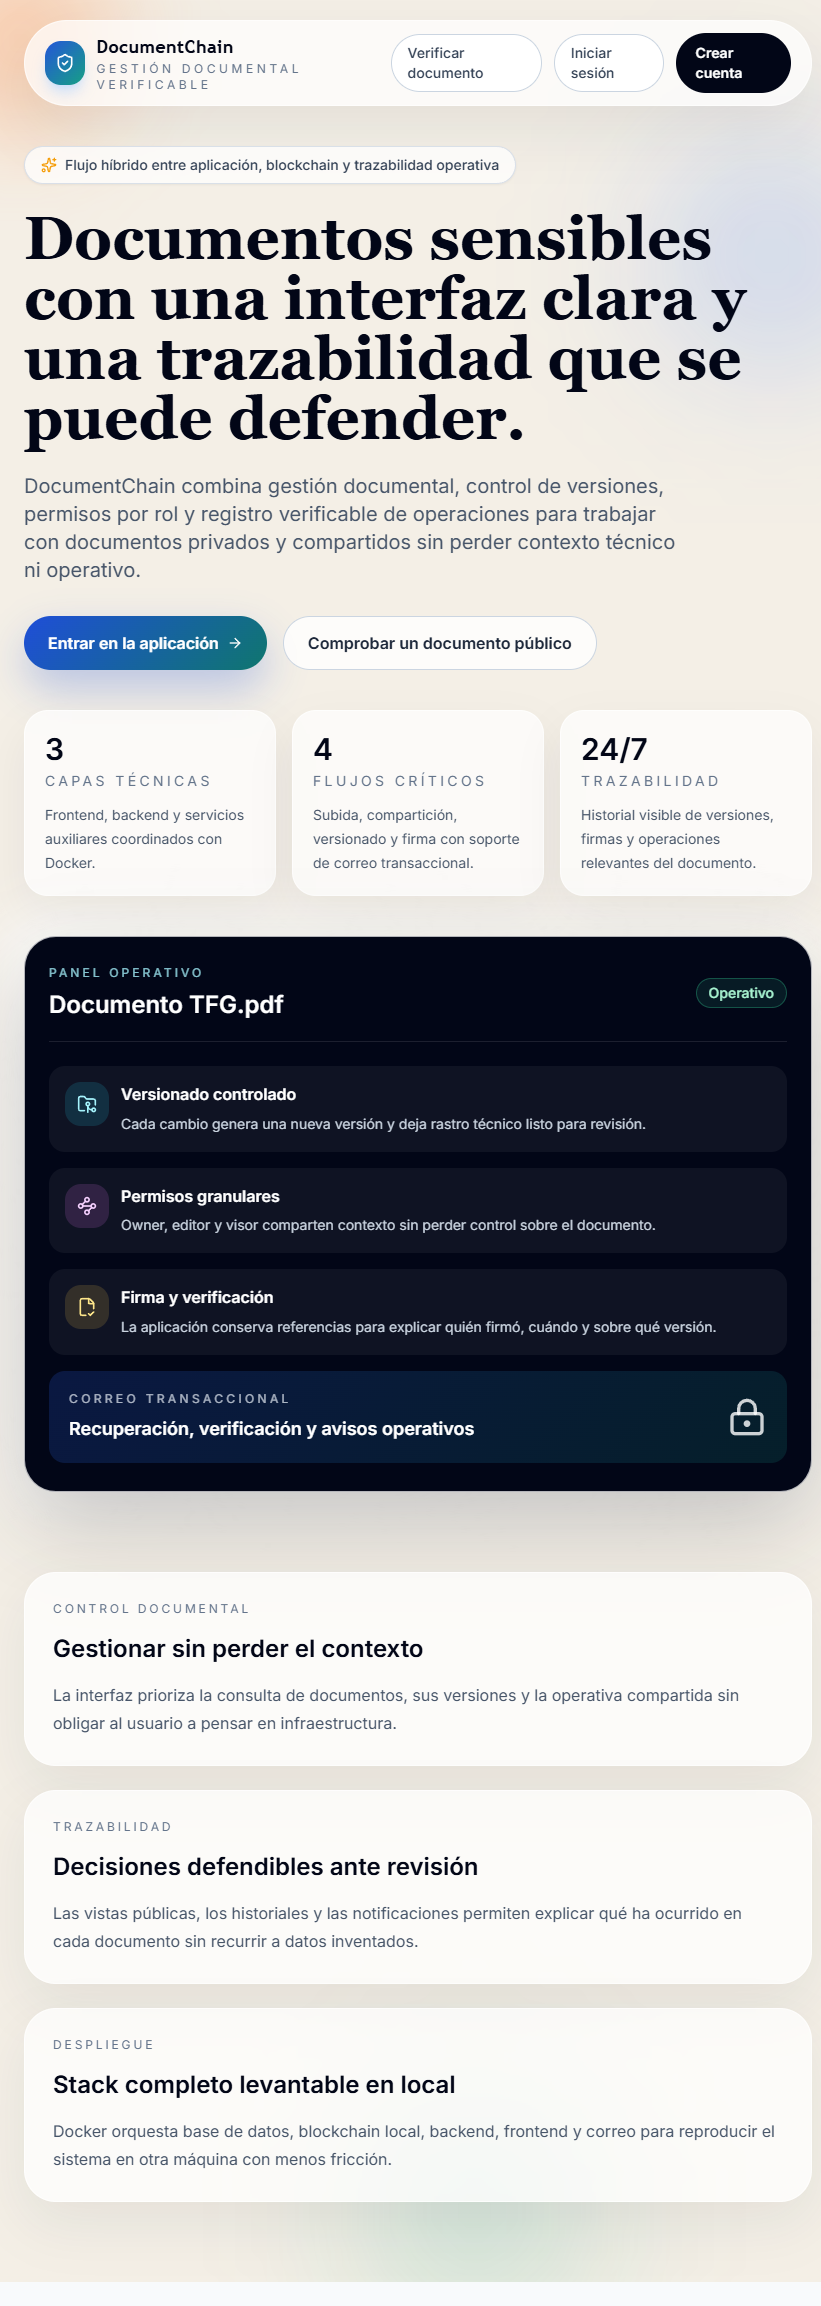
\includegraphics[width=0.95\textwidth]{capturas-ui/landing-public.png}
    \caption{Portada pública de DocumentChain (escritorio)}
    \label{fig:landing-public}
\end{figure}

\begin{figure}[H]
    \centering
    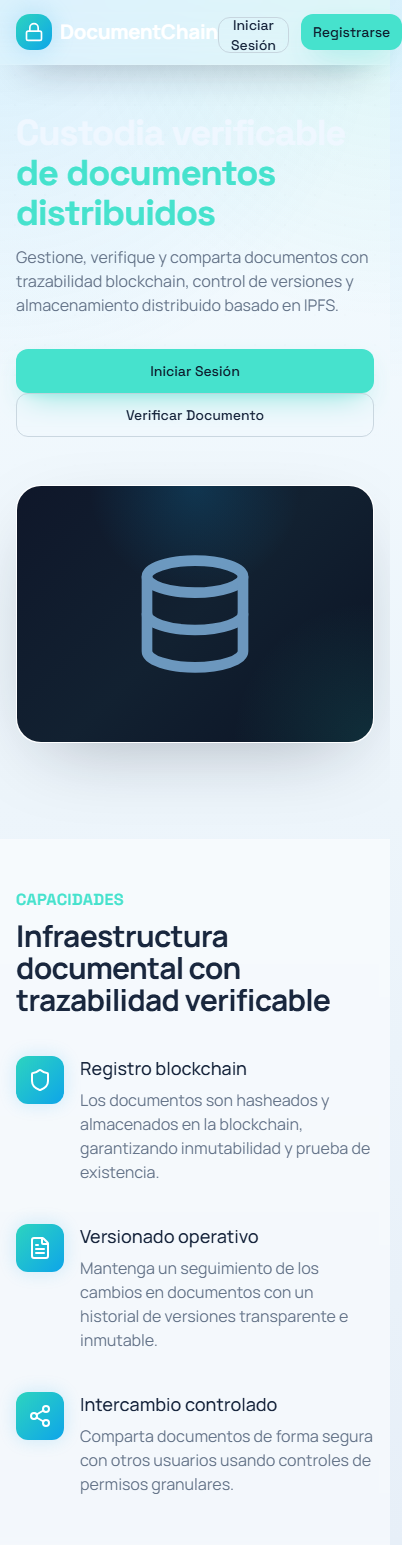
\includegraphics[width=0.45\textwidth]{capturas-ui/mobile-landing.png}
    \caption{Portada pública de DocumentChain (móvil)}
    \label{fig:landing-public-mobile}
\end{figure}

\subsection{Adaptación a dispositivos móviles}

La interfaz de DocumentChain está diseñada con enfoque \textit{responsive}, lo que permite su uso completo desde navegadores móviles. En pantallas pequeñas, la barra lateral de navegación se oculta y se accede a ella mediante el botón de menú hamburguesa situado en la esquina superior derecha. El contenido principal se reestructura en una única columna, los modales ocupan toda la pantalla y las pestañas permiten desplazamiento horizontal cuando es necesario.

\begin{figure}[H]
    \centering
    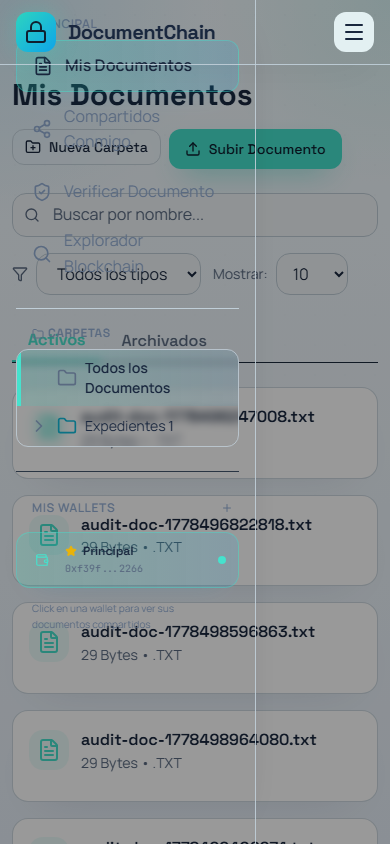
\includegraphics[width=0.45\textwidth]{capturas-ui/mobile-sidebar-open.png}
    \caption{Menú de navegación desplegado en dispositivo móvil}
    \label{fig:mobile-sidebar-open}
\end{figure}

\subsection{Primeros pasos}

\subsubsection{Crear una cuenta}

\begin{enumerate}
    \item Accede a la URL de DocumentChain en tu navegador.
    
    \item En la pantalla de inicio, haz clic en el enlace \textbf{¿No tienes cuenta? Regístrate}.
    
    \begin{figure}[H]
        \centering
        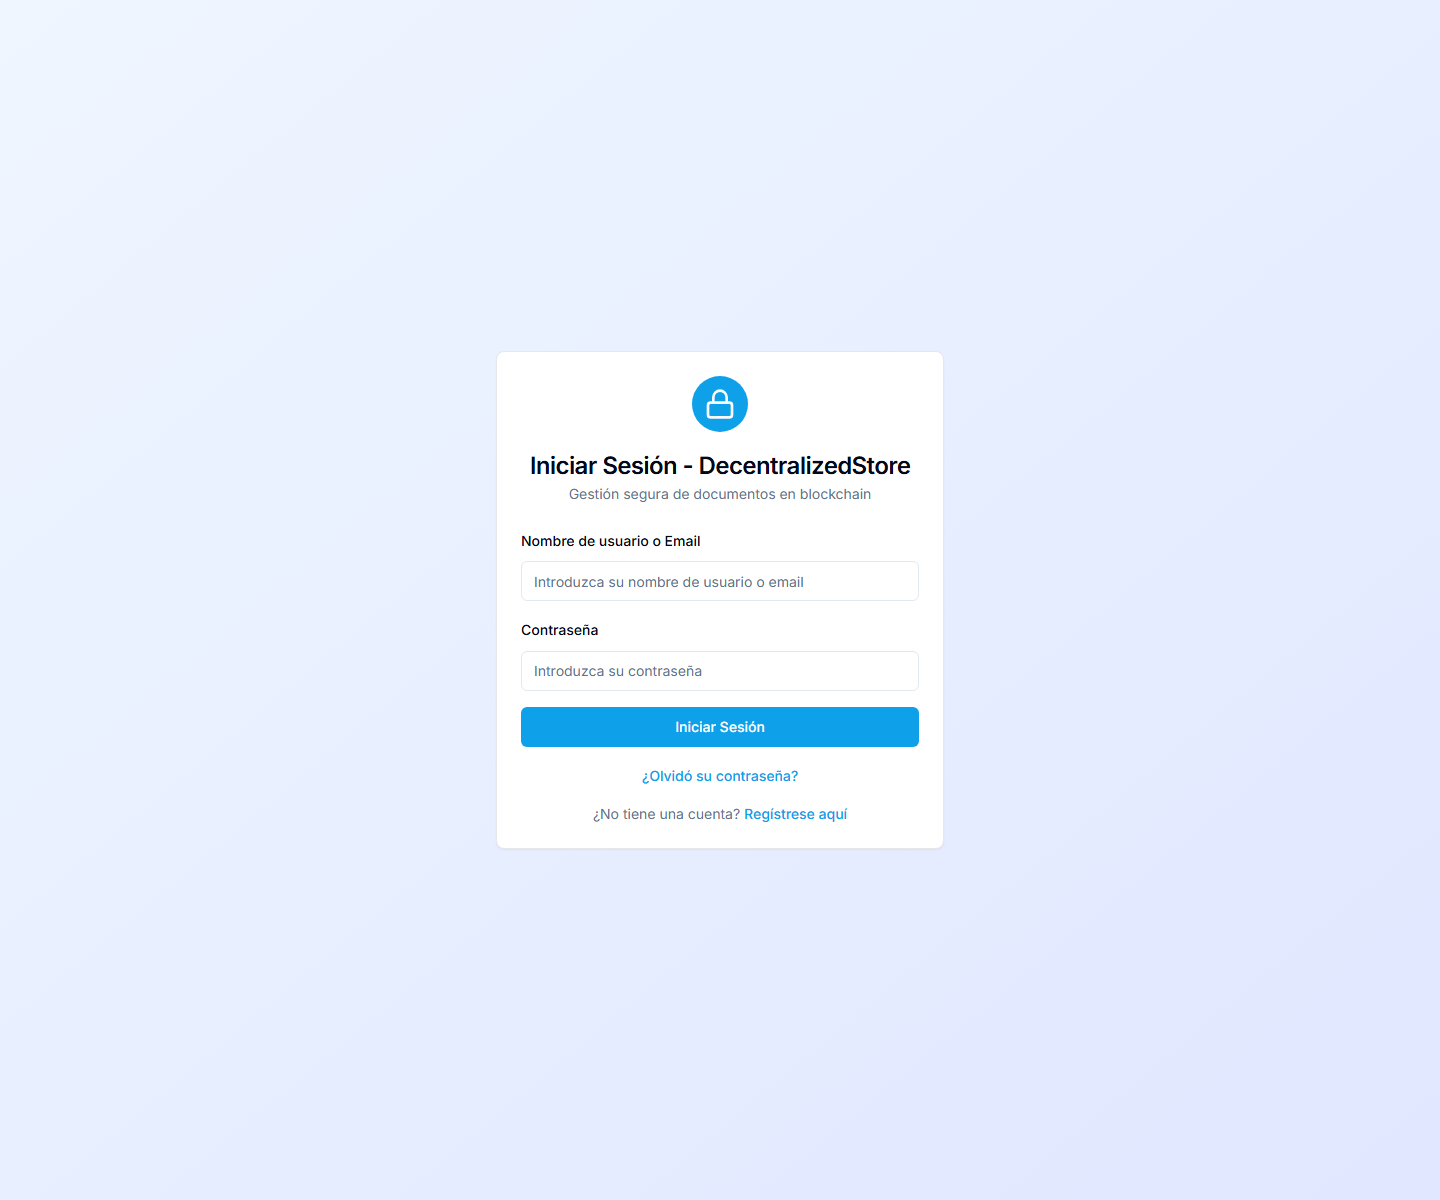
\includegraphics[width=0.95\textwidth]{capturas-ui/login-page.png}
        \caption{Pantalla de inicio de sesión (escritorio)}
        \label{fig:login-page}
    \end{figure}
    
    \begin{figure}[H]
        \centering
        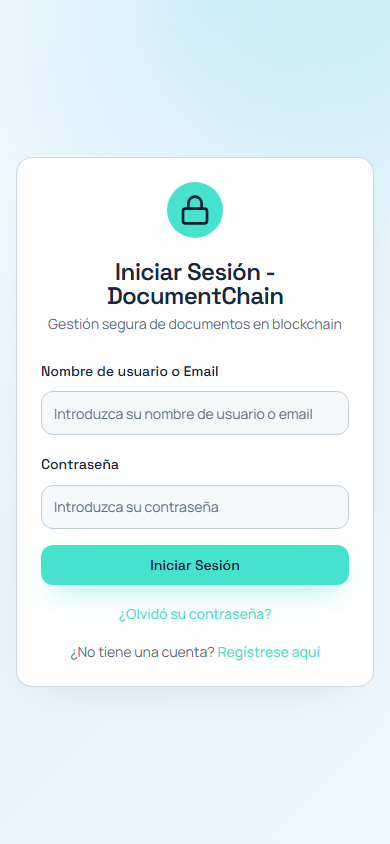
\includegraphics[width=0.45\textwidth]{capturas-ui/mobile-login.png}
        \caption{Pantalla de inicio de sesión (móvil)}
        \label{fig:login-page-mobile}
    \end{figure}
    
    \item Completa el formulario de registro:
    \begin{itemize}
        \item \textbf{Nombre de usuario}: único, entre 3-20 caracteres, solo letras, números y guiones
        \item \textbf{Email}: Dirección de correo válida (recibirás un email de verificación)
        \item \textbf{Contraseña}: Mínimo 8 caracteres con al menos una mayúscula, minúscula, número y símbolo
        \item \textbf{Confirmar contraseña}: Repite la contraseña
        \item \textbf{Nombre completo} (opcional): Tu nombre real para personalización
    \end{itemize}
    
    \begin{figure}[H]
        \centering
        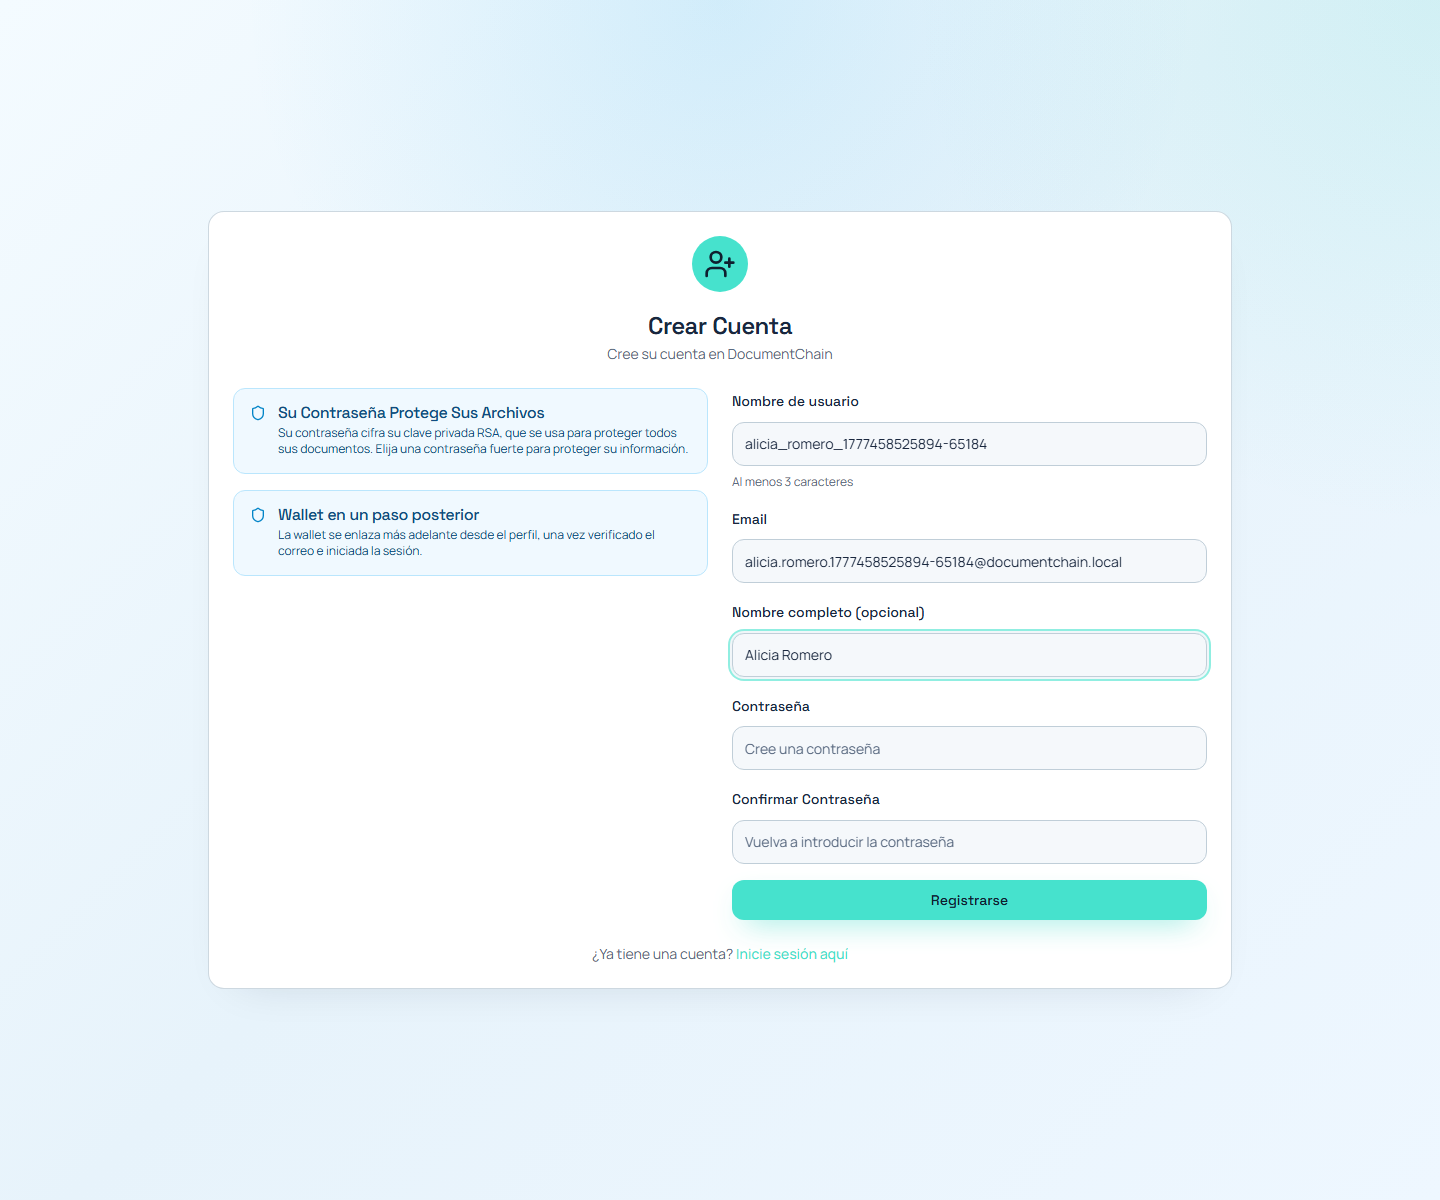
\includegraphics[width=0.95\textwidth]{capturas-ui/register-form.png}
        \caption{Formulario de registro (escritorio)}
        \label{fig:register-form}
    \end{figure}
    
    \begin{figure}[H]
        \centering
        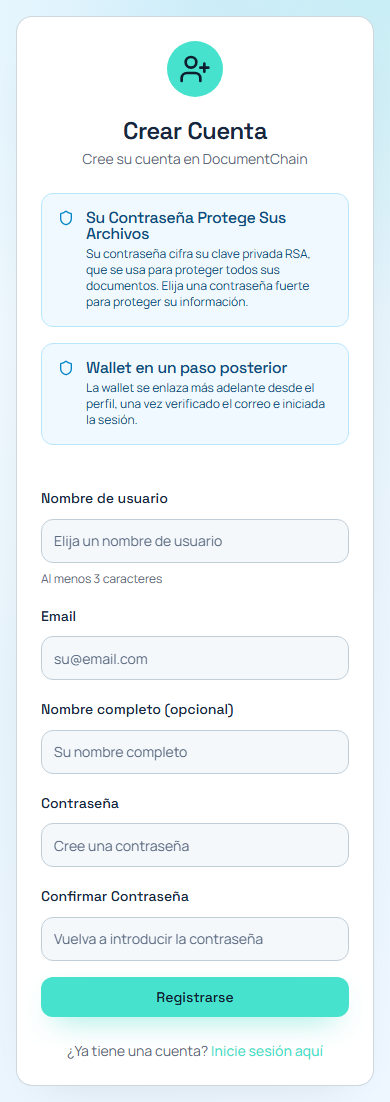
\includegraphics[width=0.45\textwidth]{capturas-ui/mobile-register.png}
        \caption{Formulario de registro (móvil)}
        \label{fig:register-form-mobile}
    \end{figure}
    
    \item \textbf{Importante}: Tras hacer clic en \textbf{Crear Cuenta}, el sistema generará un par de claves criptográficas. Se te mostrará una \textit{Recovery Key} (clave de recuperación). 
    
    \textbf{Guarda esta clave en un lugar seguro}. Es la única forma de recuperar tu cuenta si olvidas la contraseña.
    
    \begin{figure}[H]
        \centering
        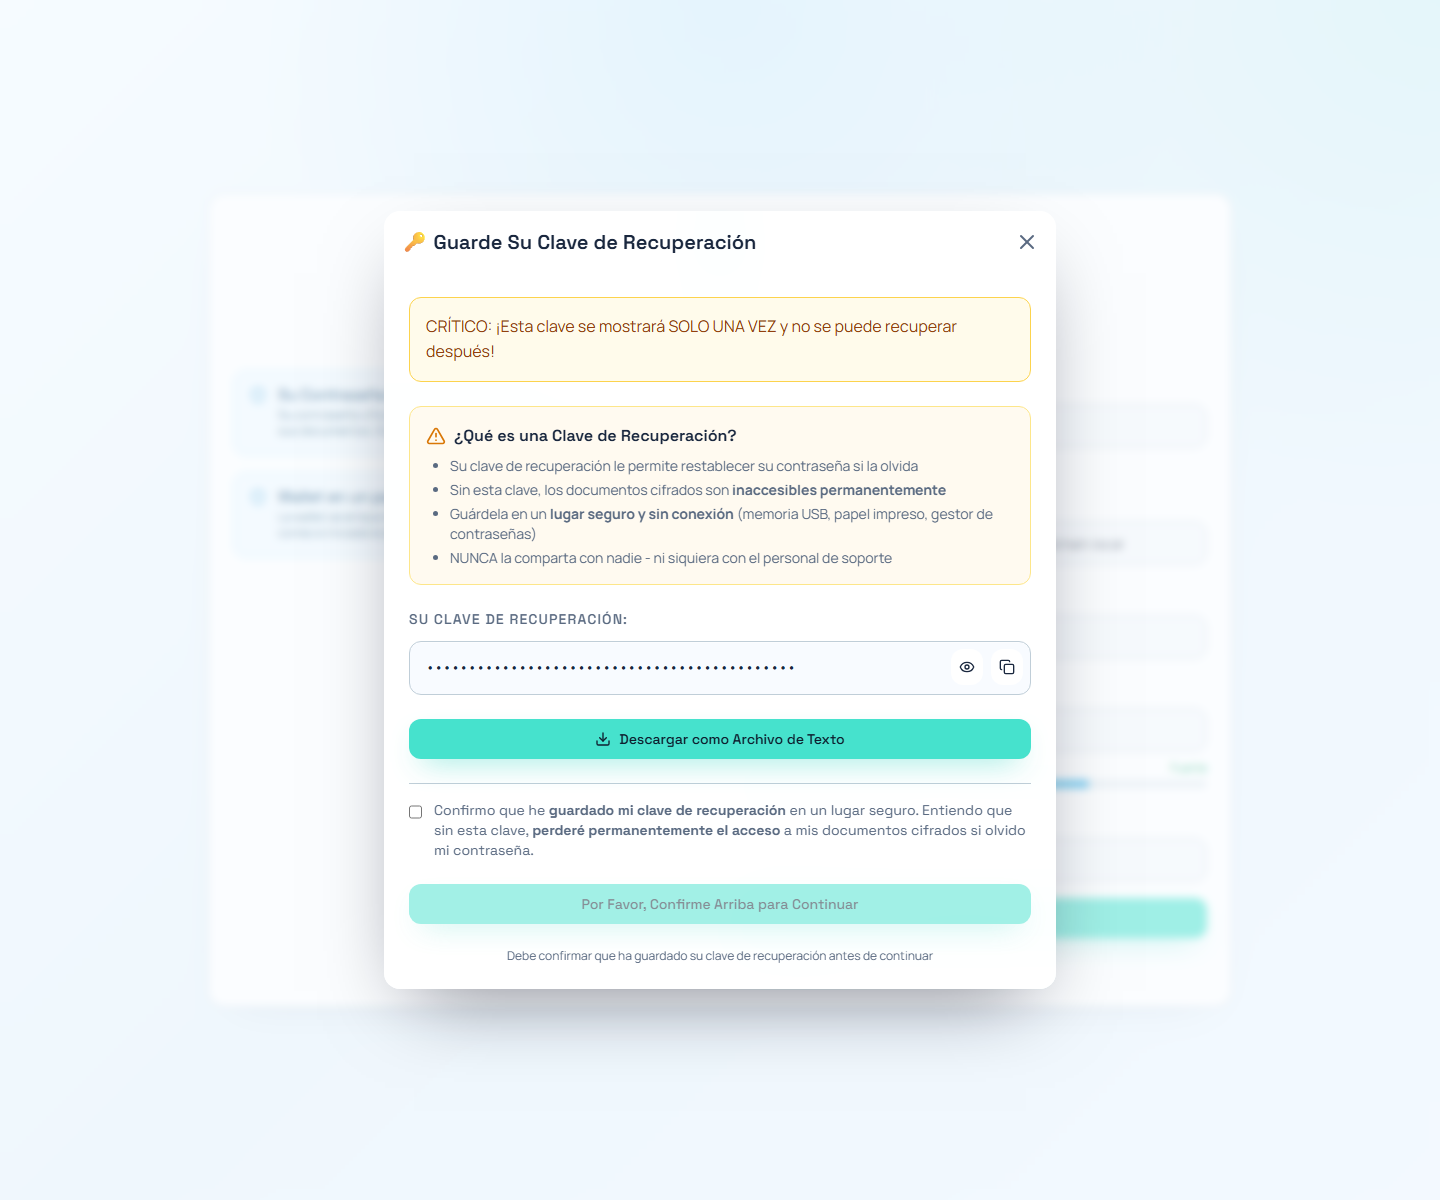
\includegraphics[width=0.8\textwidth]{capturas-ui/recovery-key-modal.png}
        \caption{Modal con Recovery Key}
        \label{fig:recovery-key}
    \end{figure}
    
    \item Descarga la Recovery Key haciendo clic en \textbf{Descargar clave} o cópiala manualmente.
    
    \item Marca la casilla \textbf{He guardado mi clave de recuperación de forma segura} y haz clic en \textbf{Continuar}.
    
    \item El sistema mostrará una pantalla de confirmación indicando que la cuenta ya ha sido creada, pero que todavía no es posible acceder al área privada hasta verificar el correo.
    
    \item Recibirás un email de verificación. Abre tu bandeja de entrada y haz clic en el enlace de verificación.
    
    \item Tras esa confirmación ya podrás iniciar sesión con normalidad.
\end{enumerate}

\textbf{Nota}: En la versión actual, los documentos privados se protegen criptográficamente y solo pueden descargarse con las credenciales adecuadas. Los documentos públicos siguen otro flujo: se publican sin cifrar porque están destinados a ser accesibles mediante enlace compartible.

\subsubsection{Confirmar el correo electrónico}

Tras completar el registro, o cuando cambias el email desde la configuración de la cuenta, el sistema envía un enlace específico a la ruta \texttt{/verify-email}.

\begin{enumerate}
    \item Abre el mensaje recibido en tu correo electrónico.
    \item Pulsa el enlace de verificación incluido en el mensaje.
    \item La pantalla mostrará uno de estos resultados:
    \begin{itemize}
        \item \textbf{Verificación correcta}: la cuenta queda confirmada y ya puede iniciarse sesión con normalidad.
        \item \textbf{Verificación pendiente}: si la cuenta ya tiene sesión pero sigue bloqueada, la pantalla avisará de que falta confirmar el correo y ofrecerá un reenvío.
        \item \textbf{Error de verificación}: el token no es válido, ha caducado o falta en la URL. En ese caso también puede solicitarse un nuevo mensaje desde la propia pantalla.
    \end{itemize}
    \item Desde esa misma página puedes volver a \textbf{Iniciar sesión}, regresar al formulario de \textbf{Registro} o reenviar la verificación si todavía no ha llegado el mensaje válido.
\end{enumerate}

El mensaje recibido incluye un único botón principal con acceso directo al flujo de verificación. Se ha mantenido un diseño sencillo para favorecer la legibilidad en proveedores de correo habituales y para reducir el riesgo de que el mensaje sea interpretado como contenido promocional.

\begin{figure}[H]
    \centering
    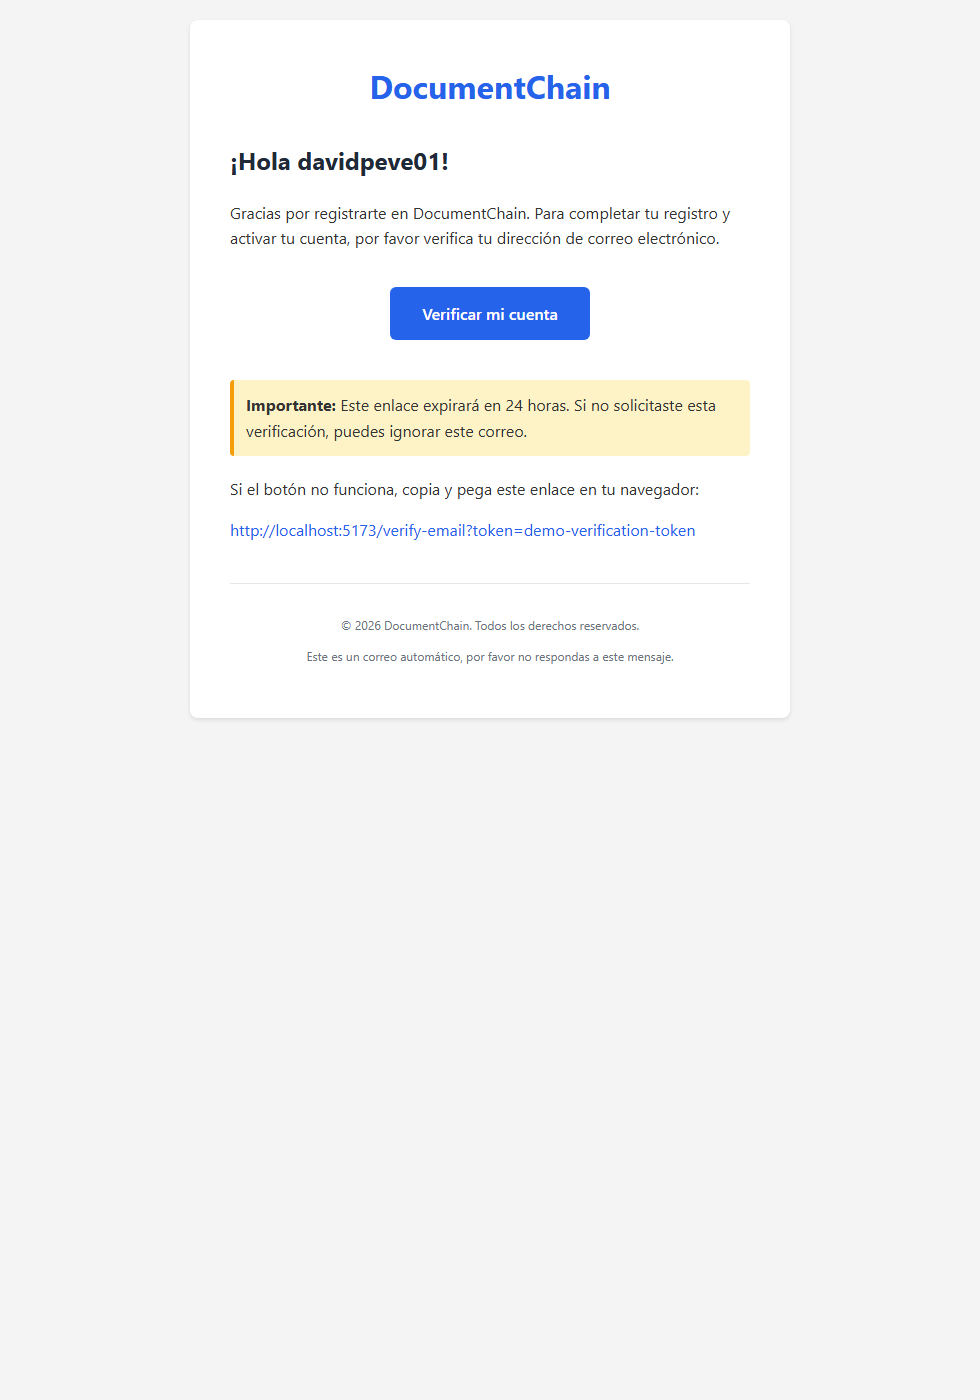
\includegraphics[width=0.78\textwidth]{capturas-ui/email-verification-preview.png}
    \caption{Correo de verificación de cuenta}
    \label{fig:email-verification-preview}
\end{figure}

\subsubsection{Iniciar sesión}

El acceso al sistema se realiza con \textbf{nombre de usuario o email} y \textbf{contraseña}. Si la cuenta tiene activada la autenticación de dos factores, tras validar las credenciales se solicitará un \textbf{código 2FA} o uno de los \textbf{códigos de respaldo}.

\begin{enumerate}
    \item En la pantalla de inicio, introduce tu \textbf{nombre de usuario o email}.
    \item Introduce tu \textbf{contraseña}.
    \item Haz clic en \textbf{Iniciar Sesión}.
    \item Si el correo de la cuenta todavía no está verificado, el sistema bloqueará el acceso y mostrará un enlace para reenviar la verificación.
    \item Si la cuenta tiene 2FA activo y el correo ya está verificado, se abrirá una segunda pantalla de verificación.
    \item Introduce el código temporal de tu aplicación autenticadora o uno de los códigos de respaldo válidos.
    \item Tras completar la validación, accederás a la vista principal de documentos.
\end{enumerate}

\begin{figure}[H]
    \centering
    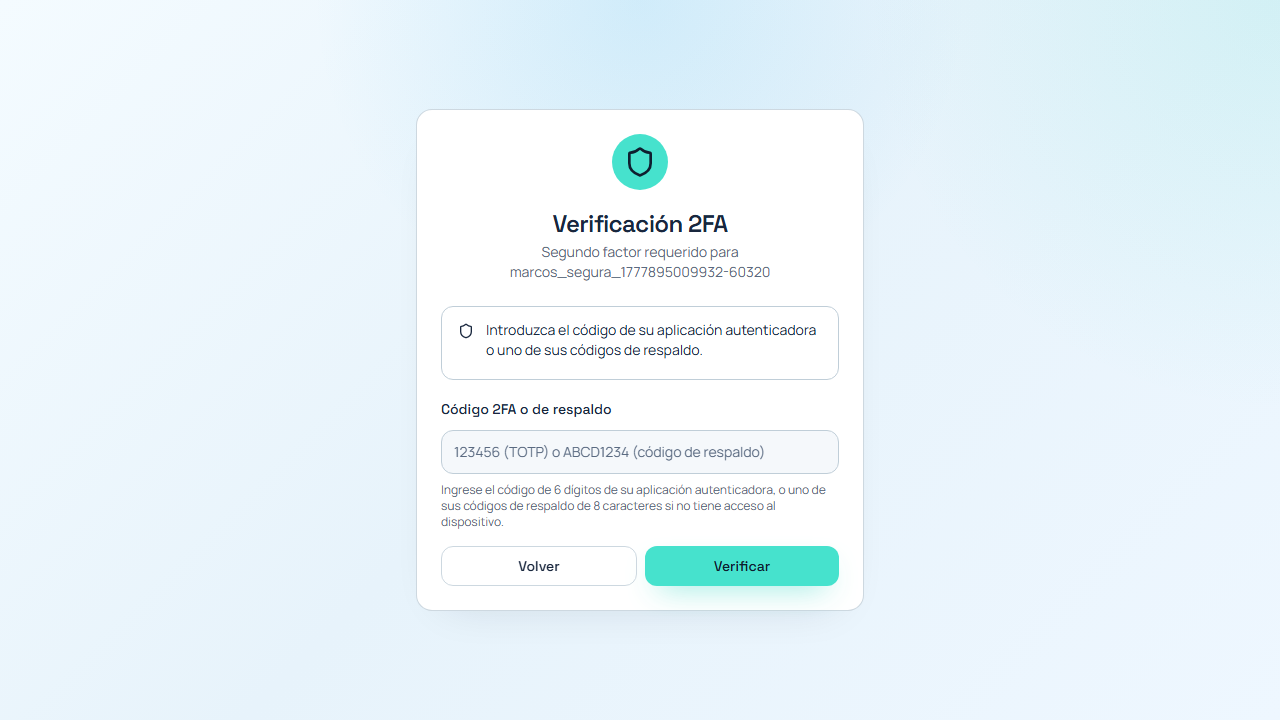
\includegraphics[width=0.72\textwidth]{capturas-ui/two-factor-login.png}
    \caption{Pantalla de verificación de segundo factor durante el inicio de sesión}
    \label{fig:two-factor-login}
\end{figure}

\textbf{Nota}: En la interfaz entregada, las wallets \textbf{no} se utilizan para iniciar sesión ni para completar el registro habitual. Su uso visible para el usuario queda reservado a la firma de operaciones blockchain, como subida, compartición, firmado o reactivación de cuenta.

\subsubsection{Cerrar sesión}

El cierre de sesión está disponible desde la cabecera superior, tanto en escritorio como en la versión móvil.

\begin{enumerate}
    \item Pulsa el icono \textbf{Cerrar sesión} de la cabecera.
    \item El cliente invalidará la sesión local y notificará el cierre al backend.
    \item Tras completarse la operación, volverás a la pantalla pública de acceso.
\end{enumerate}

\subsubsection{Recuperar contraseña}

Si olvidaste tu contraseña:

\begin{enumerate}
    \item En la pantalla de inicio, haz clic en \textbf{¿Olvidaste tu contraseña?}.
    \item Introduce tu \textbf{email} registrado.
    \item Recibirás un email con un enlace de recuperación (válido por 1 hora).
    \item Haz clic en el enlace y se abrirá una página para crear nueva contraseña.
    \item Introduce tu \textbf{Recovery Key} (la que guardaste al registrarte).
    \item Crea una nueva contraseña y confírmala.
    \item Haz clic en \textbf{Restablecer Contraseña}.
\end{enumerate}

\textbf{Advertencia}: Si no tienes la Recovery Key, no podrás recuperar tu cuenta ni tus documentos cifrados. Es \textbf{imposible} descifrarlos sin la clave privada.

Cuando se solicita el restablecimiento, el sistema envía un correo transaccional con un enlace temporal y un recordatorio del tiempo de expiración. El acceso conducirá a la pantalla \texttt{/reset-password}, donde se pedirá la nueva contraseña y la Recovery Key asociada a la cuenta.

\begin{figure}[H]
    \centering
    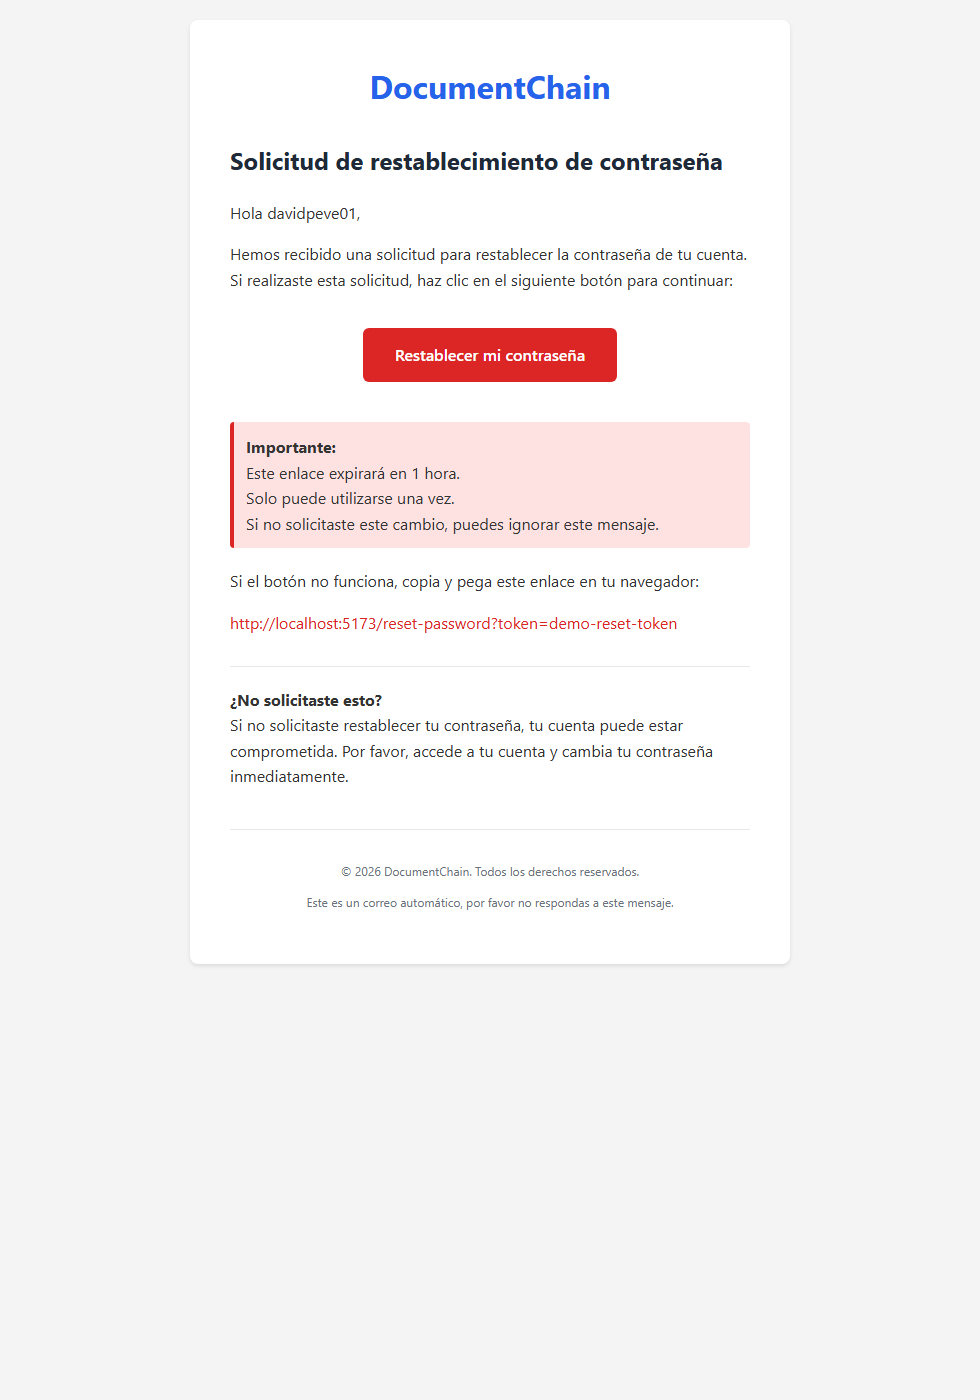
\includegraphics[width=0.78\textwidth]{capturas-ui/email-password-reset-preview.png}
    \caption{Correo de restablecimiento de contraseña}
    \label{fig:email-password-reset-preview}
\end{figure}

\subsection{Vista principal de documentos}

Tras iniciar sesión, el sistema redirige a \texttt{/app/documents}, que actúa como punto de entrada principal.

\begin{figure}[H]
    \centering
    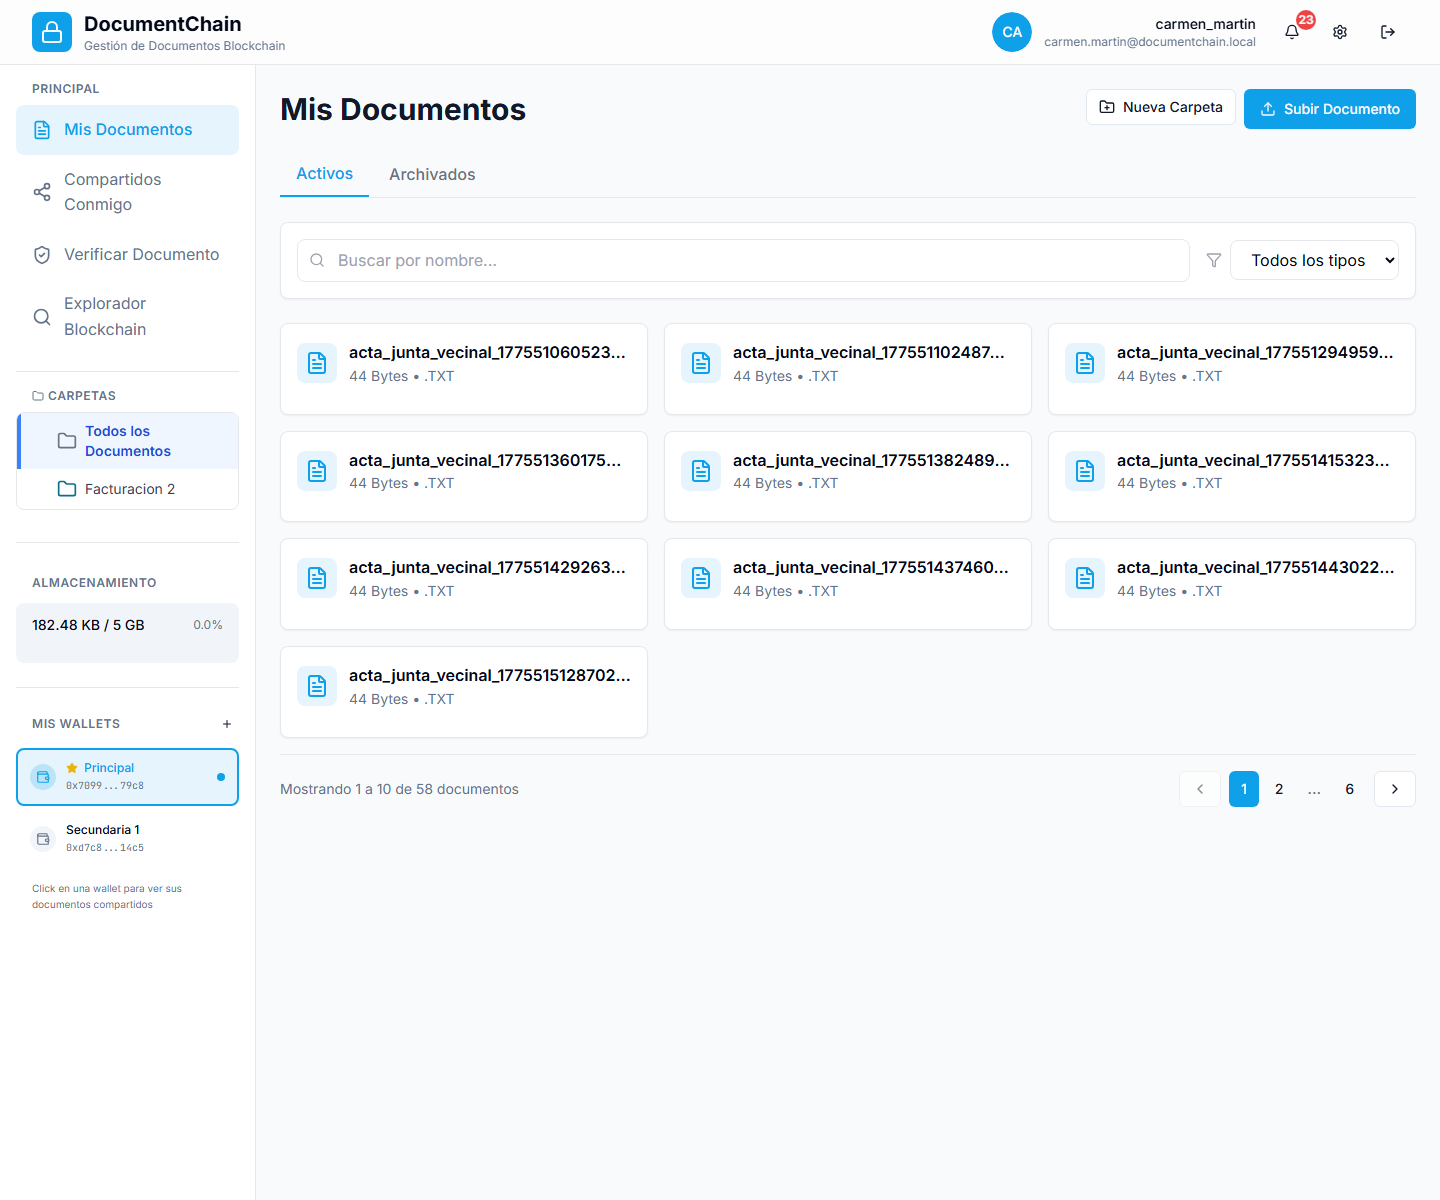
\includegraphics[width=0.95\textwidth]{capturas-ui/documents-page.png}
    \caption{Panel principal con listado de documentos (escritorio)}
    \label{fig:documents-page}
\end{figure}

\begin{figure}[H]
    \centering
    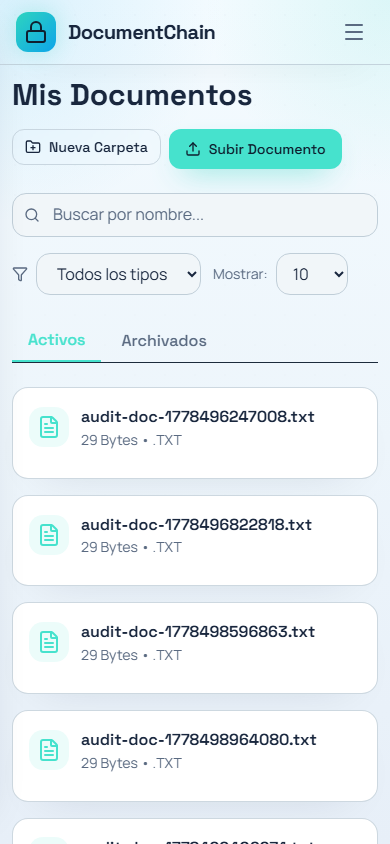
\includegraphics[width=0.45\textwidth]{capturas-ui/mobile-documents-list.png}
    \caption{Panel principal con listado de documentos (móvil)}
    \label{fig:documents-page-mobile}
\end{figure}

\subsubsection{Elementos principales}

\begin{enumerate}
    \item \textbf{Cabecera superior}:
    \begin{itemize}
        \item Identidad visual de DocumentChain
        \item Información resumida de la sesión del usuario
        \item Accesos directos a \textbf{Notificaciones}, \textbf{Configuración} y \textbf{Cerrar sesión}
    \end{itemize}
    
    \item \textbf{Sidebar izquierdo}:
    \begin{itemize}
        \item \textbf{Mis Documentos}: colección propia del usuario
        \item \textbf{Compartidos Conmigo}: documentos accesibles con la wallet activa
        \item \textbf{Verificar Documento}: herramienta de comprobación manual
        \item \textbf{Explorador Blockchain}: visor técnico de eventos y transacciones
        \item Árbol de \textbf{carpetas} cuando se está en la vista de documentos
        \item Widget de \textbf{almacenamiento} utilizado
        \item Selector de \textbf{wallets guardadas}
    \end{itemize}
    
    \item \textbf{Área principal}:
    \begin{itemize}
        \item Botones \textbf{Nueva Carpeta} y \textbf{Subir Documento}
        \item Pestañas \textbf{Activos} y \textbf{Archivados}
        \item Búsqueda por nombre y filtro por tipo de archivo
        \item Listado paginado de documentos con acceso directo al detalle
    \end{itemize}
\end{enumerate}

\subsection{Gestión de documentos}

\subsubsection{Subir un documento}

\begin{enumerate}
    \item Haz clic en el botón \textbf{+ Subir Documento} en el Dashboard.
    
    \item Se abrirá un modal con un formulario. Puedes subir el archivo de dos formas:
    \begin{itemize}
        \item \textbf{Drag \& drop}: Arrastra el archivo a la zona indicada
        \item \textbf{Click}: Haz clic en "Seleccionar archivo" y busca el archivo en tu ordenador
    \end{itemize}
    
    \begin{figure}[H]
        \centering
        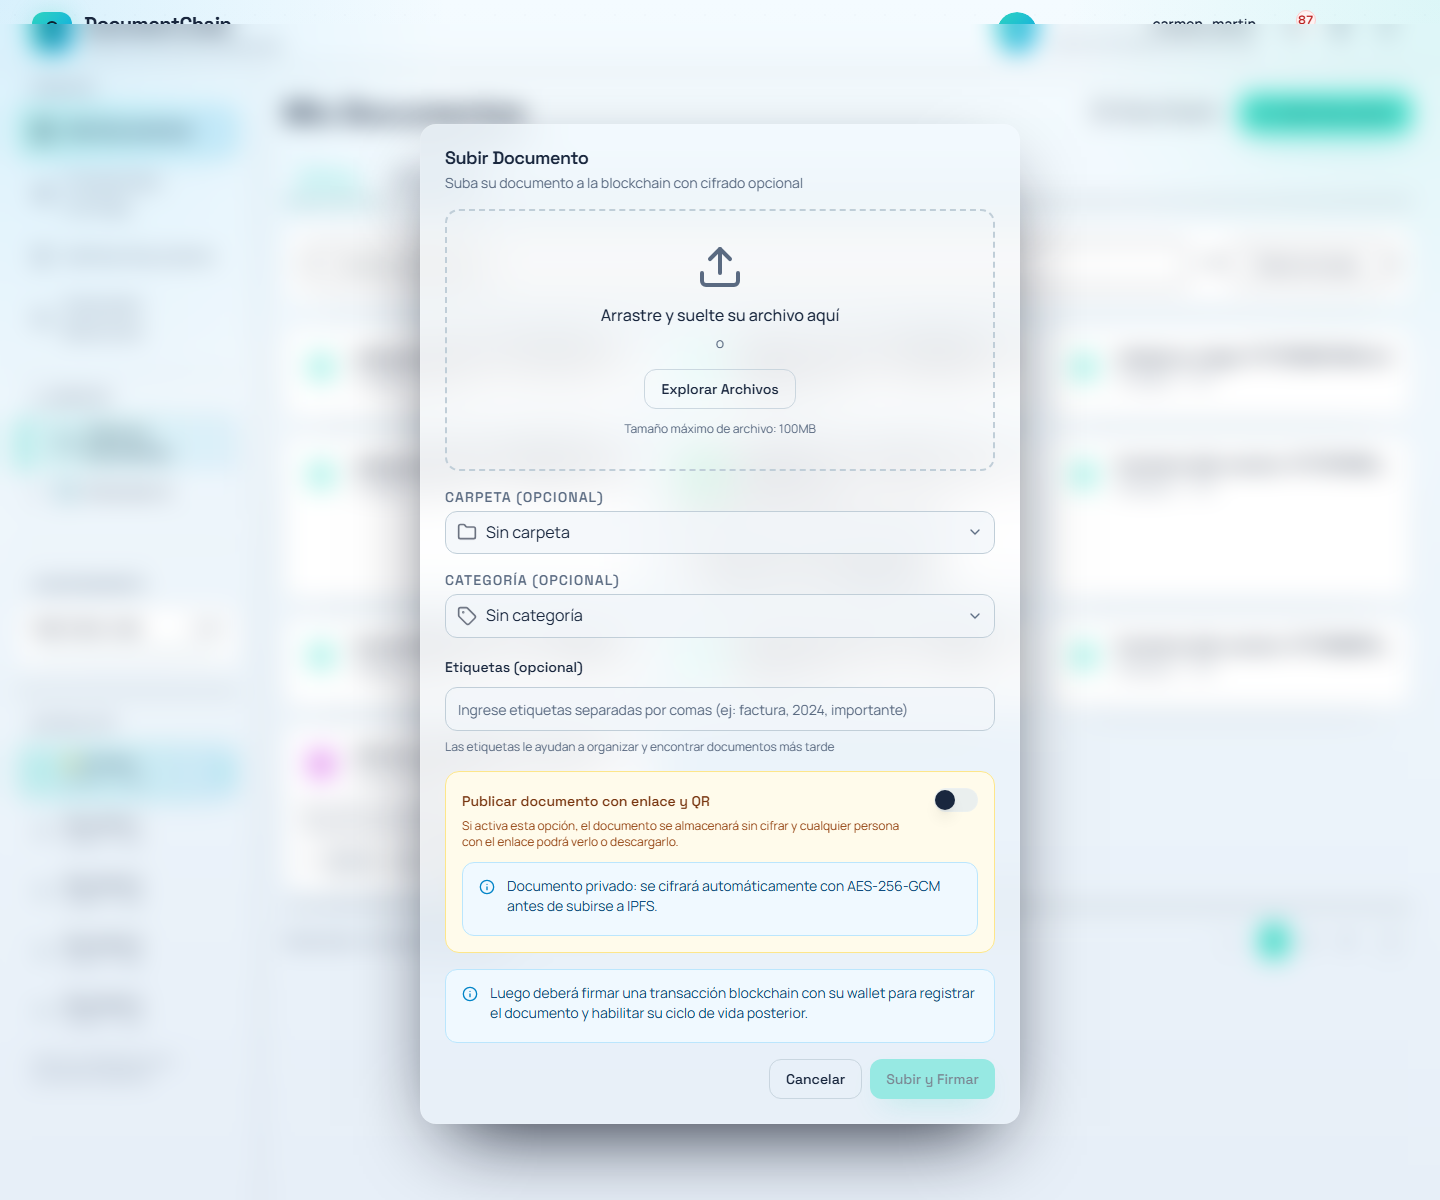
\includegraphics[width=0.85\textwidth]{capturas-ui/upload-modal.png}
        \caption{Modal de subida de documento (escritorio)}
        \label{fig:upload-modal}
    \end{figure}
    
    \begin{figure}[H]
        \centering
        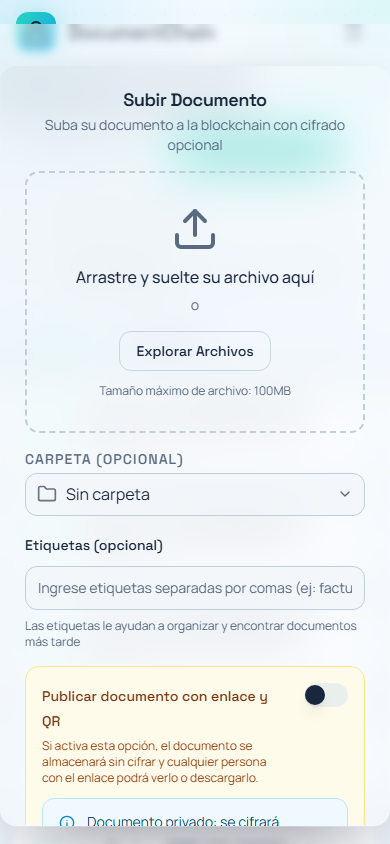
\includegraphics[width=0.45\textwidth]{capturas-ui/mobile-upload-modal.png}
        \caption{Modal de subida de documento (móvil)}
        \label{fig:upload-modal-mobile}
    \end{figure}
    
    \item Completa la información disponible en el formulario:
    \begin{itemize}
        \item \textbf{Archivo}: documento a registrar
        \item \textbf{Carpeta} (opcional): Ubica el documento en una carpeta
        \item \textbf{Etiquetas} (opcional): añade términos separados por comas
        \item \textbf{Visibilidad}: decide si el documento será privado o público
    \end{itemize}
    
    \item Si activas \textbf{Publicar documento con enlace y QR}, la propia interfaz mostrará una advertencia: ese archivo se almacenará sin cifrar y cualquier persona con el enlace podrá verlo o descargarlo.

    \item Si dejas la opción desactivada, el documento seguirá el flujo privado habitual.

    \item El sistema preparará el documento según la visibilidad elegida y solicitará una wallet para firmar la operación blockchain.

    \begin{figure}[H]
        \centering
        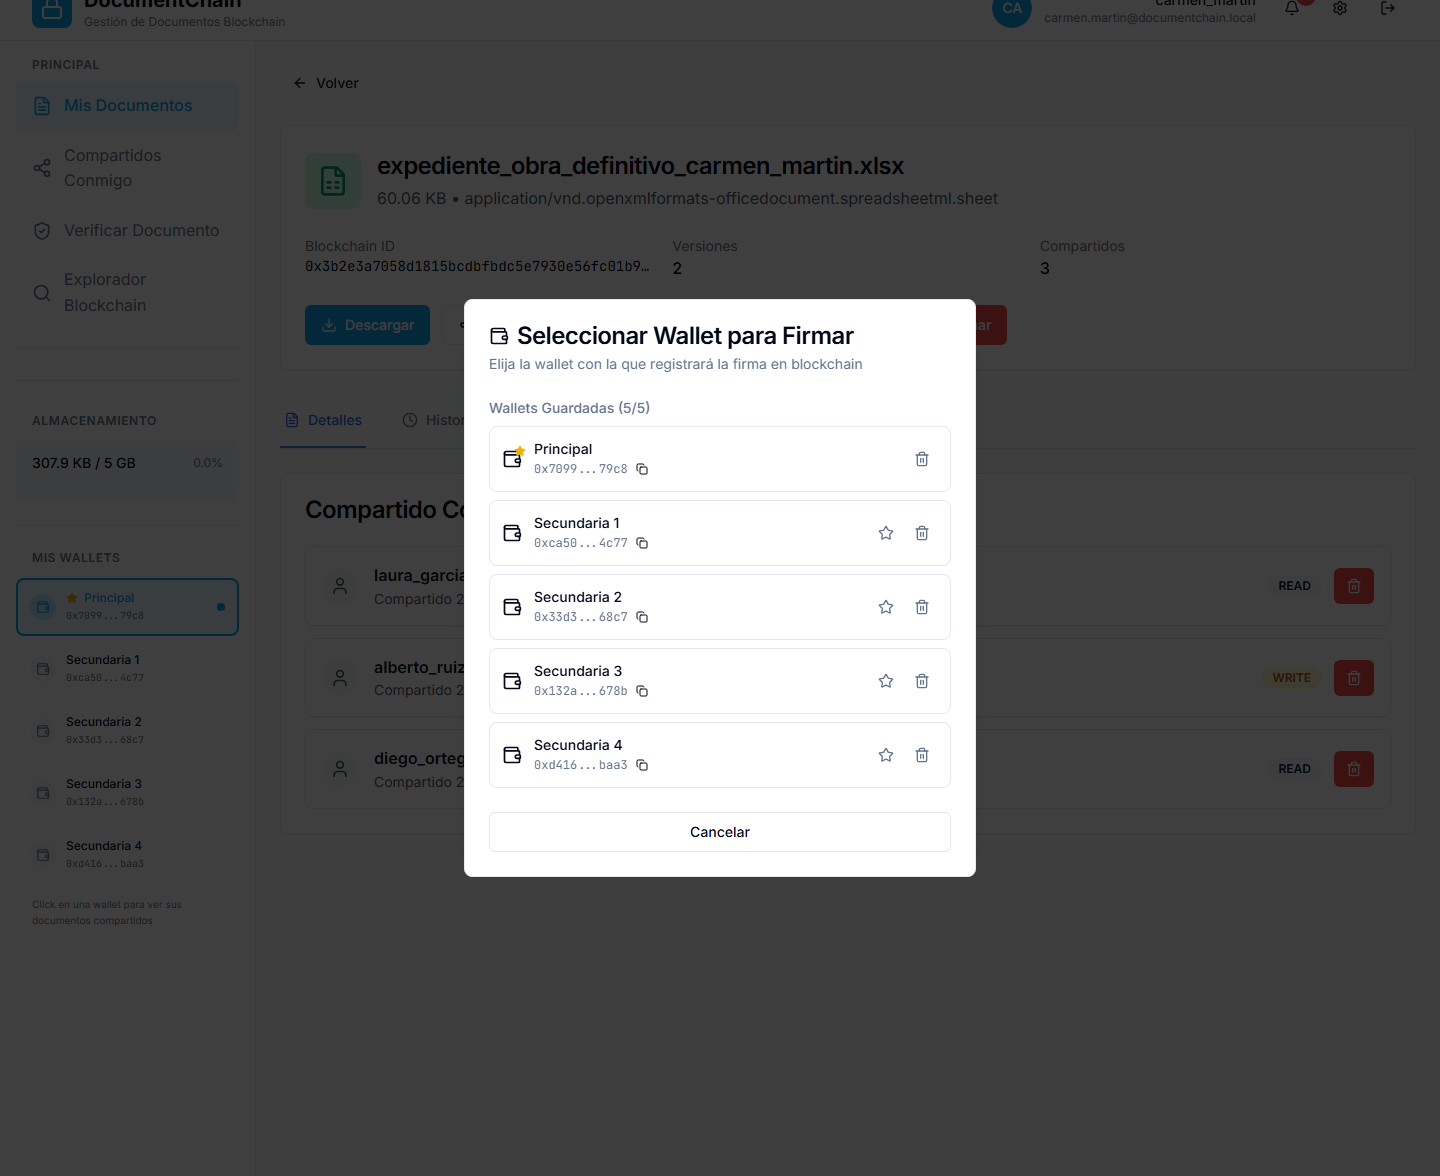
\includegraphics[width=0.72\textwidth]{capturas-ui/wallet-selector-modal.png}
        \caption{Selector de wallet para firmar la transacción blockchain (escritorio)}
        \label{fig:wallet-selector}
    \end{figure}
    
    \begin{figure}[H]
        \centering
        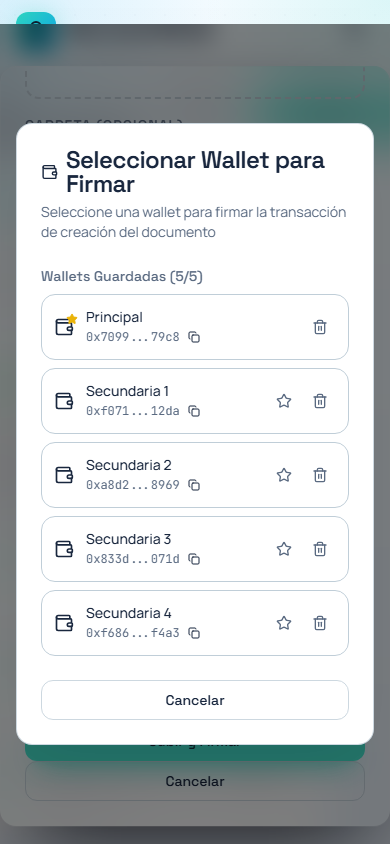
\includegraphics[width=0.45\textwidth]{capturas-ui/mobile-wallet-selector.png}
        \caption{Selector de wallet para firmar la transacción blockchain (móvil)}
        \label{fig:wallet-selector-mobile}
    \end{figure}
    
    \item Haz clic en \textbf{Subir y Firmar}.
    
    \item El sistema mostrará el progreso de preparación, firma y confirmación en blockchain.
    
    \item Confirma la transacción en la wallet conectada y espera a que el registro cambie a estado sincronizado.
    
    \item Cuando finalice el proceso, el documento aparecerá en la lista principal y podrá abrirse desde el detalle. Si es público, en esa vista se habilitarán el enlace y el código QR.
\end{enumerate}

\textbf{Consejo}: Si la firma o la confirmación fallan, el propio asistente de subida mostrará el estado alcanzado para que puedas repetir la operación.

\textbf{Advertencia}: Un documento público deja de comportarse como un documento privado compartido. No requiere contraseña para su descarga y puede circular fuera de la plataforma mientras el contenido siga disponible en IPFS o en gateways que lo hayan replicado.

\textbf{Límites}: La interfaz actual muestra un límite de 100 MB por archivo.

\subsubsection{Buscar documentos}

\begin{enumerate}
    \item En la barra de búsqueda del Navbar, escribe palabras clave.
    \item La búsqueda encuentra coincidencias en el nombre del documento. Para acotar por carpeta, utiliza el árbol lateral; para filtrar por etiquetas o tipo de archivo, expande los filtros avanzados.
    \item Presiona Enter o haz clic en el icono de lupa.
    \item Los resultados se mostrarán en el Área principal.
\end{enumerate}

\textbf{Filtros avanzados}:

\begin{itemize}
    \item \textbf{Por tipo de archivo}: selecciona extensiones frecuentes como PDF, DOCX, TXT, JPG o PNG
    \item \textbf{Por estado visual}: alterna entre \textbf{Activos} y \textbf{Archivados}
    \item \textbf{Por carpeta}: usa el árbol lateral para acotar la vista a una carpeta concreta
\end{itemize}

\subsubsection{Ver detalles de un documento}

\begin{enumerate}
    \item En la lista de documentos, haz clic en el nombre del documento o en el botón \textbf{Ver detalles}.
    
    \begin{figure}[H]
        \centering
        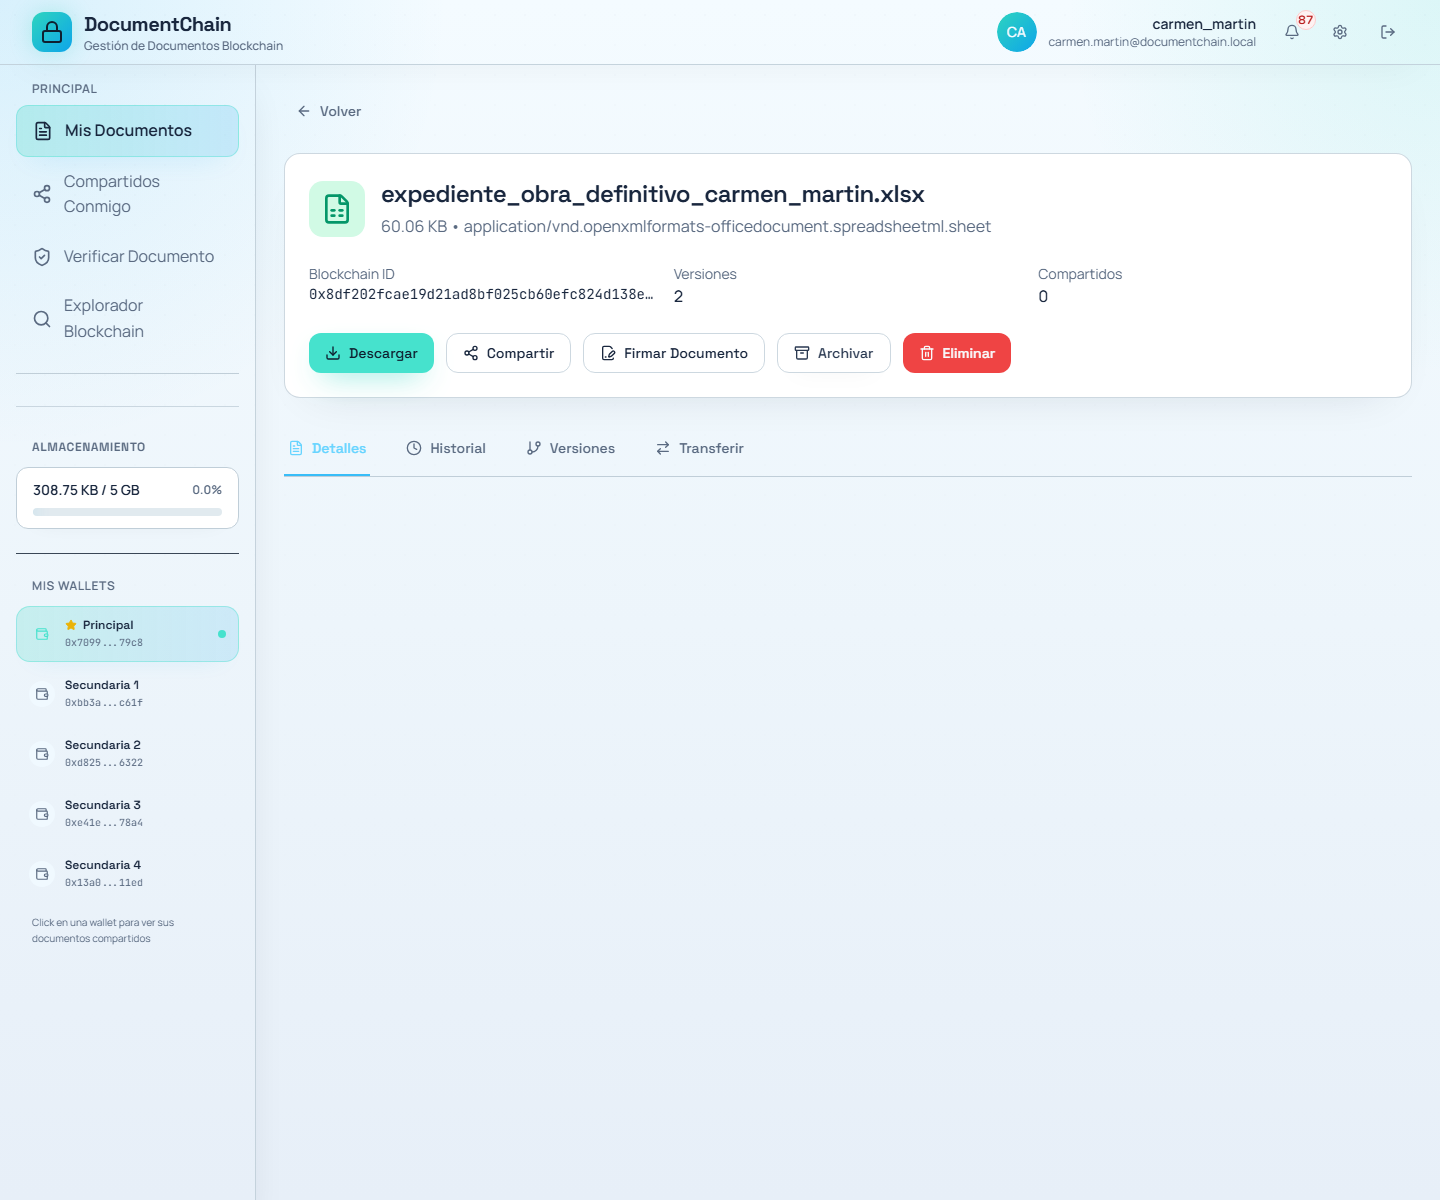
\includegraphics[width=0.95\textwidth]{capturas-ui/document-detail.png}
        \caption{Vista de detalle de un documento (escritorio)}
        \label{fig:document-detail}
    \end{figure}
    
    \begin{figure}[H]
        \centering
        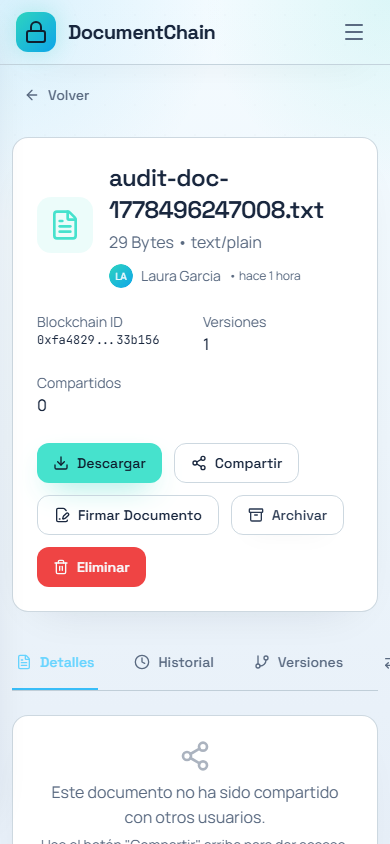
\includegraphics[width=0.45\textwidth]{capturas-ui/mobile-document-detail.png}
        \caption{Vista de detalle de un documento (móvil)}
        \label{fig:document-detail-mobile}
    \end{figure}
    
    \item Verás la información completa:
    \begin{itemize}
        \item Nombre, tamaño y tipo MIME del documento
        \item Identificador interno del documento (\texttt{documentId}) con botón para copiar al portapapeles
        \item Identificador blockchain del registro (\texttt{blockchainId}) con botón para copiar al portapapeles
        \item Número de versiones existentes
        \item Número de accesos compartidos vigentes
        \item Acciones disponibles según el rol del usuario, la visibilidad y el estado del documento
    \end{itemize}
    
    \item Ambos identificadores muestran un tooltip explicativo al pasar el cursor: el \texttt{documentId} es el identificador interno de la base de datos, mientras que el \texttt{blockchainId} es el identificador asignado por el contrato Ethereum. El botón de copia permite trasladar el valor completo al portapapeles con un solo clic.
    
    \item Pestañas disponibles:
    \begin{itemize}
        \item \textbf{Detalles}: muestra los accesos compartidos cuando existen y, en documentos públicos, las acciones de enlace y QR
        \item \textbf{Historial}: resume eventos del documento
        \item \textbf{Versiones}: historial de versiones y activación de versión operativa
        \item \textbf{Transferir}: disponible únicamente para el propietario
    \end{itemize}
    
    \item \textbf{Nota}: El bloque superior del detalle muestra el avatar y el nombre del propietario cuando éste ha configurado una imagen de perfil.
\end{enumerate}

\subsubsection{Descargar un documento}

\begin{enumerate}
    \item Desde la vista de detalles, haz clic en el botón \textbf{Descargar} (icono de descarga).
    
    \item Si el documento es privado, se abrirá un modal solicitando tu contraseña. Esto es necesario para descifrar tu clave privada.
    
    \begin{figure}[H]
        \centering
        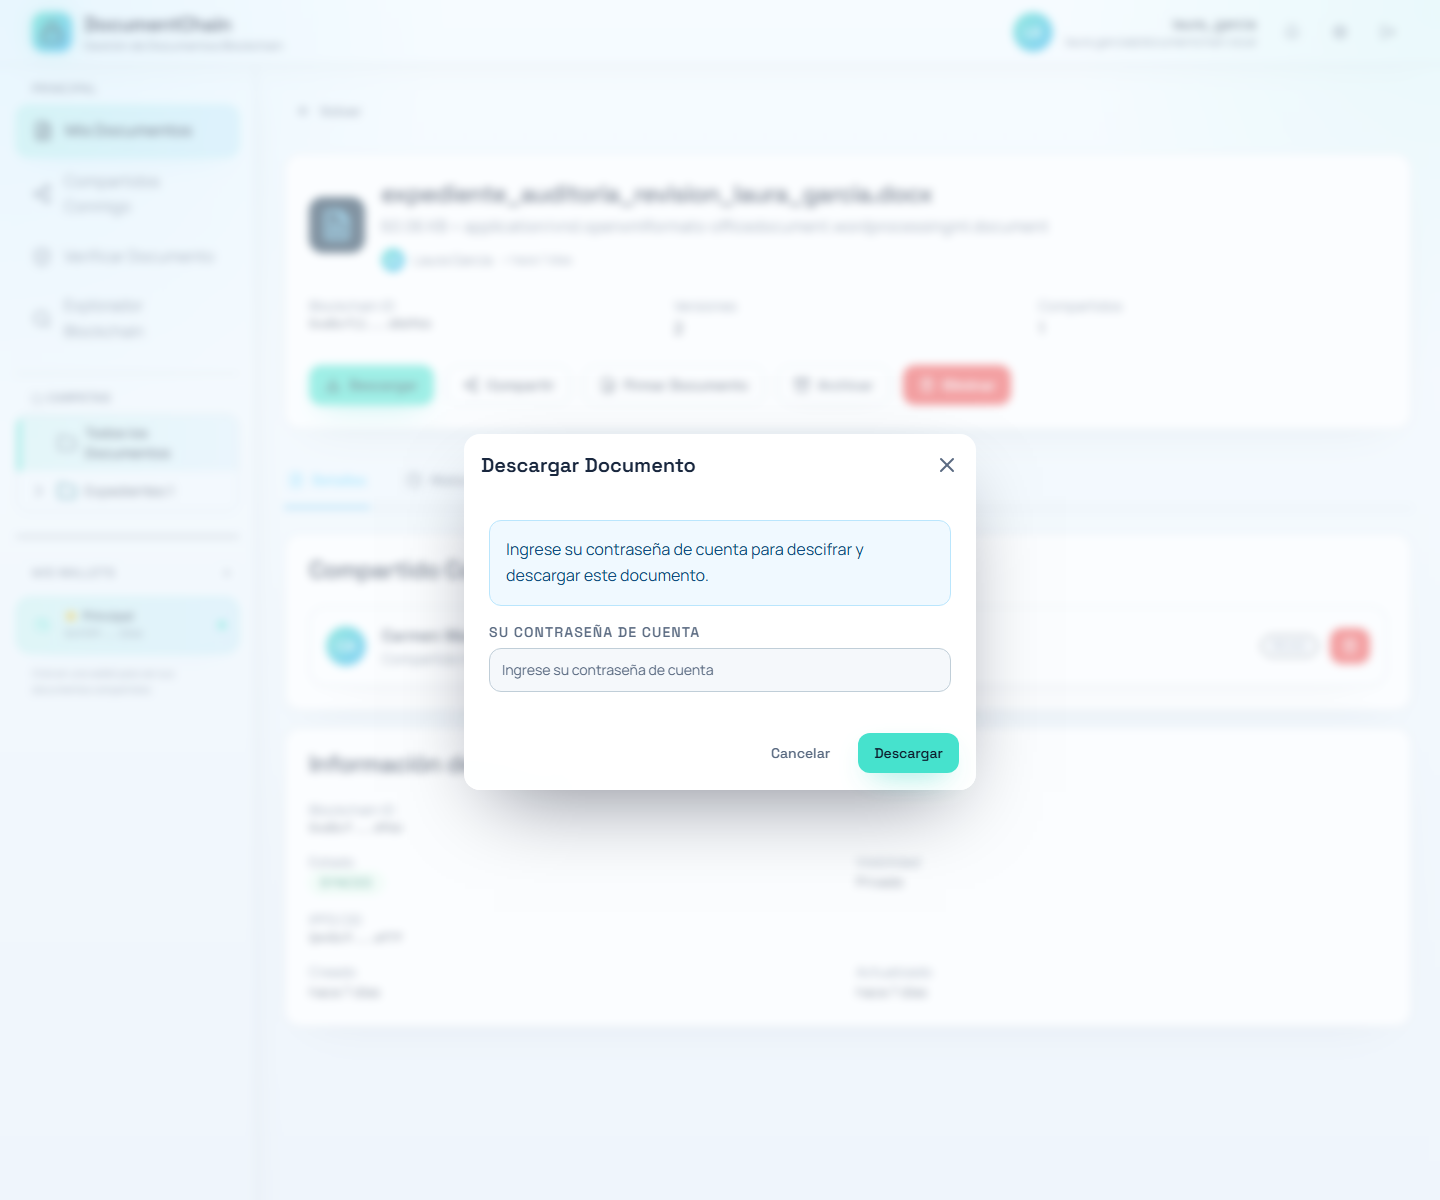
\includegraphics[width=0.75\textwidth]{capturas-ui/download-modal.png}
        \caption{Confirmación de contraseña para descargar}
        \label{fig:download-password}
    \end{figure}
    
    \item Si el documento es privado, introduce tu contraseña y haz clic en \textbf{Confirmar}.
    
    \item En documentos privados, el sistema:
    \begin{enumerate}
        \item Descifra tu clave privada en memoria
        \item Descarga el archivo cifrado de IPFS
        \item Descifra el archivo en tu navegador
        \item Verifica la integridad (checksum SHA-256)
    \end{enumerate}
    
    \item Si el documento es público, la descarga se inicia directamente sin pedir contraseña.

    \item Si la verificación es exitosa, o si se trata de un documento público, el navegador descargará el archivo original.
    
    \item \textbf{Nota}: En documentos privados, el descifrado ocurre en tu navegador. En documentos públicos no se realiza descifrado porque el contenido se ha publicado en claro de forma intencional.
\end{enumerate}

\textbf{Advertencia}: Si introduces una contraseña incorrecta 3 veces, tu sesión se cerrará por seguridad.

\subsubsection{Archivar un documento}

Archivar oculta el documento de las vistas principales sin eliminarlo.

\begin{enumerate}
    \item En la vista de detalles, haz clic en el menú de acciones (tres puntos).
    \item Selecciona \textbf{Archivar}.
    \item Confirma la acción.
    \item El documento desaparecerá de la lista principal y aparecerá en \textbf{Archivados} del sidebar.
\end{enumerate}

Para \textbf{desarchivar}:
\begin{enumerate}
    \item Ve a \textbf{Archivados} en el sidebar.
    \item Abre el documento y selecciona \textbf{Desarchivar}.
\end{enumerate}

\subsubsection{Eliminar un documento}

\textbf{Advertencia}: Eliminar es irreversible a nivel operativo. El sistema marca el documento como eliminado y solicita el desanclado de sus contenidos en IPFS, aunque la desaparición efectiva del contenido depende del garbage collector del nodo o clúster.

\begin{enumerate}
    \item En la vista de detalles, haz clic en el menú de acciones.
    \item Selecciona \textbf{Eliminar}.
    \item El navegador mostrará una confirmación simple para evitar eliminaciones accidentales.
    \item Acepta la confirmación.
    \item El sistema:
    \begin{itemize}
        \item Marcará el documento como eliminado en la base de datos
        \item Solicitará el desanclado en IPFS de los CIDs asociados a sus versiones
        \item Mantendrá intacta la evidencia ya registrada en blockchain
    \end{itemize}
\end{enumerate}

\textbf{Nota}: Si el nodo IPFS todavía no ha ejecutado la recolección de basura, el contenido puede seguir resolviendo durante un tiempo limitado aunque el documento ya no aparezca en la aplicación.

\subsection{Gestión de versiones}

\subsubsection{Crear una nueva versión}

\begin{enumerate}
    \item Abre el documento del que quieres crear una versión.
    \item Ve a la pestaña \textbf{Versiones}.
    \item Haz clic en \textbf{Subir Nueva Versión}.
    \item Se abrirá un modal específico que valida el \textbf{mismo nombre base} y el \textbf{mismo tipo MIME} del documento original.
    \item Sube el nuevo archivo y añade, si lo deseas, un comentario descriptivo.
    \item Pulsa \textbf{Subir y Firmar} y selecciona la wallet con la que registrarás la operación.
    \item Tras la confirmación on-chain, la nueva versión aparecerá en el historial y quedará disponible para activarse como versión operativa.
\end{enumerate}

\begin{figure}[H]
    \centering
    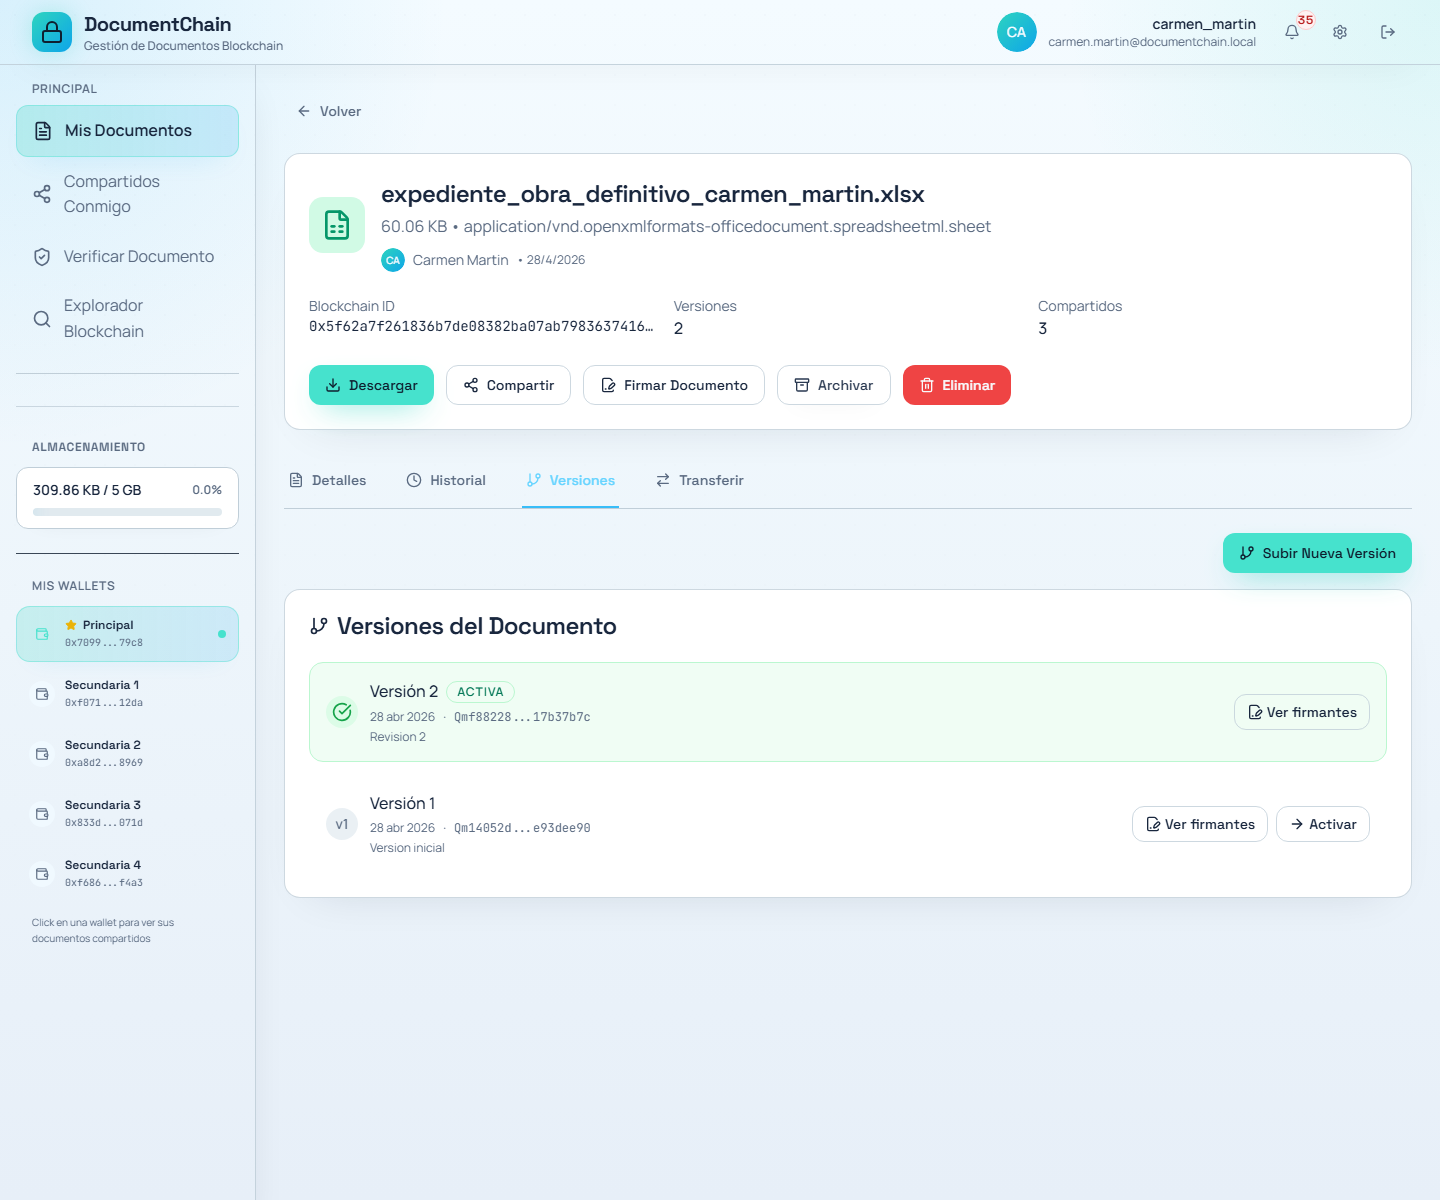
\includegraphics[width=0.95\textwidth]{capturas-ui/versions-tab.png}
    \caption{Pestaña de versiones con historial y acceso a firmantes}
    \label{fig:versions-tab}
\end{figure}

\begin{figure}[H]
    \centering
    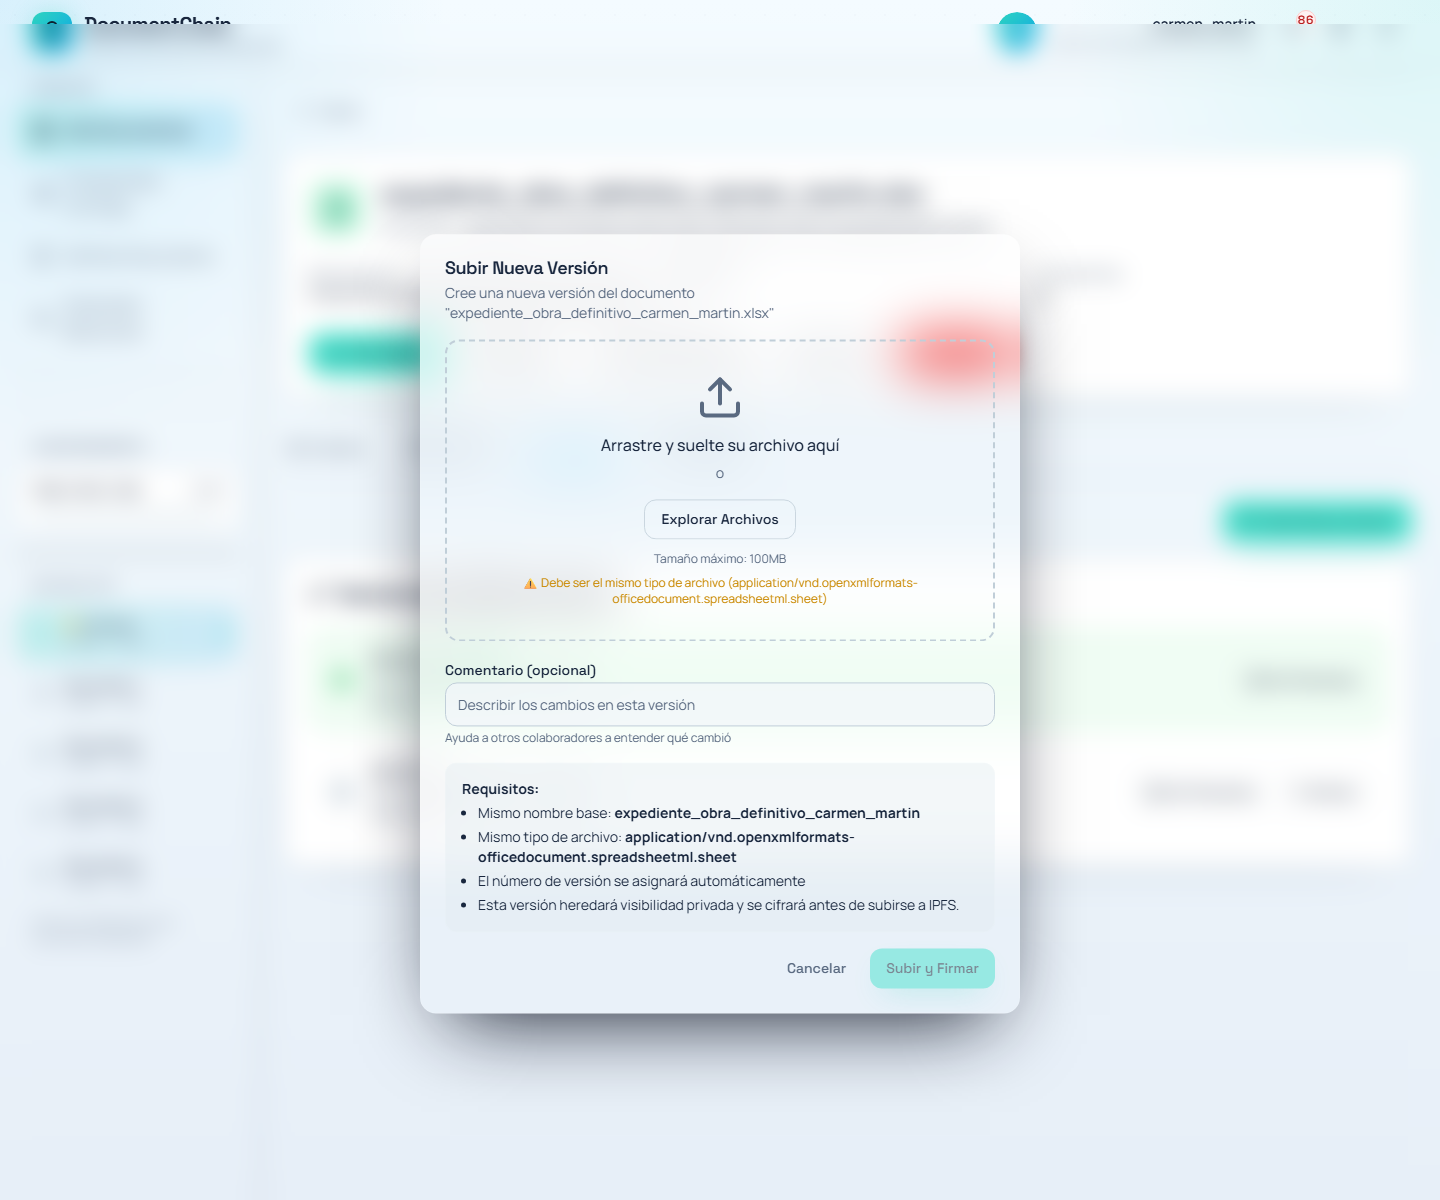
\includegraphics[width=0.82\textwidth]{capturas-ui/upload-version-modal.png}
    \caption{Modal de creación de una nueva versión}
    \label{fig:upload-version-modal}
\end{figure}

\textbf{Consejo}: Usa comentarios descriptivos para facilitar el seguimiento de cambios.

\subsubsection{Consultar el historial de versiones}

\begin{enumerate}
    \item En la pestaña \textbf{Versiones}, cada tarjeta muestra el número de versión, la fecha, el CID abreviado y, si existe, el comentario asociado.
    \item La versión operativa aparece destacada como \textbf{Activa}.
    \item Desde esa misma lista puedes consultar firmantes y, si eres propietario, activar otra versión como operativa.
\end{enumerate}

\subsubsection{Restaurar una versión anterior}

\begin{enumerate}
    \item En el historial de versiones, localiza la versión que deseas restaurar.
    \item Pulsa \textbf{Activar} en la tarjeta de esa versión.
    \item El sistema actualiza el historial y esa versión pasa a ser la \textit{versión operativa} (la que se descarga por defecto).
\end{enumerate}

\textbf{Nota}: Restaurar no elimina las versiones posteriores, solo cambia cuál es la "actual".

\subsection{Firmas digitales}

\subsubsection{Firmar un documento}

\begin{enumerate}
    \item Abre el documento que deseas firmar.
    \item Haz clic en el botón \textbf{Firmar Documento}.
    \item Se abrirá un modal de confirmación.
    
    \begin{figure}[H]
        \centering
        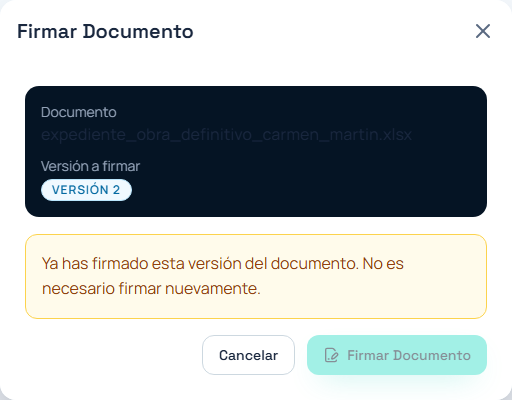
\includegraphics[width=0.75\textwidth]{capturas-ui/sign-modal.png}
        \caption{Modal de firma de documento}
        \label{fig:sign-modal}
    \end{figure}
    
    \item Revisa:
    \begin{itemize}
        \item Nombre del documento
        \item Versión actual a firmar
        \item Comentario opcional asociado a la firma
    \end{itemize}
    
    \item Haz clic en \textbf{Firmar Documento}.
    
    \item El sistema solicitará seleccionar una wallet. Antes de firmar, la wallet mostrará un mensaje legible con el título del documento, la versión y la dirección del contrato, para que sepas exactamente qué estás suscribiendo.
    
    \item Confirma la transacción en tu wallet y espera a que se mine.
    
    \item Verás una notificación de éxito y el evento quedará reflejado en el historial del documento y en la auditoría blockchain.
\end{enumerate}

\textbf{Nota}: La firma se registra on-chain con tu dirección de wallet y el timestamp del bloque, proporcionando no-repudio criptográfico. El mensaje legible que aparece en la wallet es generado por el backend y no puede ser alterado por el frontend.

\subsubsection{Consultar los firmantes de una versión}

\begin{enumerate}
    \item Abre el documento y entra en la pestaña \textbf{Versiones}.
    \item Localiza la versión que quieras revisar.
    \item Pulsa \textbf{Ver firmantes}.
    \item El sistema abrirá un modal con la lista de firmas registradas para esa versión.
    \item Selecciona cualquiera de los firmantes para ver su ficha resumida.
    \item En esa ficha se muestran el avatar, el nombre visible, el alias disponible, la wallet utilizada para la firma, la fecha registrada y el estado de sincronización blockchain.
    \item Si la cuenta original ya no está disponible, la aplicación seguirá mostrando la identidad histórica conservada junto a la firma.
\end{enumerate}

\begin{figure}[H]
    \centering
    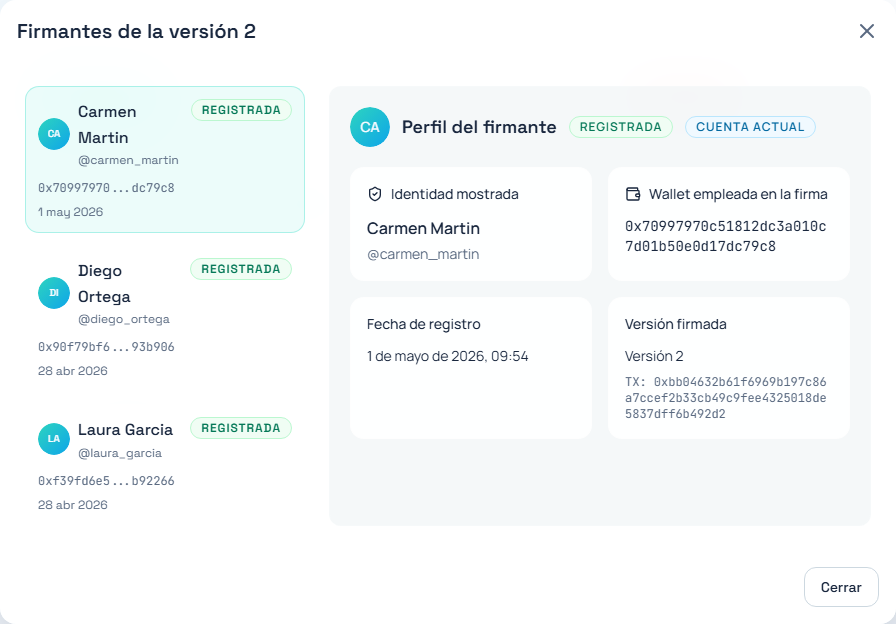
\includegraphics[width=0.82\textwidth]{capturas-ui/signers-modal.png}
    \caption{Ficha resumida del firmante de una versión}
    \label{fig:signers-modal}
\end{figure}

La comprobación detallada de la validez blockchain continúa disponible desde las vistas públicas de verificación y desde la transacción asociada cuando proceda.

\subsection{Compartir documentos}

\subsubsection{Compartir con otro usuario}

\begin{enumerate}
    \item Abre el documento que deseas compartir.
    \item Haz clic en el botón \textbf{Compartir} (icono de personas o link).
    \item Se abrirá un modal con opciones de compartición.
    
    \begin{figure}[H]
        \centering
        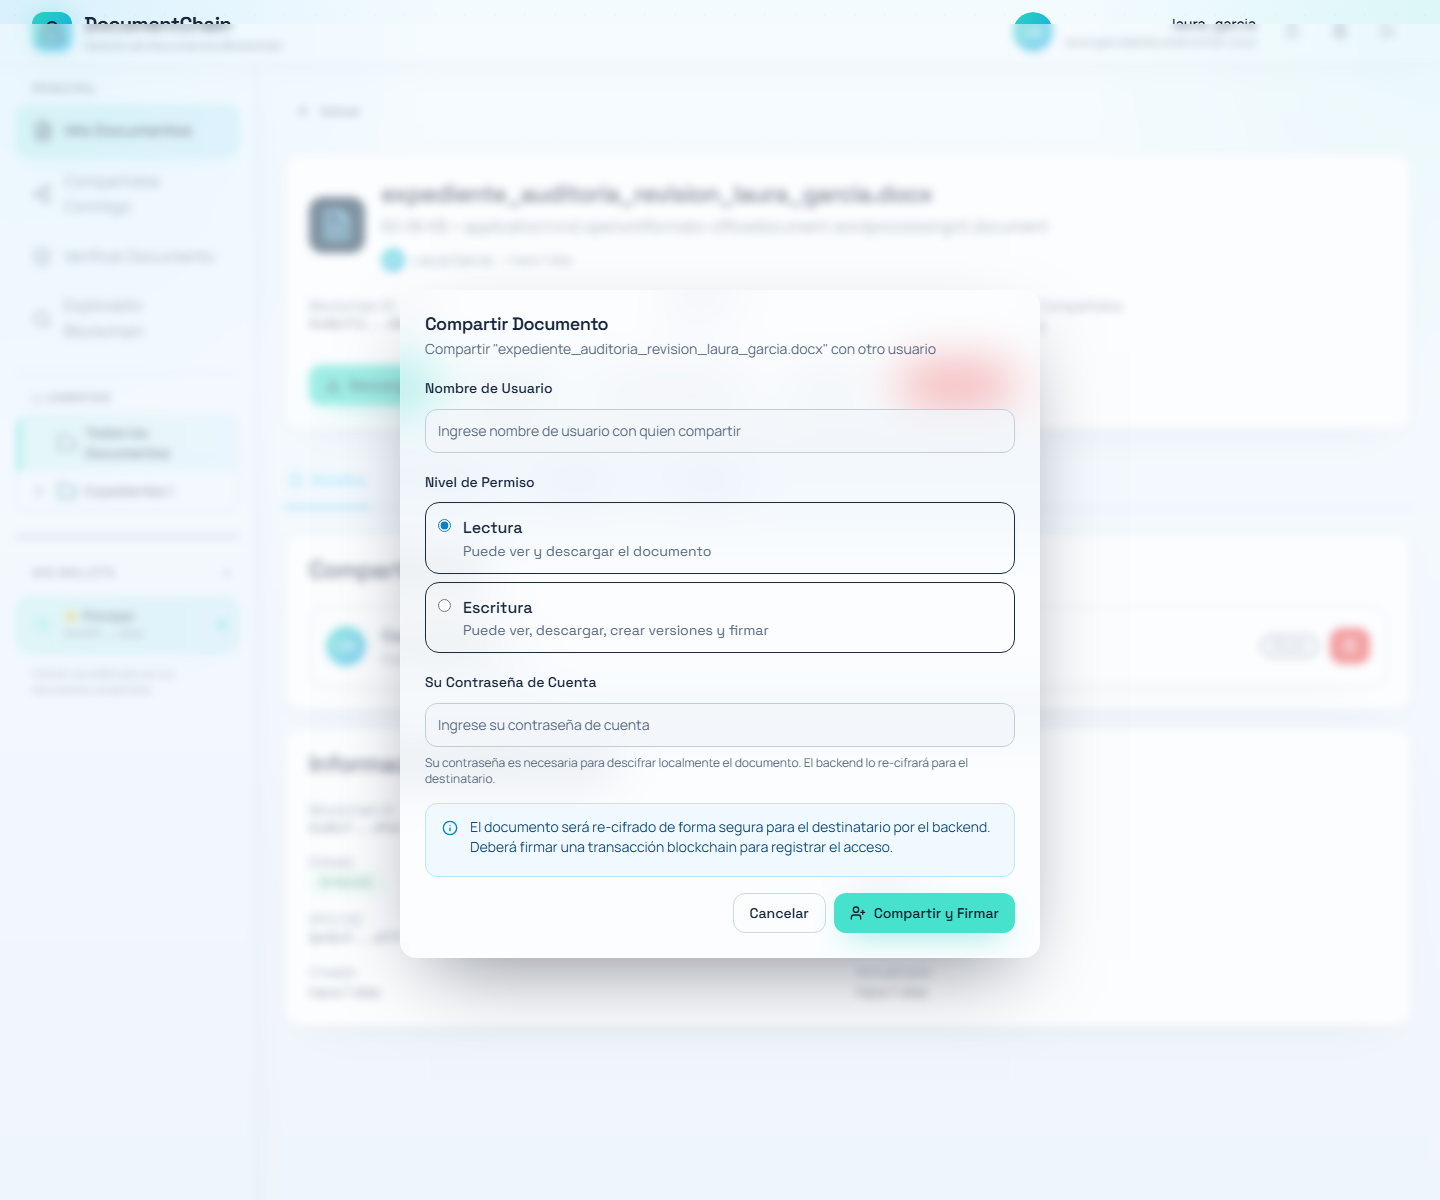
\includegraphics[width=0.78\textwidth]{capturas-ui/share-modal.png}
        \caption{Modal de compartición de documento}
        \label{fig:share-modal}
    \end{figure}
    
    \item En el campo \textbf{Nombre de Usuario}, escribe el identificador del destinatario.
    \item Elige el rol que tendrá:
    \begin{itemize}
        \item \textbf{Lectura}: permite ver y descargar el documento
        \item \textbf{Escritura}: permite ver, descargar, crear versiones y firmar
    \end{itemize}
    
    \item Se te solicitará tu contraseña (para descifrar tu clave privada y re-encriptar la clave del documento).
    
    \item Introduce tu contraseña y haz clic en \textbf{Compartir y Firmar}.
    
    \item El sistema re-encriptará la clave simétrica del documento con la clave pública del destinatario.
    
    \item El sistema solicitará una wallet para firmar la transacción blockchain correspondiente.
    
    \item Una vez confirmada, el usuario aparecerá en la lista de accesos compartidos del detalle, mostrando su avatar si lo tiene configurado.
    
    \item El destinatario recibirá una notificación in-app y por email.
\end{enumerate}

\textbf{Nota}: El proceso de re-cifra garantiza que cada usuario compartido recibe una clave simétrica protegida para su propia clave privada, sin necesidad de volver a exponer el archivo original.


\subsubsection{Acceder a documentos compartidos contigo}

\begin{enumerate}
    \item Accede a \texttt{/app/shared} desde la barra lateral mediante la entrada \textbf{Compartidos Conmigo}.
    \item La vista mostrará únicamente los documentos asociados a la \textbf{wallet activa} del usuario.
    \item Puedes buscar por nombre y filtrar por tipo de archivo.
    \item Cada tarjeta indica el propietario del documento y, cuando procede, las etiquetas asociadas.
    \item Si cambias la wallet activa, el listado se actualizará para reflejar los accesos compartidos con esa dirección concreta.
\end{enumerate}

\begin{figure}[H]
    \centering
    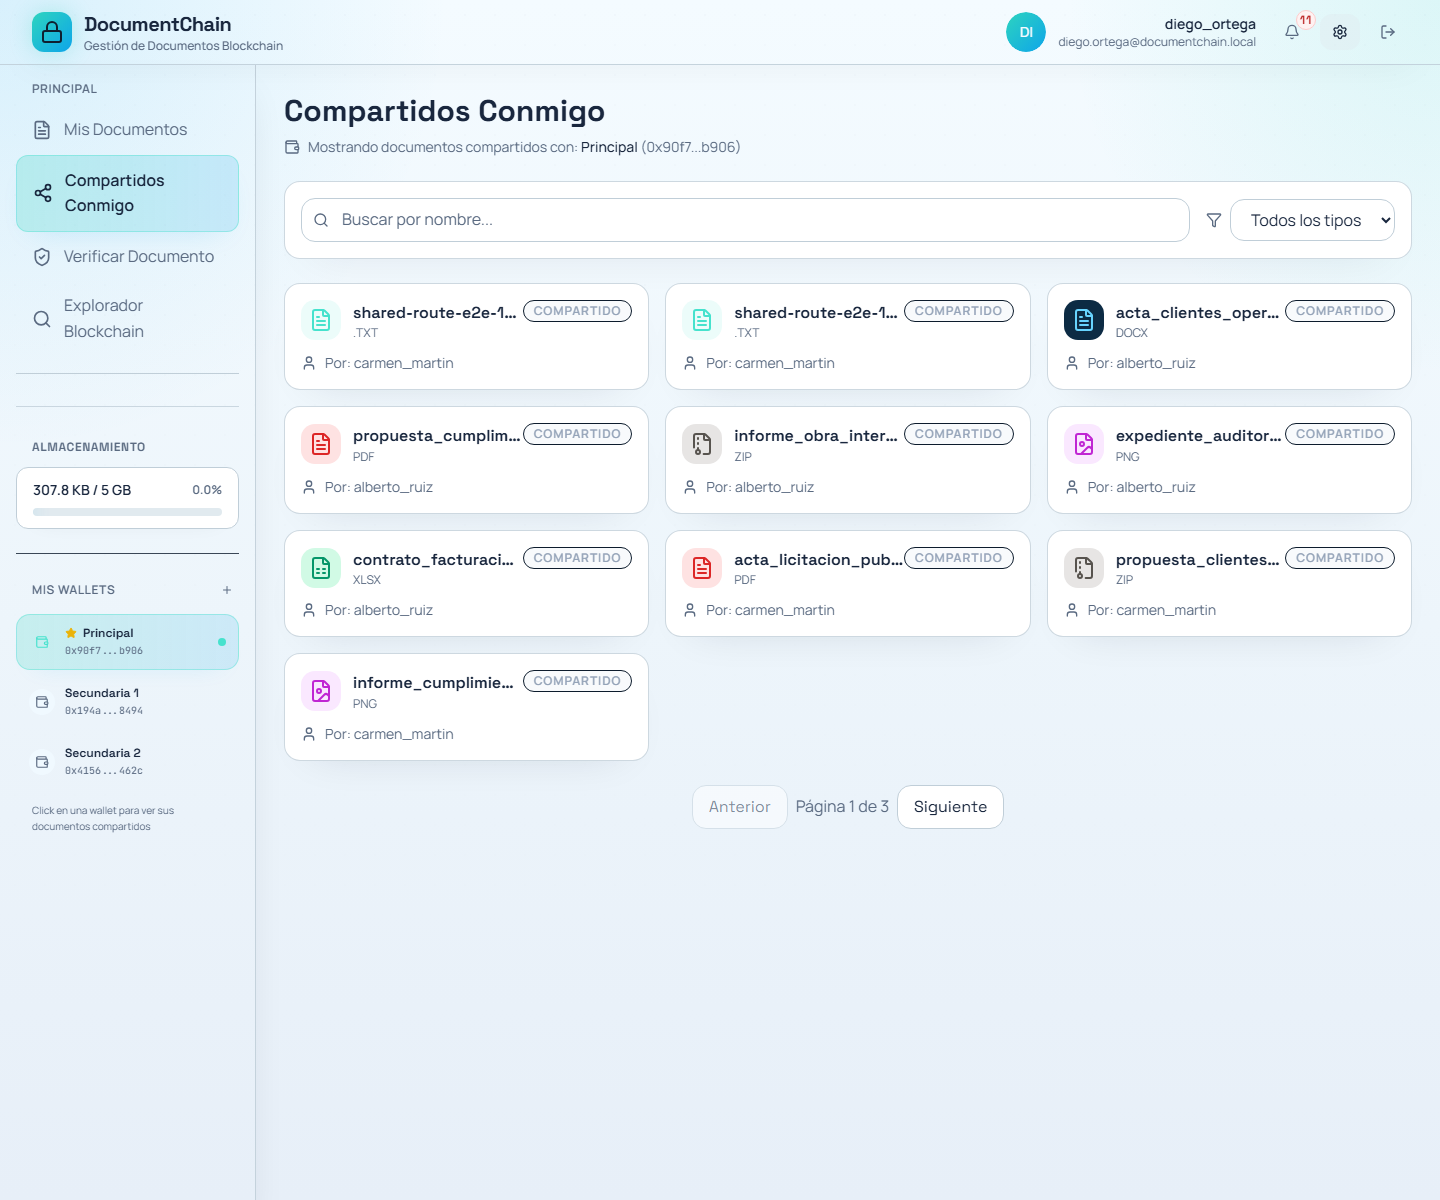
\includegraphics[width=0.95\textwidth]{capturas-ui/shared-page.png}
    \caption{Vista de documentos compartidos con la wallet activa (escritorio)}
    \label{fig:shared-page}
\end{figure}

\begin{figure}[H]
    \centering
    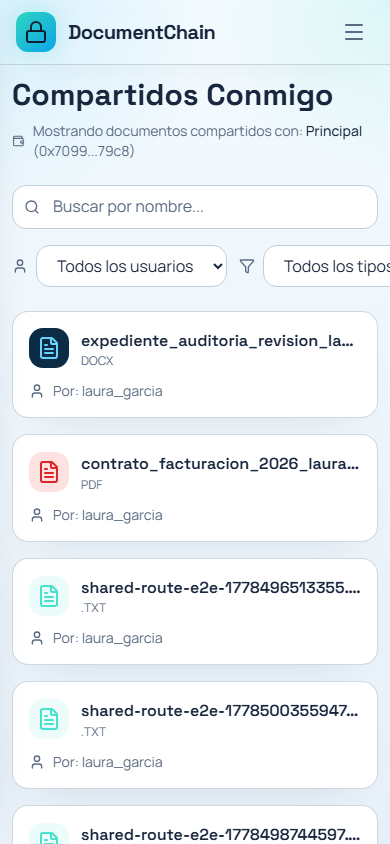
\includegraphics[width=0.45\textwidth]{capturas-ui/mobile-shared-documents.png}
    \caption{Vista de documentos compartidos con la wallet activa (móvil)}
    \label{fig:shared-page-mobile}
\end{figure}

En la versión entregada no existe todavía una acción directa para cambiar el rol de un usuario ya compartido. Si es necesario pasar de lectura a escritura, o al revés, el procedimiento disponible consiste en \textbf{revocar} primero el acceso actual y volver a \textbf{compartir} después el documento con el nuevo nivel.

\subsubsection{Revocar acceso}

\begin{enumerate}
    \item Abre el documento y, dentro de \textbf{Detalles}, localiza el bloque \textbf{Compartido con}.
    \item Haz clic en el icono \textbf{X} o \textbf{Revocar} junto al usuario.
    \item Confirma la acción.
    \item Confirma la firma con la wallet seleccionada.
    \item El usuario perderá acceso on-chain inmediatamente.
    \item Sin embargo, si ya descargó el documento, conservará la copia descifrada localmente.
\end{enumerate}

\textcolor{orange}{\textbf{Importante}}: La revocación impide futuras descargas, pero no borra copias ya descargadas.

\subsubsection{Transferir propiedad}

Solo el OWNER puede transferir la propiedad:

\begin{enumerate}
    \item Abre el detalle del documento y entra en la pestaña \textbf{Transferir}.
    \item Busca al nuevo propietario por nombre de usuario; los resultados muestran el avatar de cada usuario cuando está disponible.
    \item Introduce la contraseña de tu cuenta para descifrar localmente la clave del documento.
    \item El sistema preparará la transferencia y te solicitará la wallet principal para firmar la transacción blockchain.
    \item \textbf{Advertencia}: la operación es irreversible; una vez confirmada, el nuevo propietario pasará a controlar el documento y tú abandonarás el rol OWNER.
\end{enumerate}

\begin{figure}[H]
    \centering
    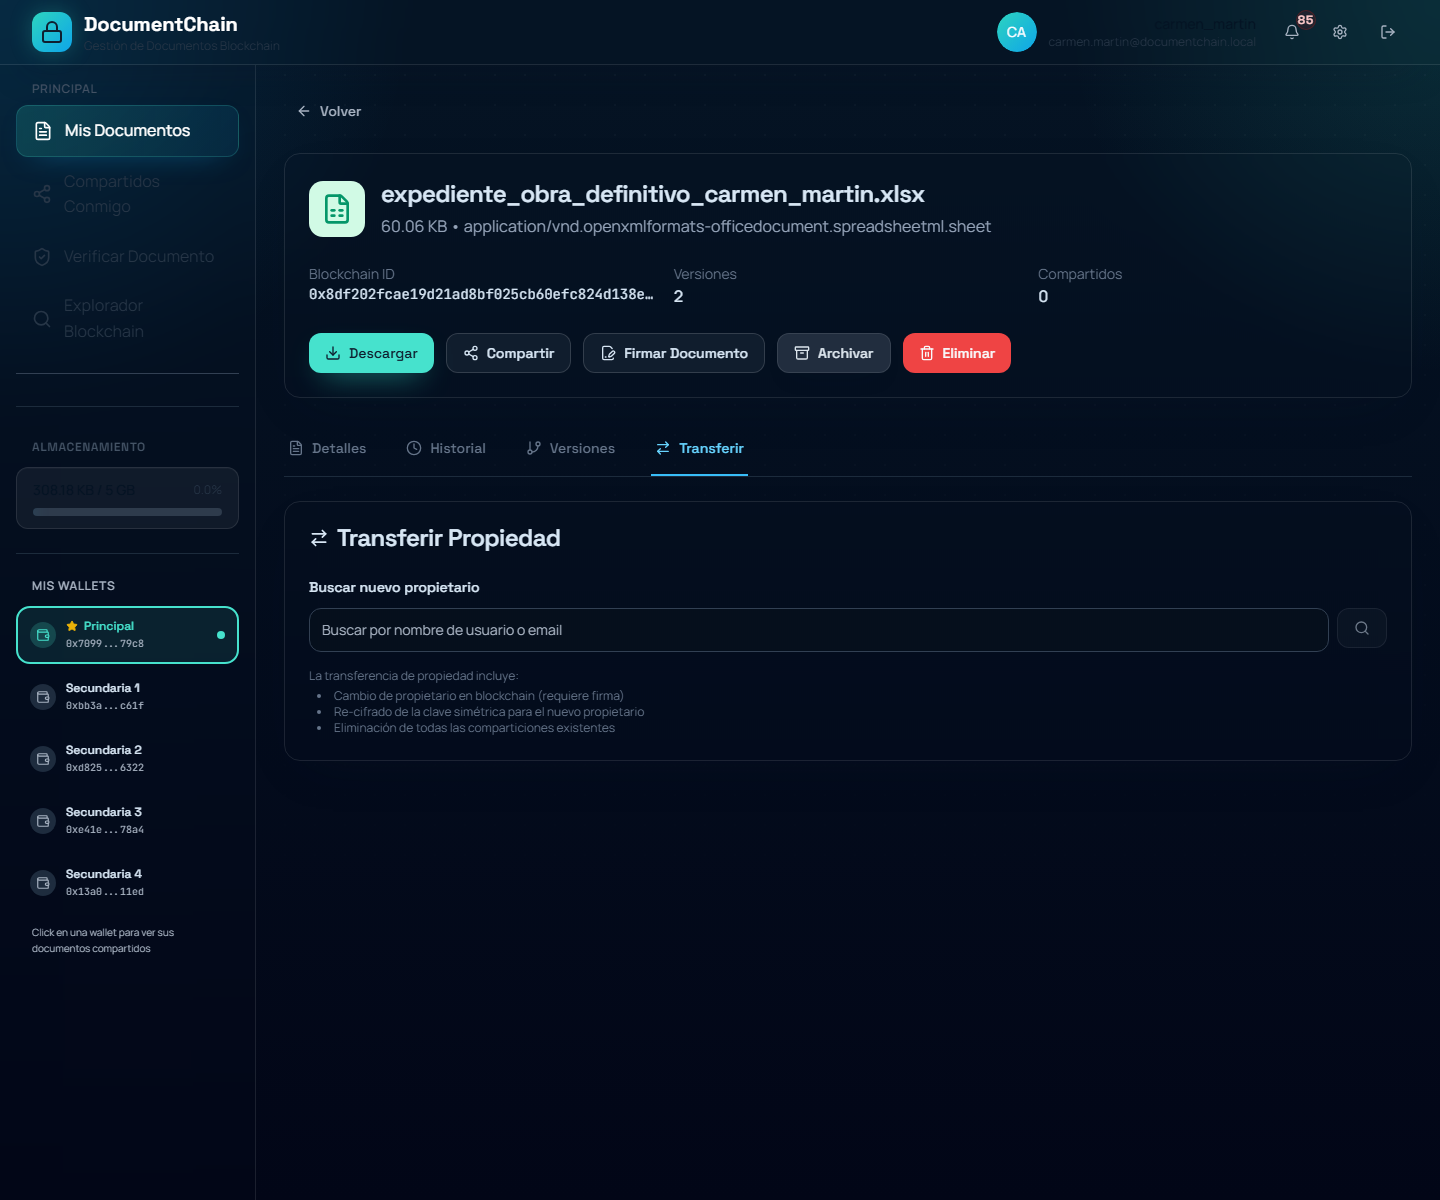
\includegraphics[width=0.95\textwidth]{capturas-ui/transfer-tab.png}
    \caption{Pestaña de transferencia de propiedad del documento}
    \label{fig:transfer-tab}
\end{figure}

\subsection{Organización: Carpetas y clasificación}

\subsubsection{Crear una carpeta}

\begin{enumerate}
    \item En el sidebar, haz clic en el botón \textbf{+} junto a \textbf{Carpetas}.
    \item Introduce el nombre de la carpeta.
    \item (Opcional) Añade descripción, selecciona color e icono.
    \item Si quieres crear una subcarpeta, selecciona la carpeta padre.
    \item Haz clic en \textbf{Crear}.
\end{enumerate}

\begin{figure}[H]
    \centering
    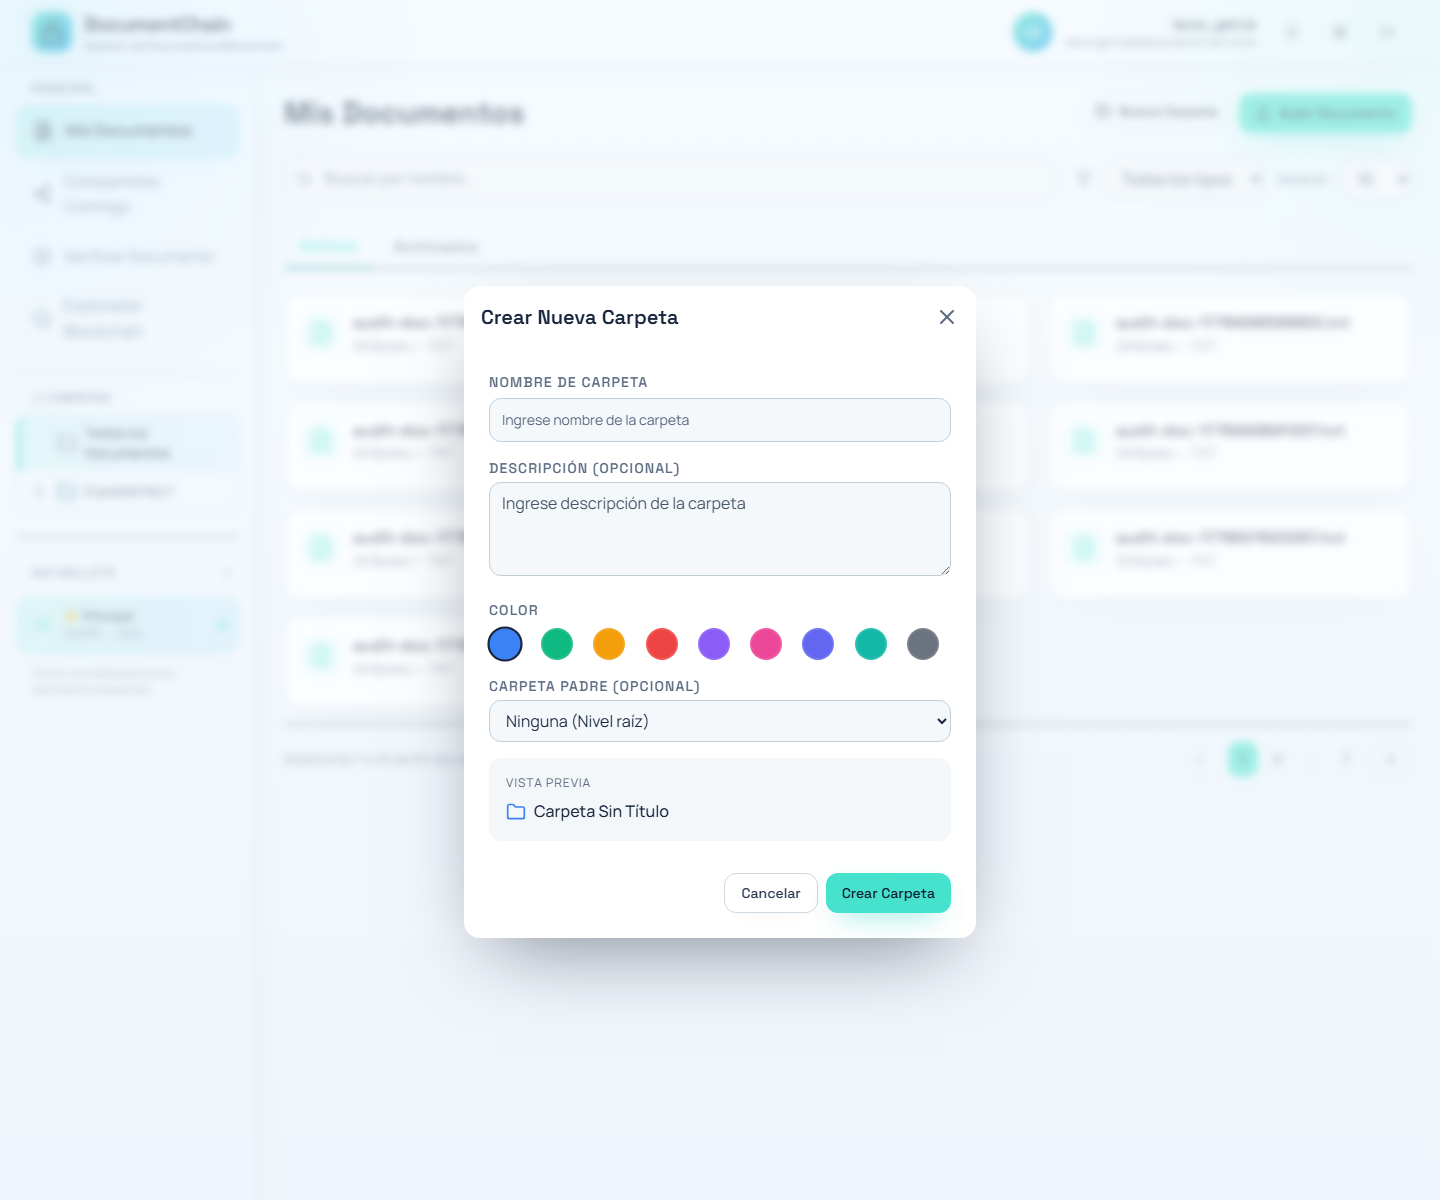
\includegraphics[width=0.82\textwidth]{capturas-ui/create-folder-modal.png}
    \caption{Modal de creación de carpeta}
    \label{fig:create-folder}
\end{figure}

La clasificación complementaria se realiza durante la subida o la creación de nuevas versiones, donde es posible asociar \textbf{carpeta} y \textbf{etiquetas} para facilitar búsquedas posteriores.

\subsubsection{Clasificar con etiquetas}

\begin{enumerate}
    \item Durante la subida de un documento o la publicación de una nueva versión, utiliza el campo \textbf{Etiquetas} del formulario.
    \item Las etiquetas admiten varios términos separados por comas y mejoran la búsqueda posterior.
    \item Una vez guardado el documento, esos metadatos aparecerán también en la vista de detalle y en los resultados de búsqueda.
\end{enumerate}

\subsection{Timeline y auditoría}

\subsubsection{Ver timeline de un documento}

\begin{enumerate}
    \item Abre el documento.
    \item Ve a la pestaña \textbf{Historial}.
    \item Verás un historial cronológico de todos los eventos:
    \begin{itemize}
        \item Creación
        \item Nuevas versiones
        \item Firmas
        \item Comparticiones y cambios de permisos
        \item Transferencias
        \item Descargas
    \end{itemize}
\end{enumerate}

\begin{figure}[H]
    \centering
    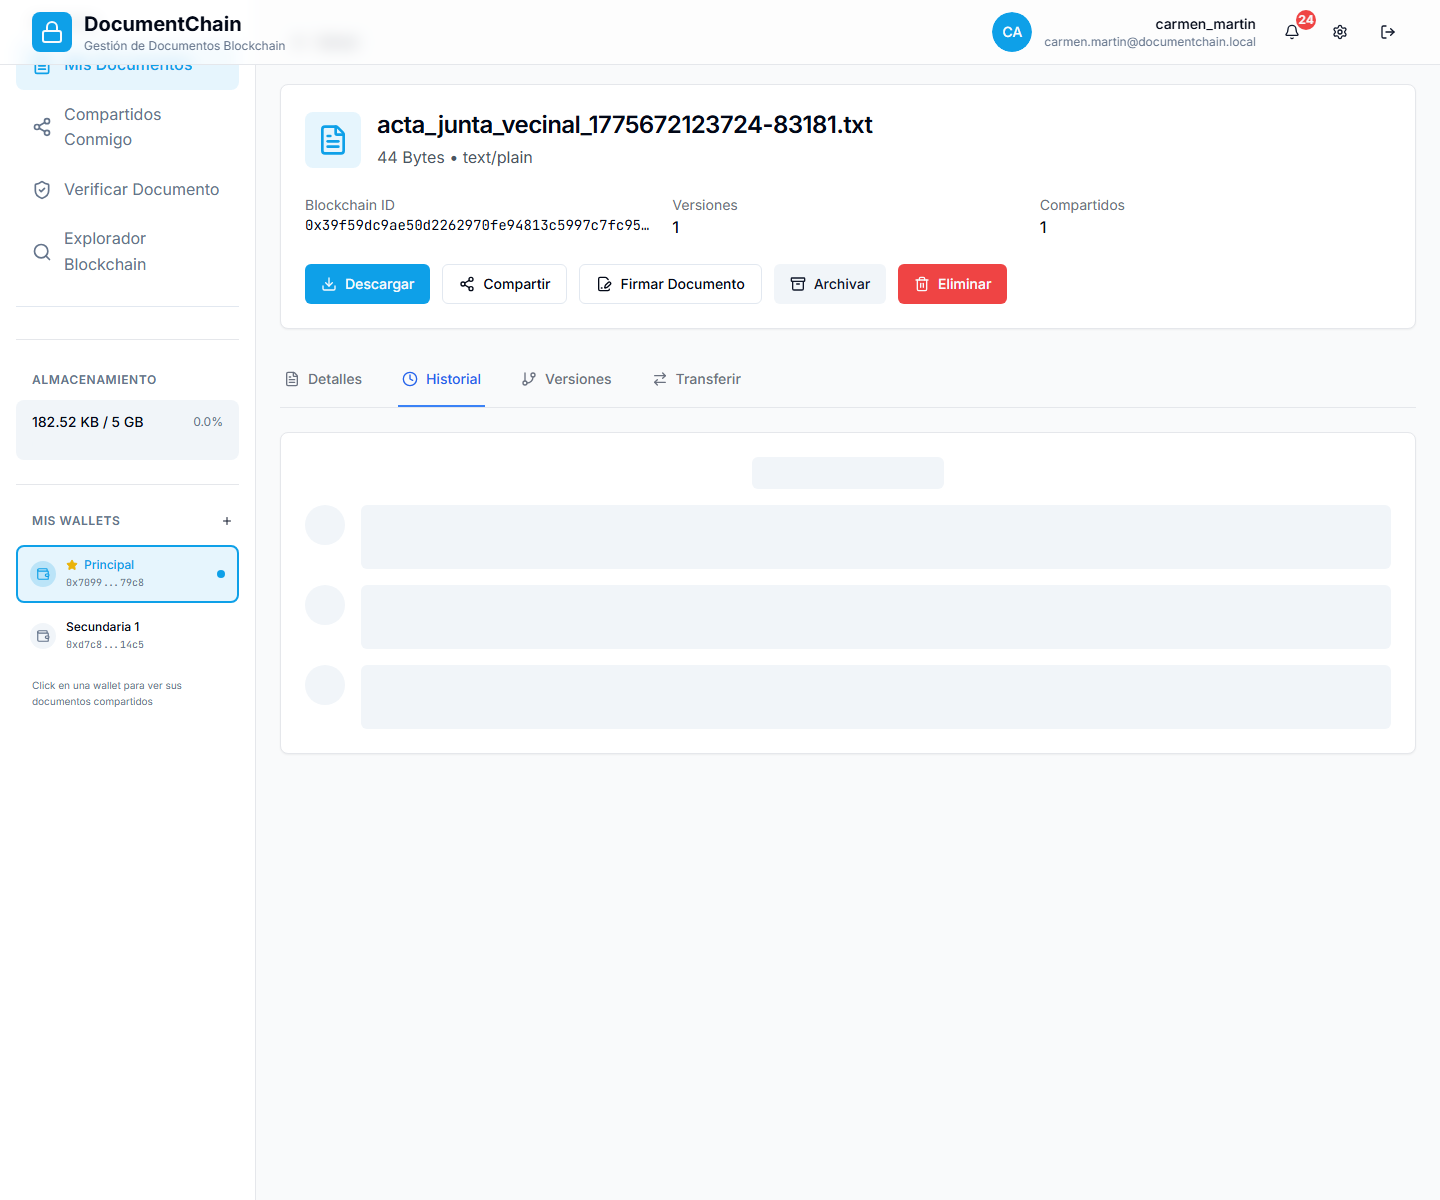
\includegraphics[width=0.95\textwidth]{capturas-ui/timeline-page.png}
    \caption{Historial cronológico del documento}
    \label{fig:timeline}
\end{figure}

\subsection{Verificación documental y auditoría pública}

\subsubsection{Verificar un documento desde la aplicación}

\begin{enumerate}
    \item Accede a \texttt{/app/verify} desde la barra lateral.
    \item Elige el método de verificación: archivo original, CID de IPFS o identificador blockchain.
    \item Introduce el dato correspondiente y pulsa \textbf{Verificar Documento}.
    \item La interfaz mostrará si el documento existe, si coincide con el registro blockchain y qué metadatos principales tiene asociados.
\end{enumerate}

\begin{figure}[H]
    \centering
    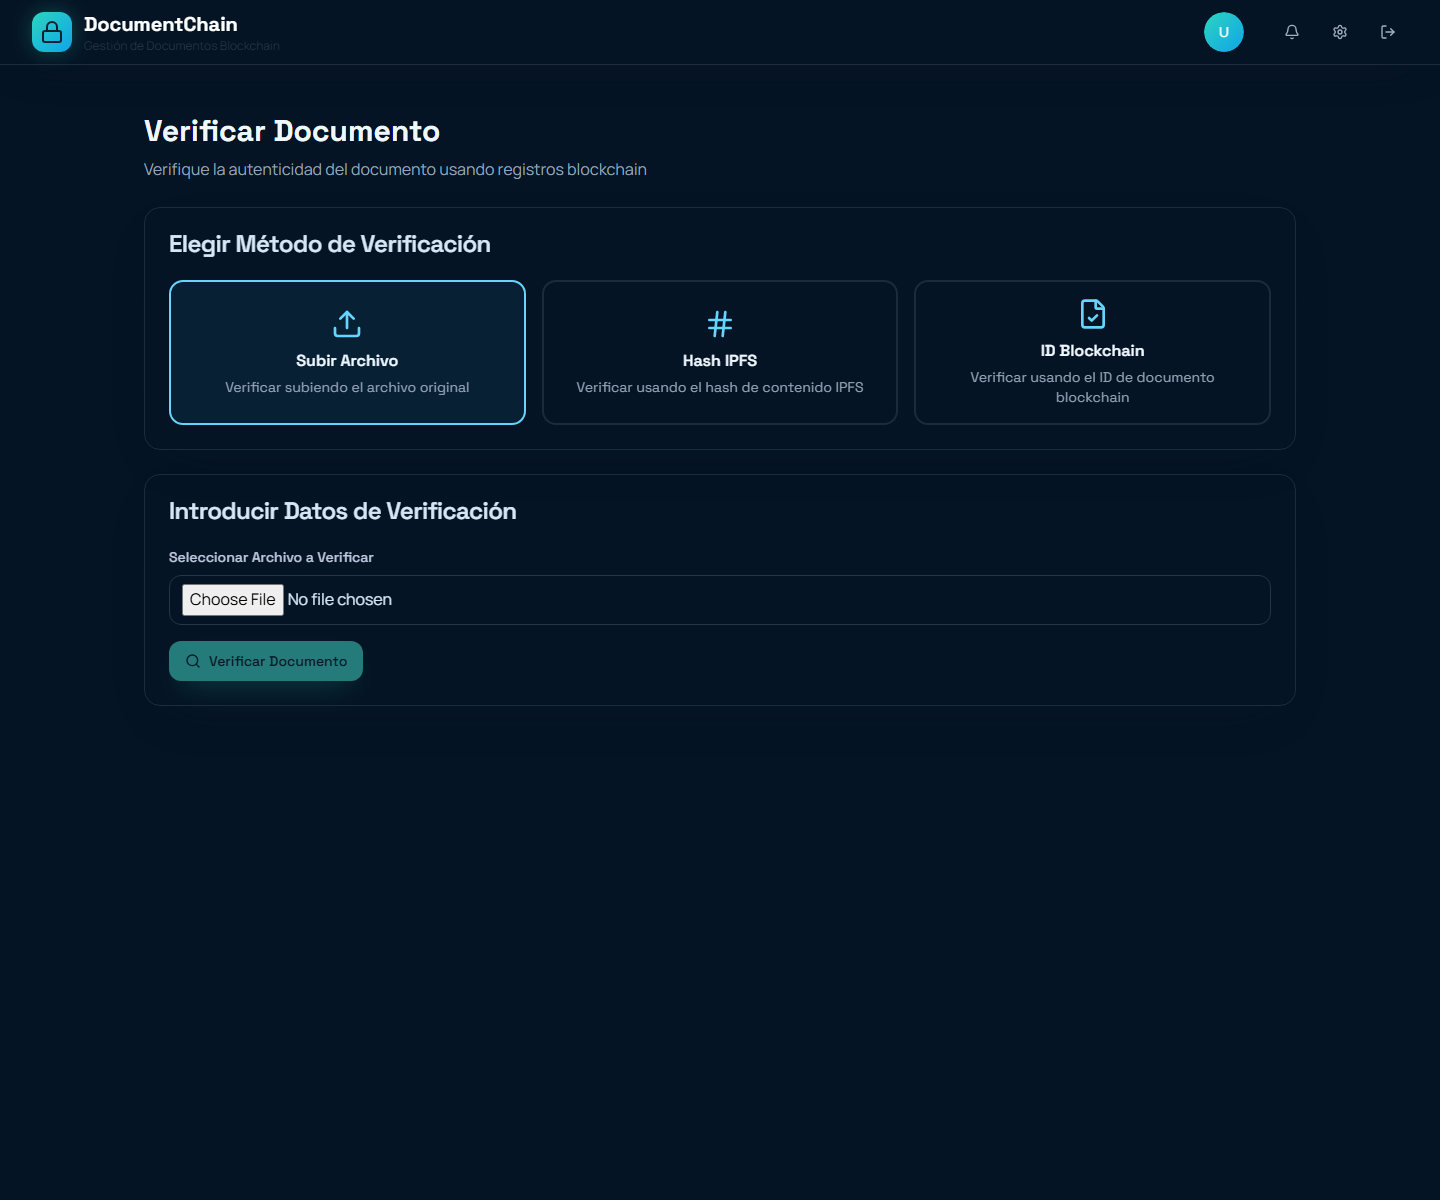
\includegraphics[width=0.95\textwidth]{capturas-ui/verify-page.png}
    \caption{Página de verificación pública de documentos (escritorio)}
    \label{fig:verify-page}
\end{figure}

\begin{figure}[H]
    \centering
    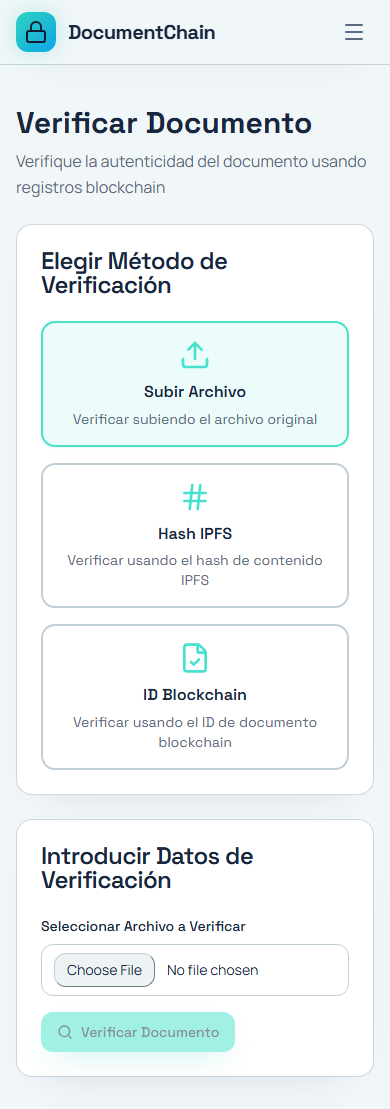
\includegraphics[width=0.45\textwidth]{capturas-ui/mobile-verify.png}
    \caption{Página de verificación pública de documentos (móvil)}
    \label{fig:verify-page-mobile}
\end{figure}

\subsubsection{Consultar la auditoría pública}

\begin{enumerate}
    \item Accede a \texttt{/audit} sin necesidad de iniciar sesión.
    \item La página pública permite consultar trazas blockchain, estadísticas agregadas e información de integridad sin exponer contenido privado.
    \item Esta vista resulta útil para auditorías externas y para comprobaciones rápidas por parte de terceros.
\end{enumerate}

\begin{figure}[H]
    \centering
    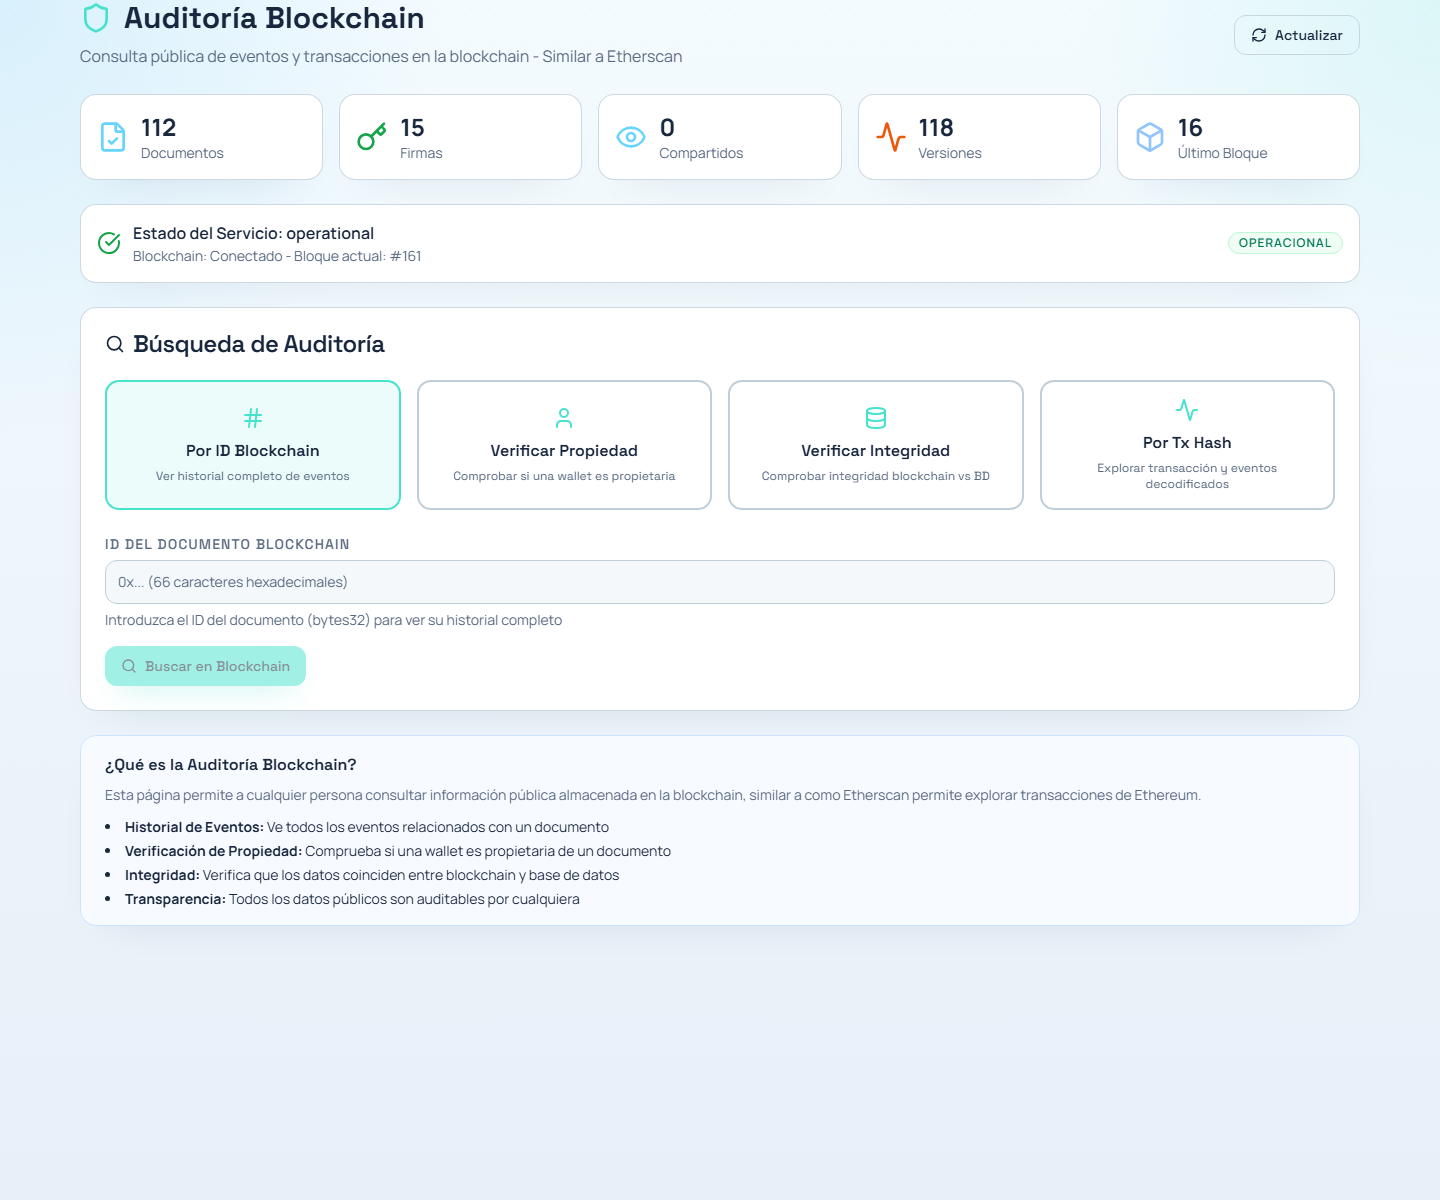
\includegraphics[width=0.95\textwidth]{capturas-ui/public-audit-page.png}
    \caption{Vista pública de auditoría blockchain}
    \label{fig:public-audit-page}
\end{figure}

\subsubsection{Consultar un documento público mediante enlace}

\begin{enumerate}
    \item Abre la URL pública del documento, normalmente con el formato \path{/public/d/:publicId}.
    \item Si necesitas una versión concreta, añade el sufijo \path{/v/:versionNumber} al enlace público del documento.
    \item La página mostrará una previsualización del contenido, sus metadatos básicos y el listado de versiones públicas disponibles.
    \item Desde esa misma vista puedes descargar el documento directamente sin iniciar sesión.
    \item Si el documento tiene varias versiones públicas, selecciona la deseada en el panel lateral para abrir la ruta específica de esa versión.
    \item En la parte inferior también se muestran las firmas registradas y el historial público asociado al documento.
    \item Si necesitas continuar en el entorno autenticado para firmar o revisar más detalles, utiliza \textbf{Abrir en la aplicación} o \textbf{Iniciar sesión y continuar}.
\end{enumerate}

\subsection{Notificaciones}

\subsubsection{Ver notificaciones}

\begin{enumerate}
    \item Haz clic en el icono de \textbf{campana} o accede a \texttt{/app/notifications}.
    \item Se abrirá una vista dedicada con las notificaciones recientes.
    \item Las no leídas aparecen resaltadas y pueden marcarse de forma individual o masiva.
    \item Tipos de notificaciones:
    \begin{itemize}
        \item Documento compartido contigo
        \item Nuevo firmante en tu documento
        \item Nueva versión registrada sobre un documento propio o compartido
        \item Permisos modificados
        \item Sincronización blockchain completada
    \end{itemize}
\end{enumerate}

\begin{figure}[H]
    \centering
    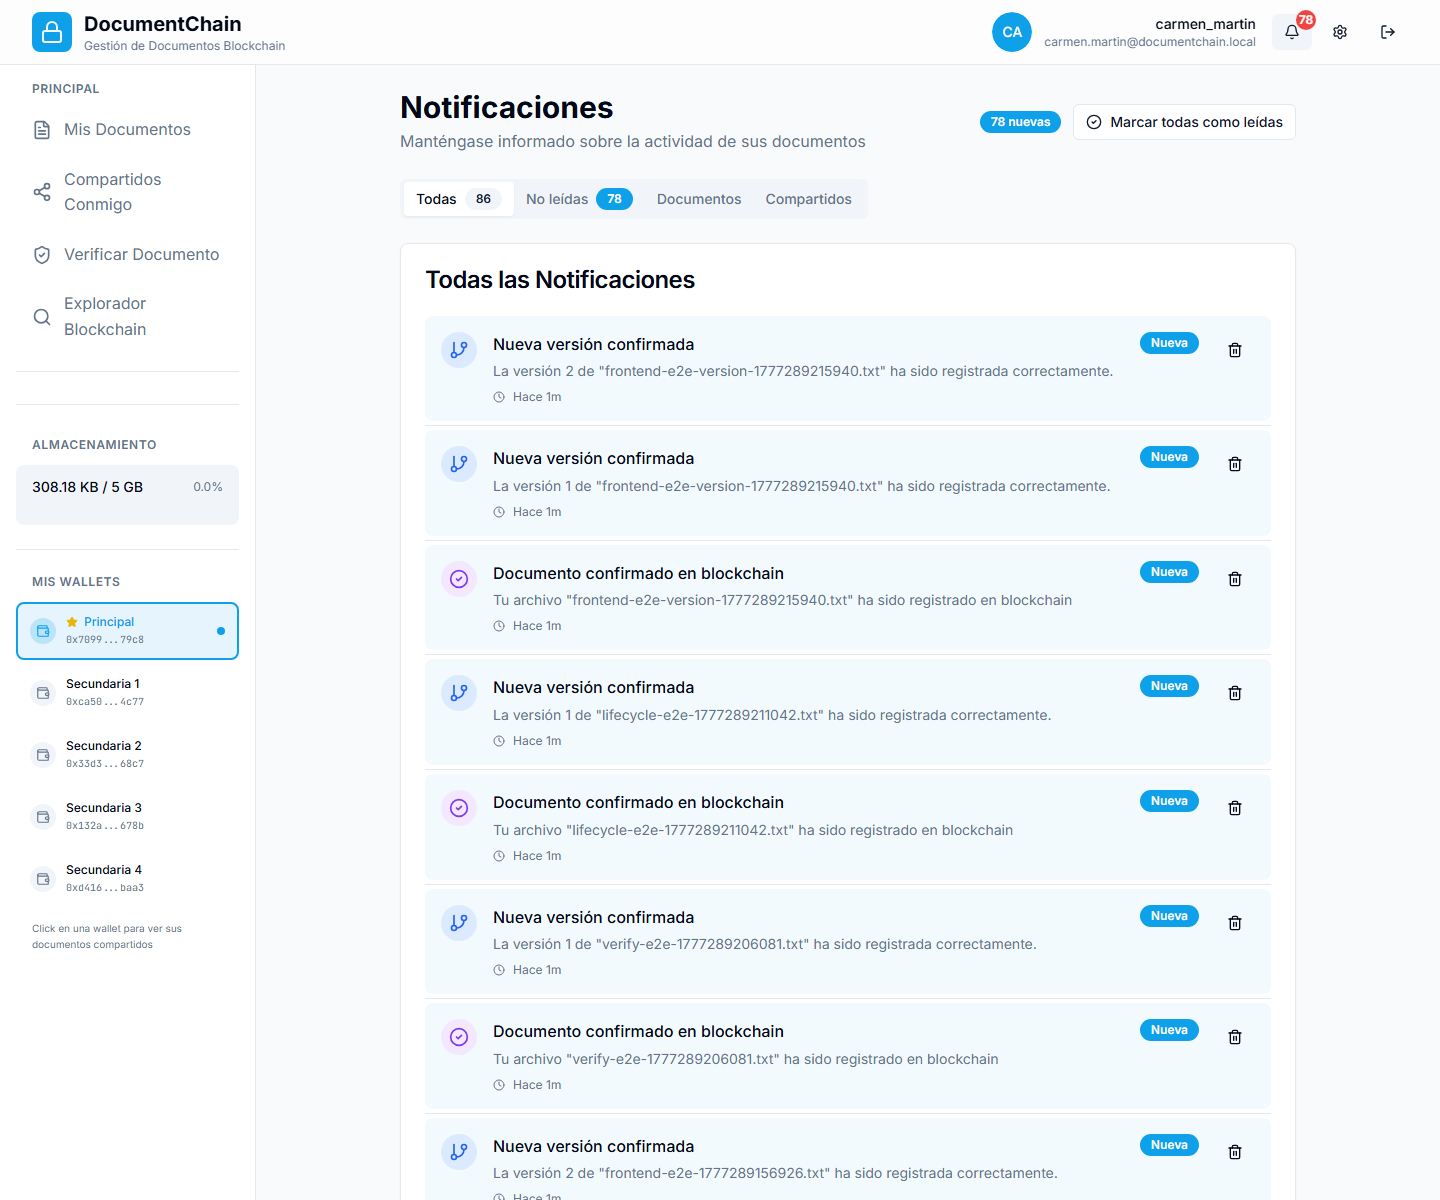
\includegraphics[width=0.95\textwidth]{capturas-ui/notifications-page.png}
    \caption{Centro de notificaciones (escritorio)}
    \label{fig:notifications-page}
\end{figure}

\begin{figure}[H]
    \centering
    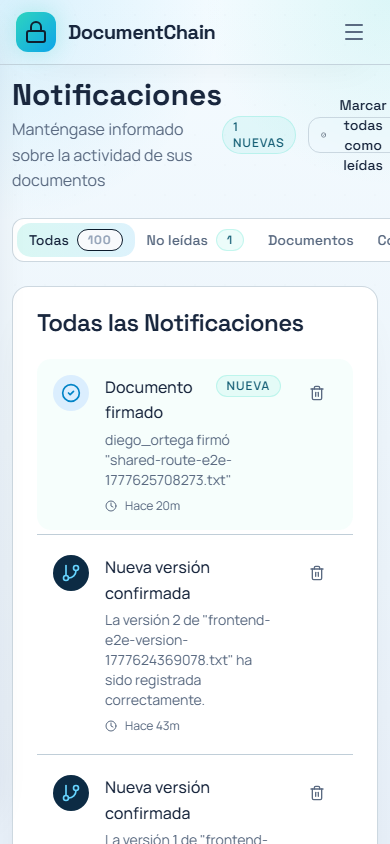
\includegraphics[width=0.45\textwidth]{capturas-ui/mobile-notifications.png}
    \caption{Centro de notificaciones (móvil)}
    \label{fig:notifications-page-mobile}
\end{figure}

\subsubsection{Gestionar notificaciones}

\begin{enumerate}
    \item Usa las pestañas \textbf{Todas}, \textbf{No leídas}, \textbf{Documentos} y \textbf{Compartidos} para filtrar el listado.
    \item Haz clic sobre una notificación no leída para marcarla como leída.
    \item Si deseas limpiar el panel, utiliza \textbf{Marcar todas como leídas}.
    \item Cada entrada incluye además un botón de papelera para eliminarla individualmente.
\end{enumerate}

Cuando un usuario con permisos de edición crea una nueva versión sobre un documento ajeno, el propietario recibe un aviso específico que identifica la operación como una actualización realizada por un editor. De este modo, el panel de notificaciones diferencia entre cambios propios y cambios introducidos por terceros con permisos válidos.

Si se mantienen activadas las notificaciones por email, estos eventos también pueden remitirse por correo. En la figura siguiente se muestra el formato empleado para el aviso de firma de documento, con un acceso directo al recurso afectado.

\begin{figure}[H]
    \centering
    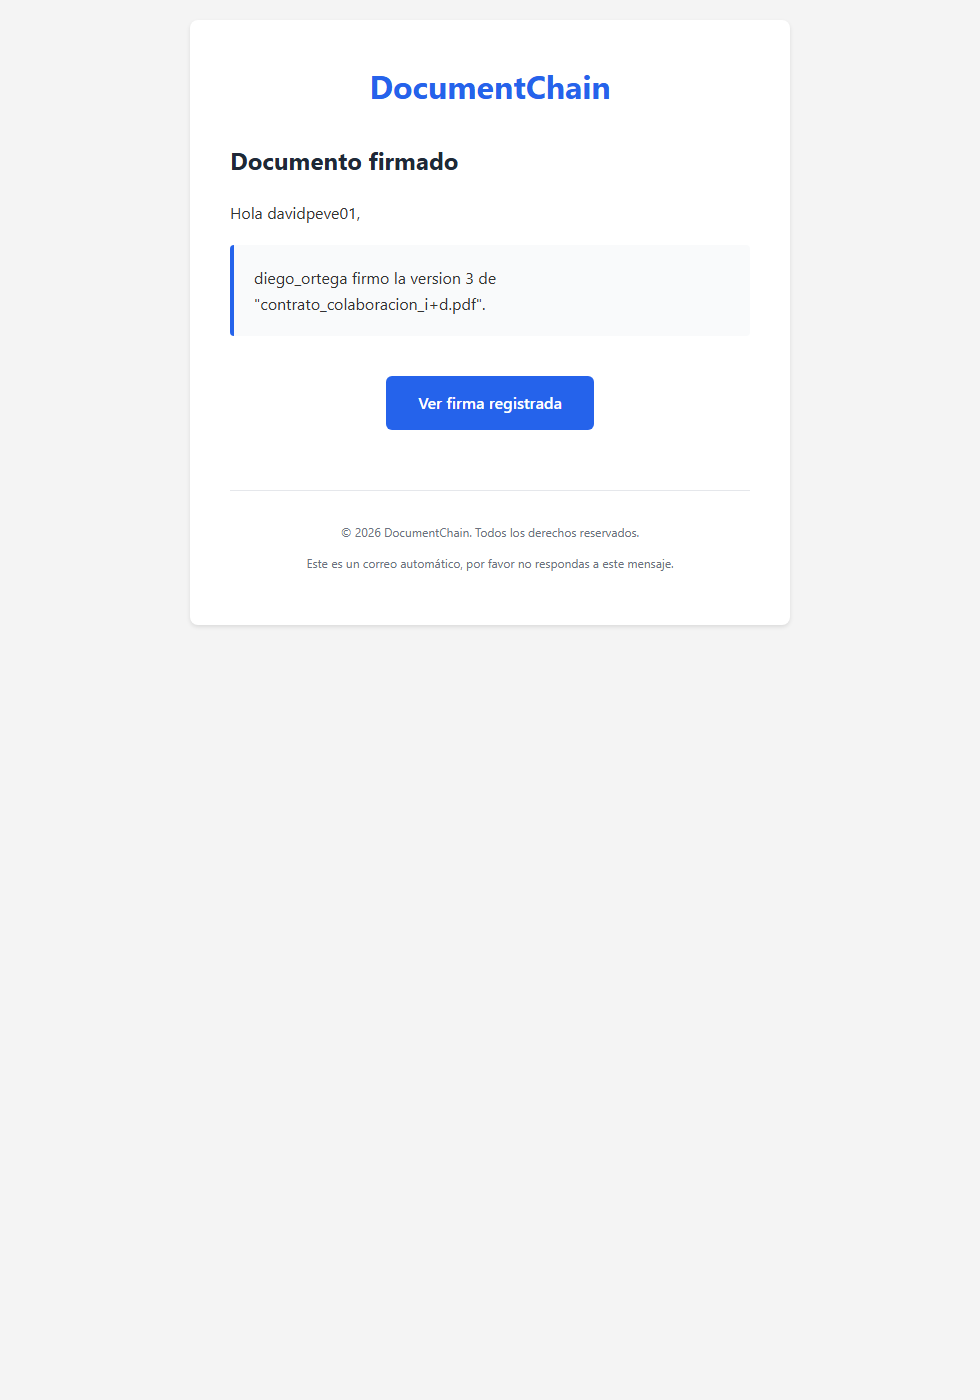
\includegraphics[width=0.78\textwidth]{capturas-ui/email-document-signed-preview.png}
    \caption{Correo transaccional de documento firmado}
    \label{fig:email-document-signed-preview}
\end{figure}

\subsubsection{Configurar preferencias de notificaciones}

\begin{enumerate}
    \item Accede a \textbf{Configuración} desde el icono de engranaje.
    \item Dentro de la pestaña \textbf{Seguridad y Cuenta}, localiza la sección Notificaciones.
    \item Activa/desactiva:
    \begin{itemize}
        \item Notificaciones in-app
        \item Notificaciones push
        \item Emails
        \item Por tipo de evento
    \end{itemize}
    \item Los cambios se guardan automáticamente.
\end{enumerate}

\subsection{Configuración de cuenta}

\begin{figure}[H]
    \centering
    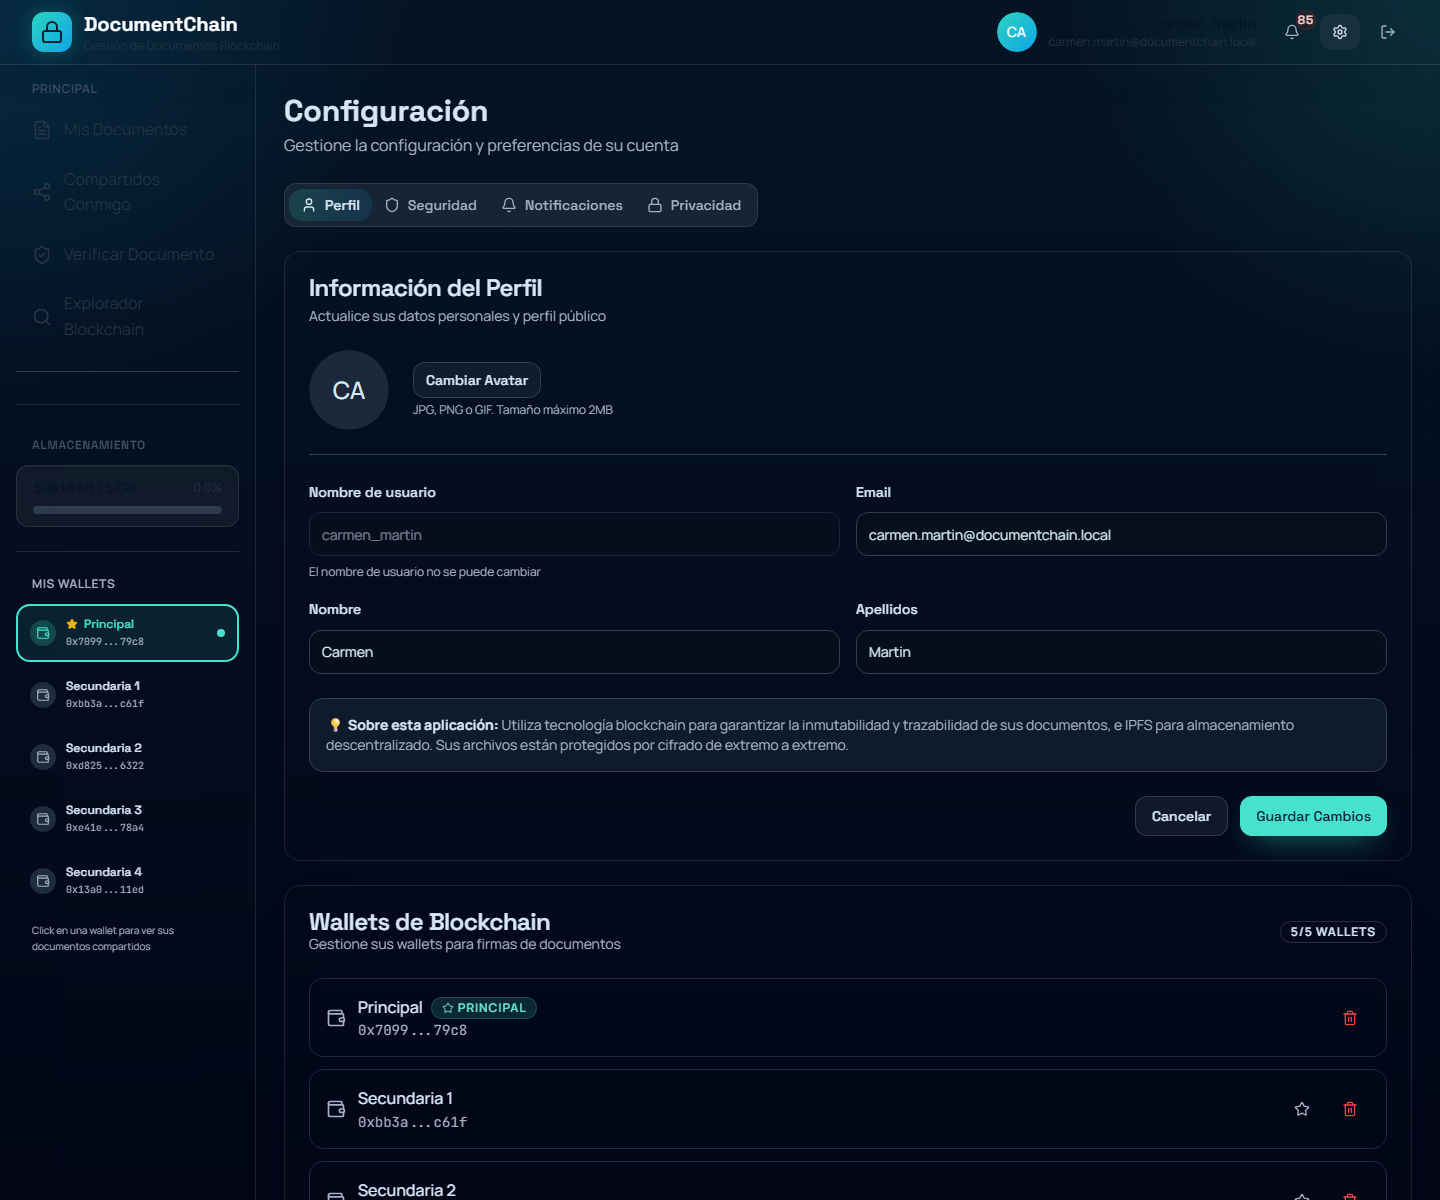
\includegraphics[width=0.95\textwidth]{capturas-ui/settings-page.png}
    \caption{Página de configuración de la cuenta (escritorio)}
    \label{fig:settings-page}
\end{figure}

\begin{figure}[H]
    \centering
    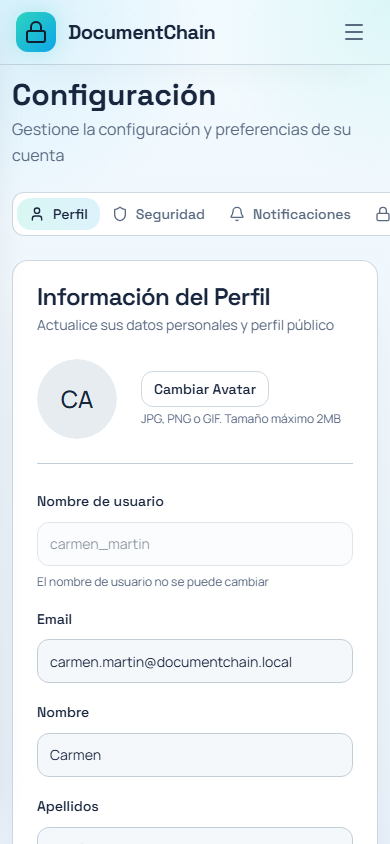
\includegraphics[width=0.45\textwidth]{capturas-ui/mobile-settings.png}
    \caption{Página de configuración de la cuenta (móvil)}
    \label{fig:settings-page-mobile}
\end{figure}

\subsubsection{Editar información personal y avatar}

\begin{enumerate}
    \item Accede a \textbf{Configuración}.
    \item En la pestaña \textbf{Perfil}, puedes:
    \begin{itemize}
        \item Subir o eliminar tu \textbf{foto de perfil} (JPG, PNG o GIF, máximo 2\,MB)
        \item Editar nombre y apellidos
        \item Editar email (requiere re-verificación)
        \item Consultar el nombre de usuario (no editable)
    \end{itemize}
    \item Haz clic en \textbf{Guardar cambios}.
\end{enumerate}

La foto de perfil se almacena localmente en el servidor y se muestra tanto en la cabecera de la aplicación como en la vista de perfil. Cualquier usuario que consulte tu perfil podrá ver la imagen.

\begin{figure}[H]
    \centering
    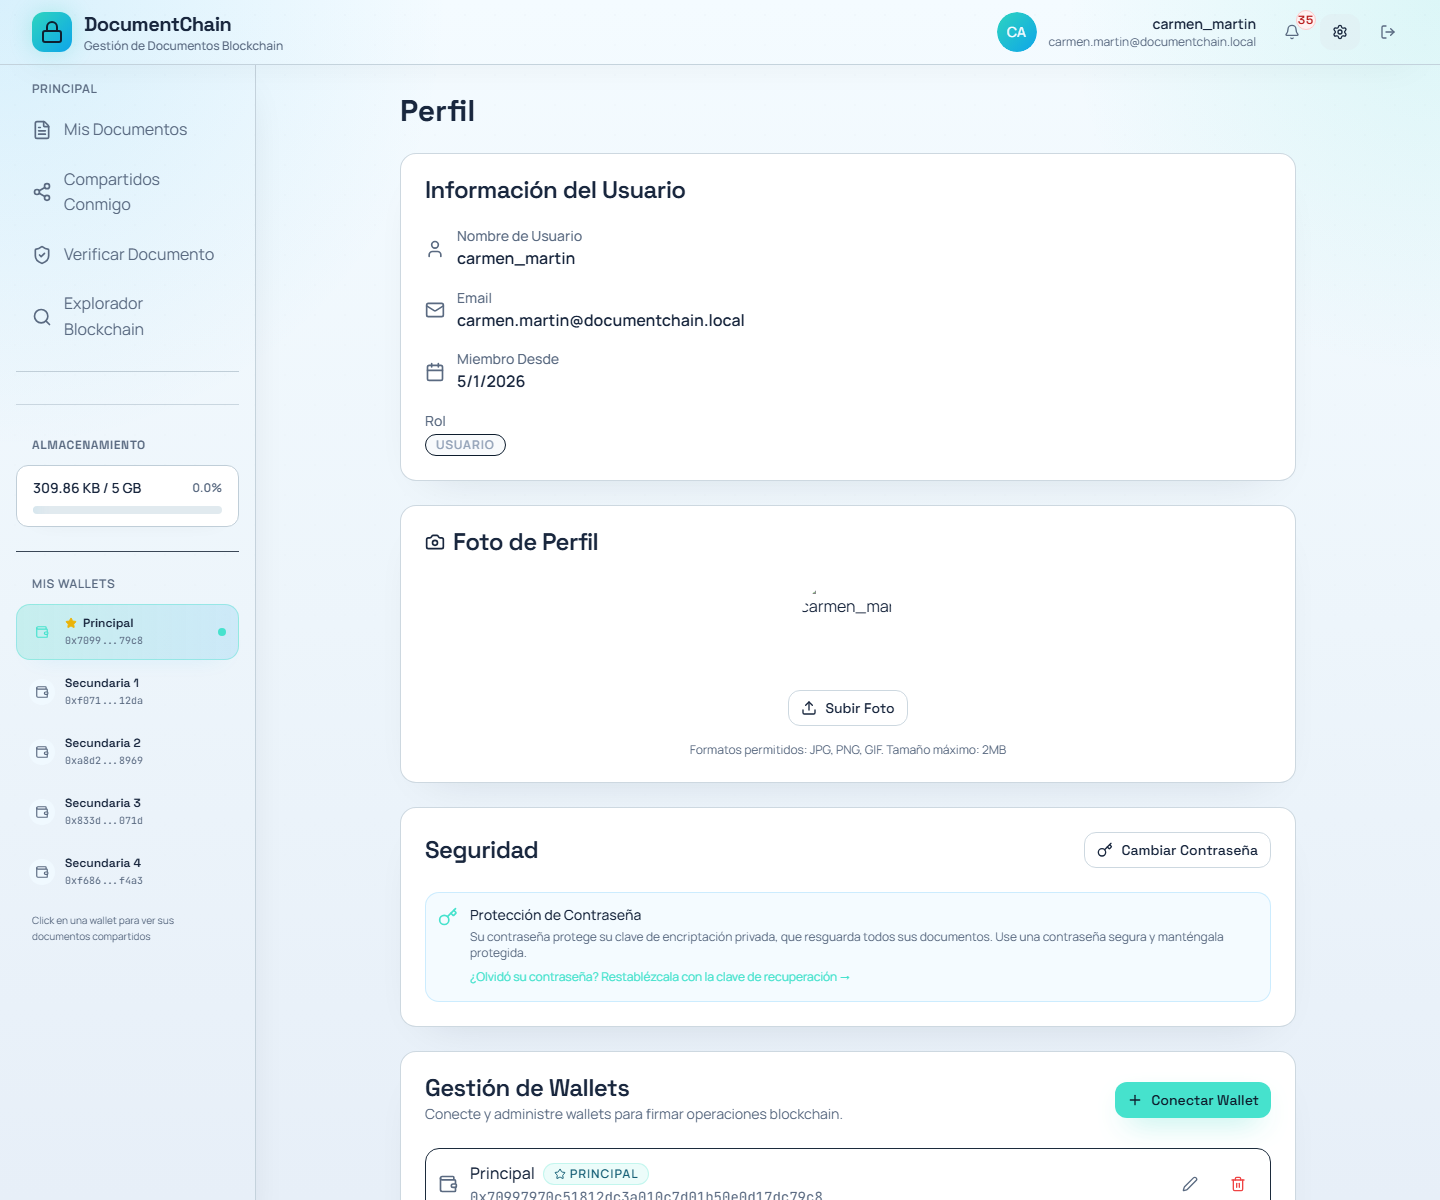
\includegraphics[width=0.95\textwidth]{capturas-ui/profile-page.png}
    \caption{Vista de perfil del usuario con gestión guiada de wallet}
    \label{fig:profile-page}
\end{figure}

La ruta \texttt{/app/profile} complementa a \texttt{/app/settings} y concentra la información identificativa, el avatar y la conexión guiada de wallets cuando el usuario viene de un flujo que requiere firma blockchain.

\subsubsection{Usar la vista de perfil y la conexión guiada de wallet}

\begin{enumerate}
    \item Accede a \texttt{/app/profile} desde un flujo que requiera conectar una wallet o desde el menú lateral de la aplicación.
    \item En esta pantalla puedes consultar tu nombre de usuario, email, fecha de alta y rol asignado.
    \item El bloque de avatar permite subir una imagen nueva o eliminar la existente.
    \item Si has llegado desde una operación que necesita firma blockchain, la página mostrará un aviso y abrirá el gestor de wallets para completar la conexión.
    \item Una vez conectada la wallet correctamente, la aplicación puede redirigirte de vuelta al flujo pendiente para continuar la operación.
\end{enumerate}

\subsubsection{Gestionar wallets}

\begin{enumerate}
    \item En \texttt{/app/settings}, dentro de la pestaña \textbf{Perfil}, revisa el bloque \textbf{Wallets de Blockchain}.
    \item Las wallets se guardan automáticamente cuando se usan por primera vez para subir, compartir, versionar, firmar o reactivar la cuenta.
    \item En la captura del anexo se muestra un caso con el límite completo de wallets registradas, de modo que puede comprobarse el contador \textbf{5/5} visible en la interfaz.
    \item Desde ese bloque puedes:
    \begin{itemize}
        \item Marcar una wallet como \textbf{principal}
        \item Eliminar una wallet ya registrada
        \item Confirmar cuántas wallets tienes guardadas de un máximo de cinco
    \end{itemize}
    \item Para establecer una como principal, haz clic en la estrella.
    \item Para eliminar, usa el icono de papelera de la fila correspondiente.
\end{enumerate}

\textbf{Nota}: Puedes tener hasta 5 wallets conectadas. La wallet principal se usa por defecto para transacciones.

\subsubsection{Cambiar contraseña}

\begin{enumerate}
    \item Ve a la pestaña \textbf{Seguridad y Cuenta}.
    \item Introduce:
    \begin{itemize}
        \item Contraseña actual
        \item Nueva contraseña
        \item Confirmar nueva contraseña
    \end{itemize}
    \item Haz clic en \textbf{Actualizar contraseña}.
\end{enumerate}

\textcolor{orange}{\textbf{Importante}}: Al cambiar la contraseña, tu clave privada se re-encriptará con la nueva contraseña. Asegúrate de recordarla.

Tras completarse el cambio, se envía un correo de confirmación con la fecha y hora del evento y un acceso directo a la configuración de seguridad. Esta notificación permite revisar con rapidez el estado de la cuenta cuando se detecta una modificación no esperada.

\begin{figure}[H]
    \centering
    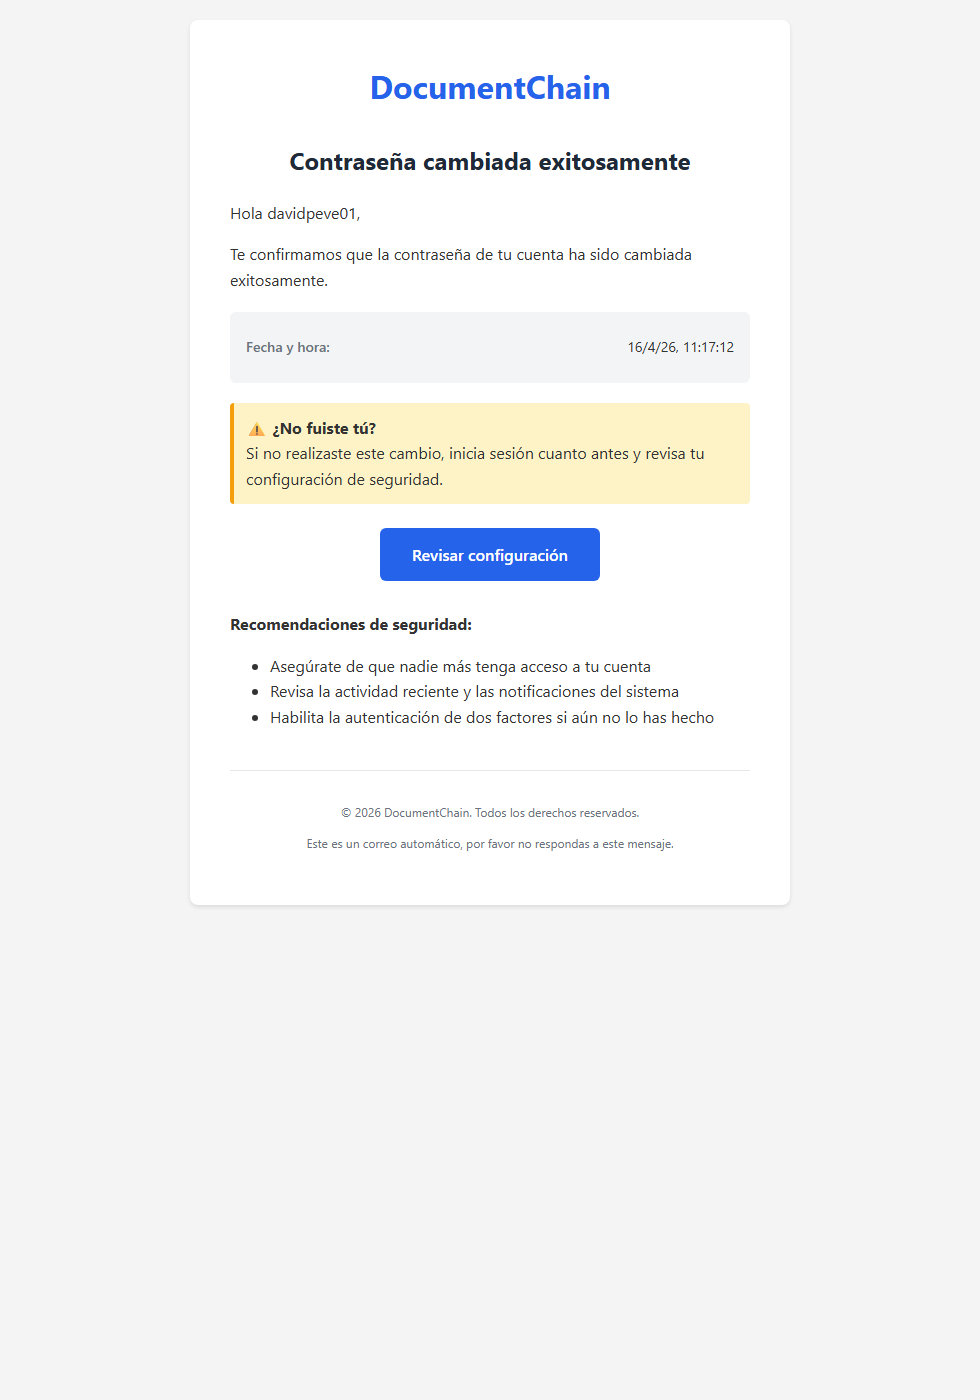
\includegraphics[width=0.78\textwidth]{capturas-ui/email-password-changed-preview.png}
    \caption{Correo de confirmación tras el cambio de contraseña}
    \label{fig:email-password-changed-preview}
\end{figure}

\subsubsection{Activar autenticación de dos factores (2FA)}

\begin{enumerate}
    \item En la pestaña \textbf{Seguridad y Cuenta}, pulsa \textbf{Configurar 2FA}.
    \item Se mostrará un código QR y un secreto alternativo para configuración manual.
    \item Abre tu app de autenticación (Google Authenticator, Authy, etc.).
    \item Escanea el código QR.
    \item Introduce el código de 6 dígitos generado por la app.
    \item Tras la verificación, el sistema generará códigos de respaldo de un solo uso. \textbf{Guárdalos en lugar seguro}.
    \item Más adelante podrás regenerar esos códigos o desactivar el 2FA introduciendo un código TOTP válido.
\end{enumerate}

\begin{figure}[H]
    \centering
    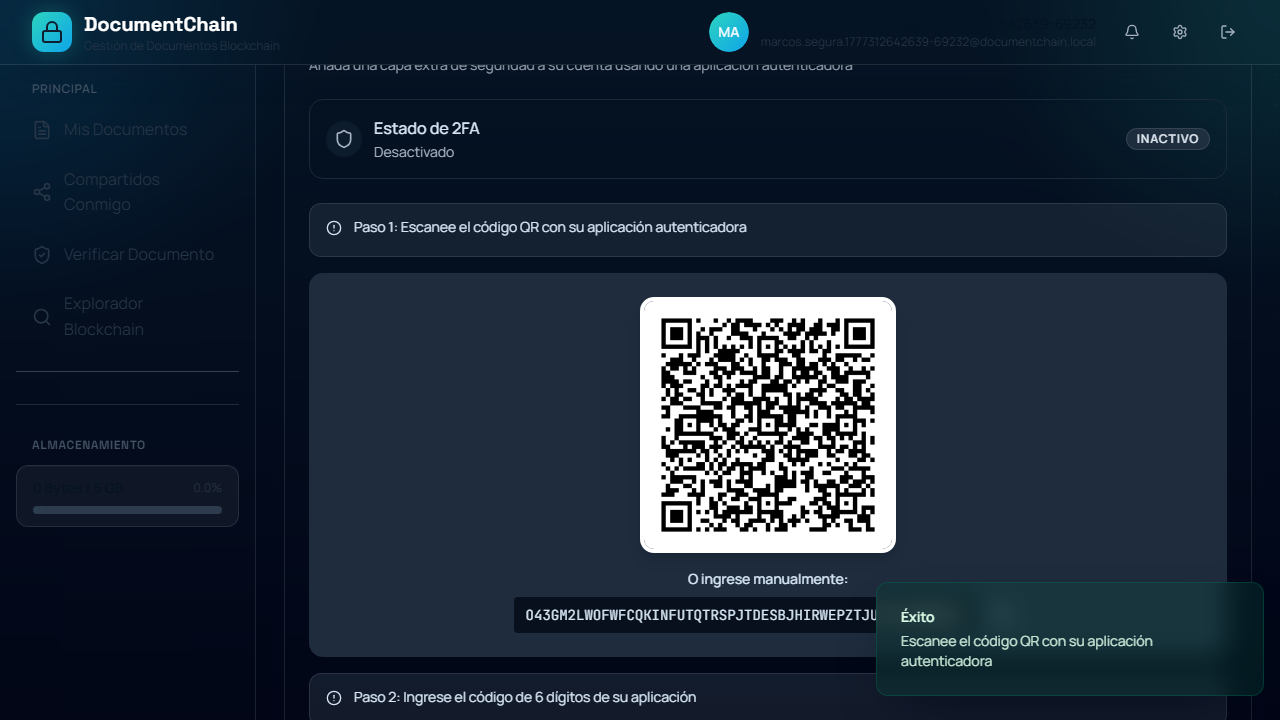
\includegraphics[width=0.95\textwidth]{capturas-ui/two-factor-setup.png}
    \caption{Configuración de segundo factor (2FA) (escritorio)}
    \label{fig:two-factor-setup}
\end{figure}

\begin{figure}[H]
    \centering
    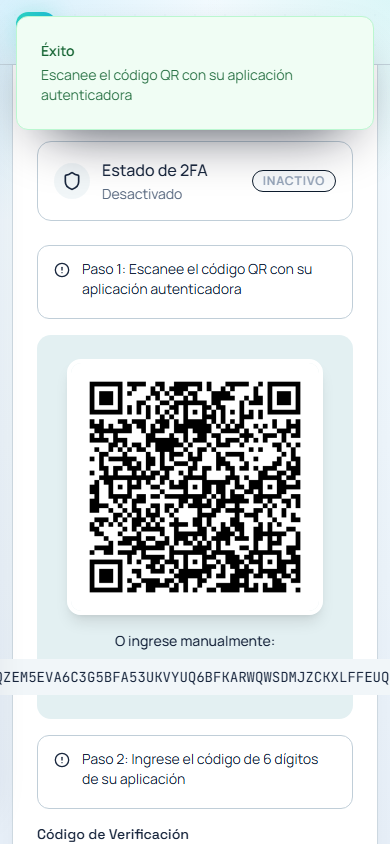
\includegraphics[width=0.45\textwidth]{capturas-ui/mobile-2fa-setup.png}
    \caption{Configuración de segundo factor (2FA) (móvil)}
    \label{fig:two-factor-setup-mobile}
\end{figure}

Desde ahora, al iniciar sesión se te pedirá código 2FA tras la contraseña.

\subsubsection{Regenerar códigos de respaldo o desactivar 2FA}

\begin{enumerate}
    \item Vuelve al bloque de \textbf{2FA} dentro de la pestaña \textbf{Seguridad y Cuenta}.
    \item Para regenerar códigos de respaldo, pulsa la opción correspondiente e introduce un código temporal válido de tu aplicación autenticadora.
    \item El sistema invalidará los códigos anteriores y mostrará un nuevo conjunto una única vez para que puedas guardarlo.
    \item Si necesitas desactivar el 2FA, usa la acción \textbf{Desactivar 2FA} y confirma también con un código temporal válido.
\end{enumerate}

\subsubsection{Seguridad, notificaciones y zona de peligro}

La pestaña \textbf{Seguridad y Cuenta} agrupa todas las opciones relacionadas con la protección y gestión de la cuenta:

\begin{enumerate}
    \item \textbf{Contraseña}: cambia la contraseña actual. Tras el cambio se envía un email de confirmación y se cierra la sesión.
    \item \textbf{Autenticación de dos factores (2FA)}: configura, regenera códigos de respaldo o desactiva el 2FA.
    \item \textbf{Notificaciones}: activa o desactiva avisos por email (documentos compartidos, nuevas versiones) y notificaciones push en la aplicación.
    \item \textbf{Zona de Peligro}:
    \begin{itemize}
        \item \textbf{Suspender cuenta}: bloquea temporalmente tu wallet en blockchain. Requiere firma con la wallet principal. Puedes reactivarla cuando quieras.
        \item \textbf{Eliminar cuenta}: elimina permanentemente tu usuario y todos tus datos de la base de datos. Desancla los archivos de IPFS y deja inmutables los registros en blockchain. Requiere firmar \texttt{suspendMyself} con la wallet principal.
    \end{itemize}
\end{enumerate}

\subsubsection{Reactivar una cuenta suspendida}

\begin{enumerate}
    \item Si la cuenta está suspendida, el sistema te mantendrá en \texttt{/app/settings} y dejará accesible la pestaña \textbf{Seguridad y Cuenta}.
    \item Pulsa \textbf{Reactivar cuenta}.
    \item Selecciona y conecta la \textbf{wallet principal} asociada a la cuenta.
    \item Firma la transacción de reactivación y espera la confirmación on-chain.
    \item Cuando el backend valide la operación, se restaurará el acceso normal al resto de vistas autenticadas.
\end{enumerate}

\section{Manual de Administrador}

\subsection{Acceso al panel de administración}

Solo usuarios con rol \textbf{ADMIN} pueden acceder.

\begin{enumerate}
    \item Inicia sesión con tu cuenta de administrador.
    \item En la barra lateral aparecerá la entrada \textbf{Panel}.
    \item Haz clic para acceder a \texttt{/app/dashboard}.
\end{enumerate}

\begin{figure}[H]
    \centering
    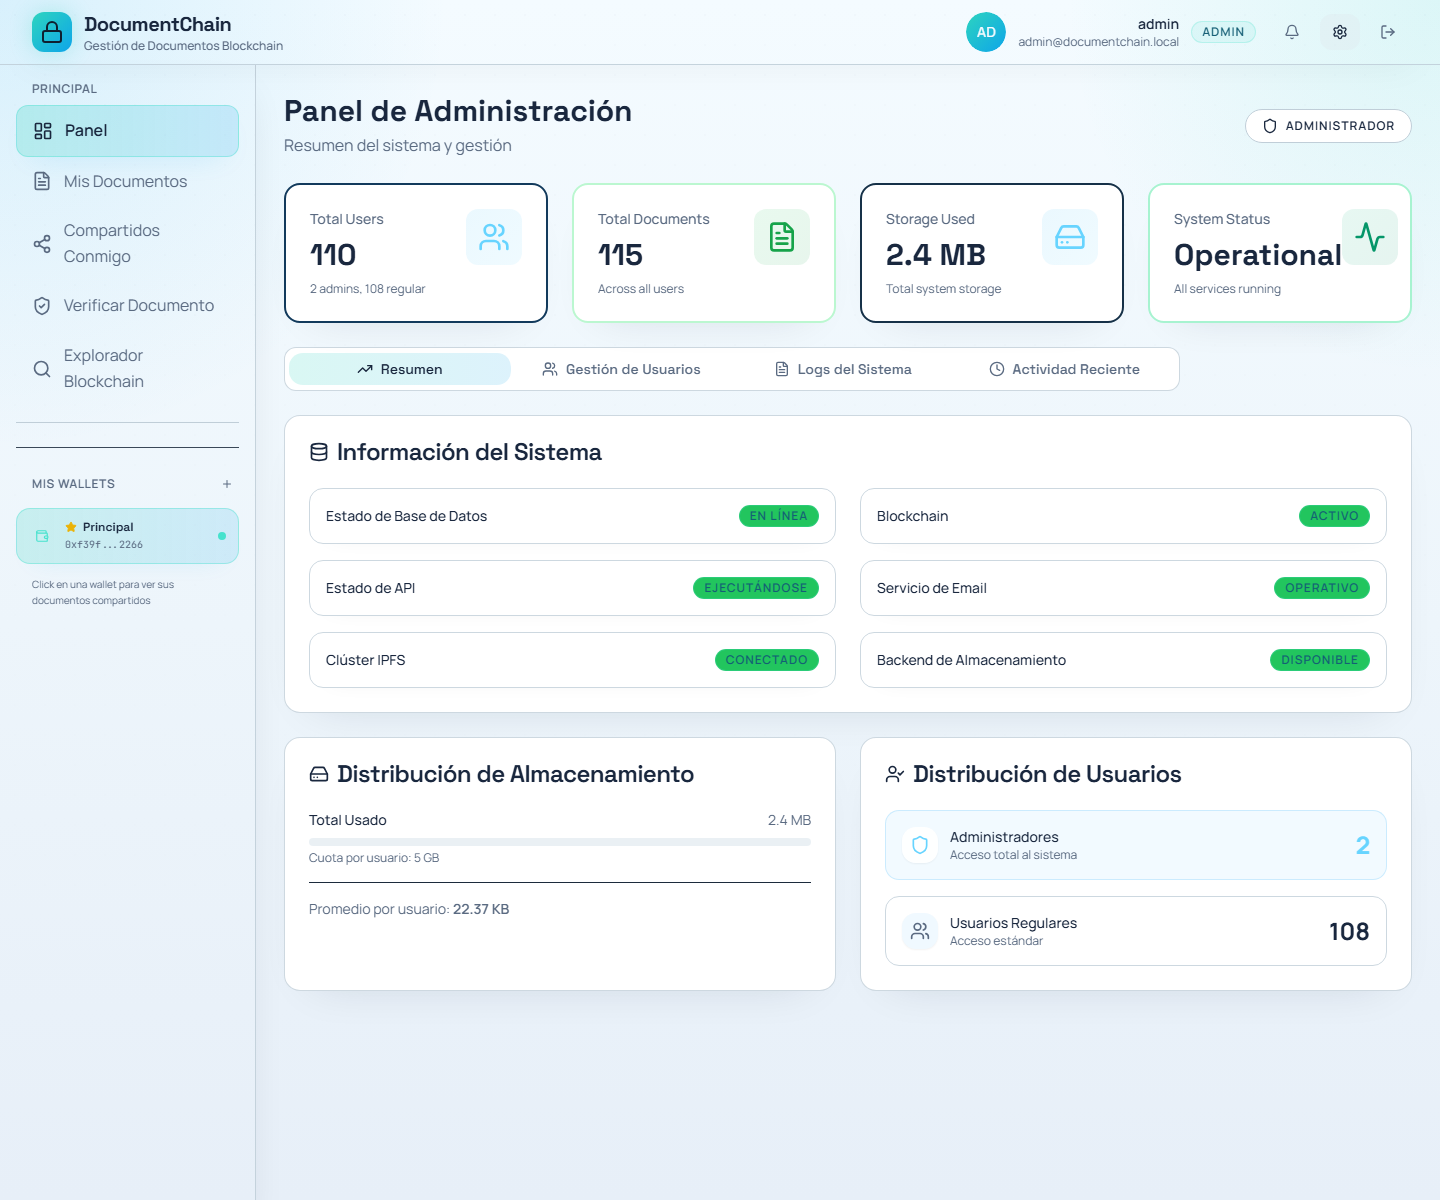
\includegraphics[width=0.95\textwidth]{capturas-ui/admin-dashboard.png}
    \caption{Panel de administración con estadísticas globales (escritorio)}
    \label{fig:admin-dashboard}
\end{figure}

\begin{figure}[H]
    \centering
    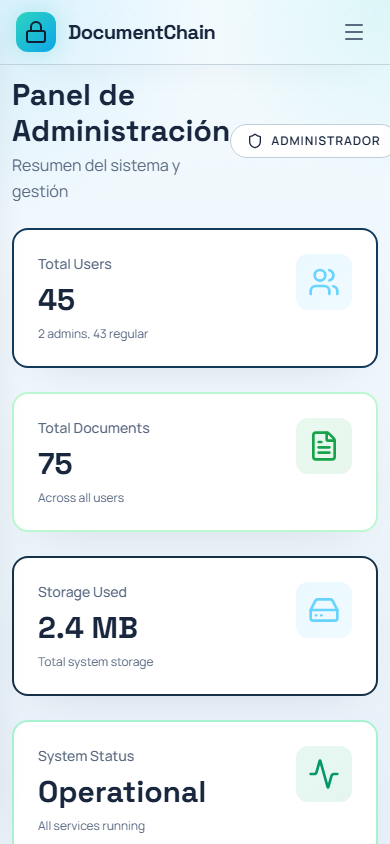
\includegraphics[width=0.45\textwidth]{capturas-ui/mobile-admin-dashboard.png}
    \caption{Panel de administración con estadísticas globales (móvil)}
    \label{fig:admin-dashboard-mobile}
\end{figure}

\subsection{Gestión de usuarios}

\subsubsection{Ver lista de usuarios}

\begin{enumerate}
    \item En el panel de administración, entra en la pestaña \textbf{Gestión de Usuarios}.
    \item Verás dos bloques principales: \textbf{Administradores} y \textbf{Usuarios Regulares}.
    \item Información visible:
    \begin{itemize}
        \item Username y email
        \item Rol (USER o ADMIN)
        \item Fecha de registro
        \item Total de wallets registradas
        \item Total de documentos
        \item Contador de sesiones y estado del 2FA al desplegar el detalle
    \end{itemize}
\end{enumerate}

\begin{figure}[H]
    \centering
    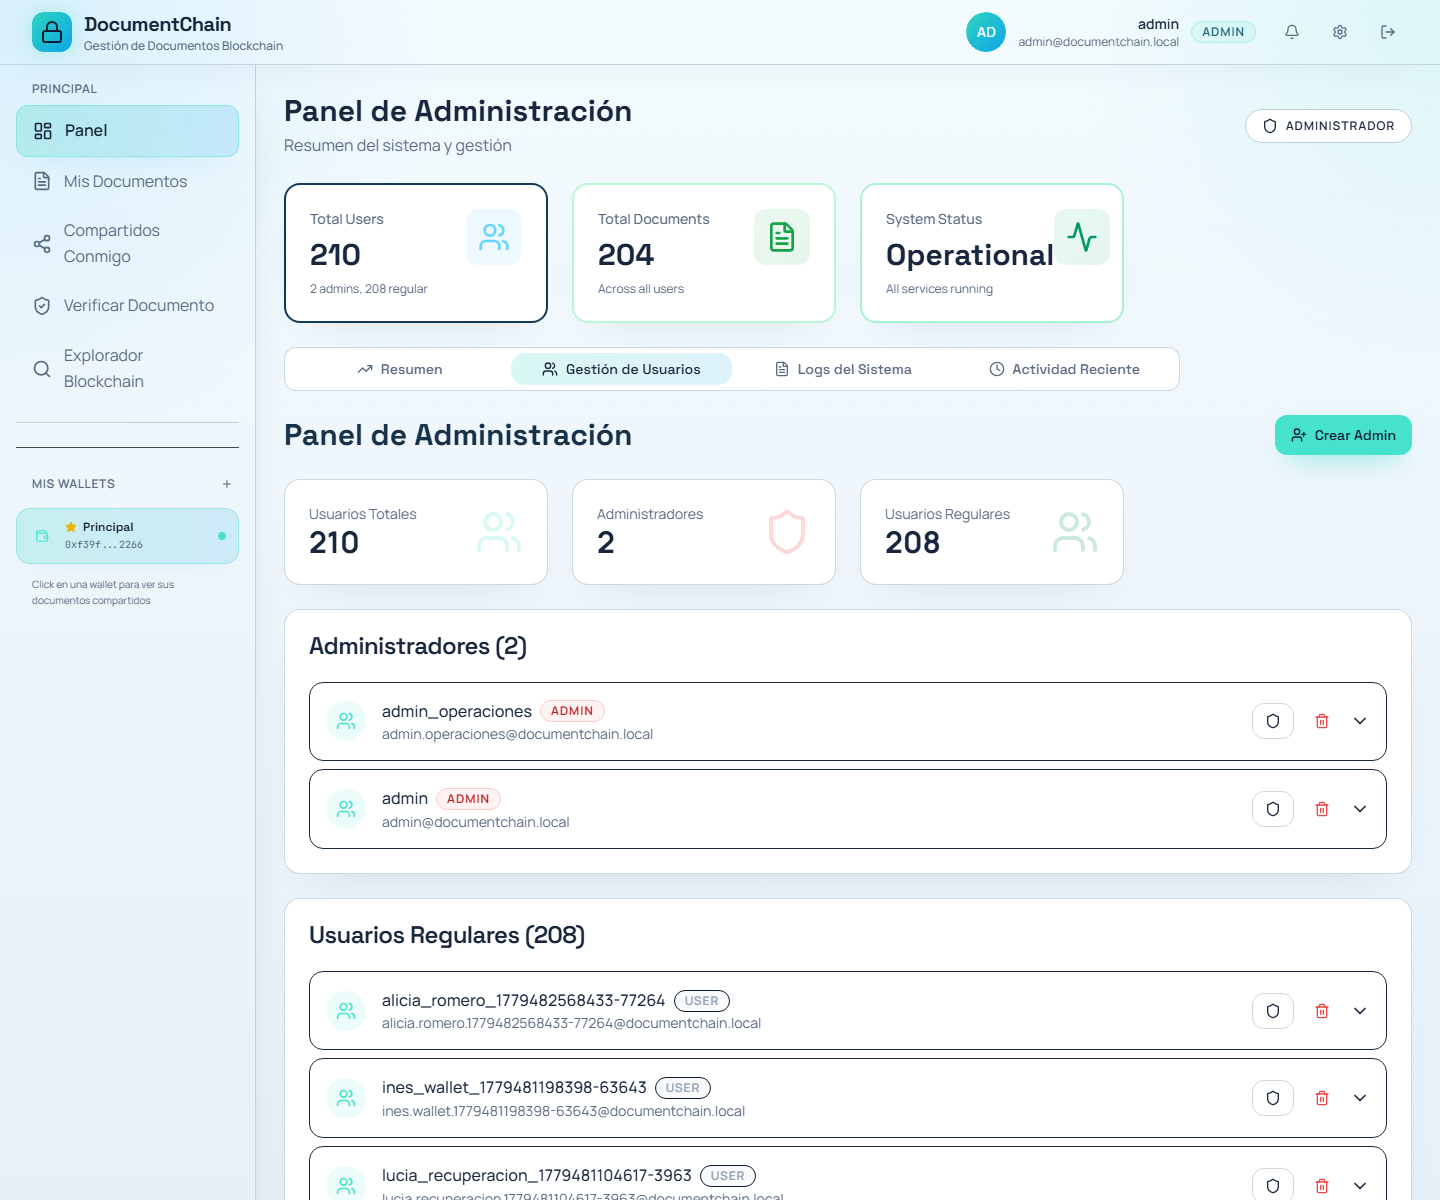
\includegraphics[width=0.95\textwidth]{capturas-ui/admin-users-tab.png}
    \caption{Gestión de usuarios en el panel de administración}
    \label{fig:admin-users-tab}
\end{figure}

\subsubsection{Crear un nuevo administrador}

\begin{enumerate}
    \item En la pestaña \textbf{Gestión de Usuarios}, pulsa \textbf{Crear Admin}.
    \item Completa username, email, contraseña y nombre completo.
    \item Confirma el alta.
    \item El sistema devolverá una \textbf{Recovery Key} que debe guardarse inmediatamente.
\end{enumerate}

\subsubsection{Inspeccionar el detalle de un usuario}

\begin{enumerate}
    \item Haz clic sobre una fila para expandirla.
    \item El panel ampliado muestra nombre completo, fecha de creación, número de documentos, wallets registradas, contador de sesiones y estado de 2FA.
\end{enumerate}

\subsubsection{Cambiar rol de un usuario}

\begin{enumerate}
    \item En la fila del usuario, pulsa el botón de escudo.
    \item El sistema promocionará a ADMIN o degradará a USER según el rol actual.
    \item Confirma la acción.
\end{enumerate}

\textbf{Advertencia}: Otorgar rol ADMIN da acceso completo al panel de administración.

\subsubsection{Eliminar una cuenta}

\textcolor{orange}{\textbf{Advertencia crítica}}: Eliminar una cuenta es irreversible.

\begin{enumerate}
    \item En la fila del usuario, pulsa el icono de papelera.
    \item Confirma la operación desde el diálogo del navegador.
    \item La cuenta dejará de estar disponible en la aplicación.
    \item Las evidencias ya registradas en blockchain seguirán existiendo porque forman parte del historial inmutable del sistema.
\end{enumerate}

\subsection{Estadísticas del sistema}

\begin{enumerate}
    \item En \texttt{/app/dashboard}, revisa la pestaña \textbf{Resumen}.
    
    \begin{figure}[H]
        \centering
        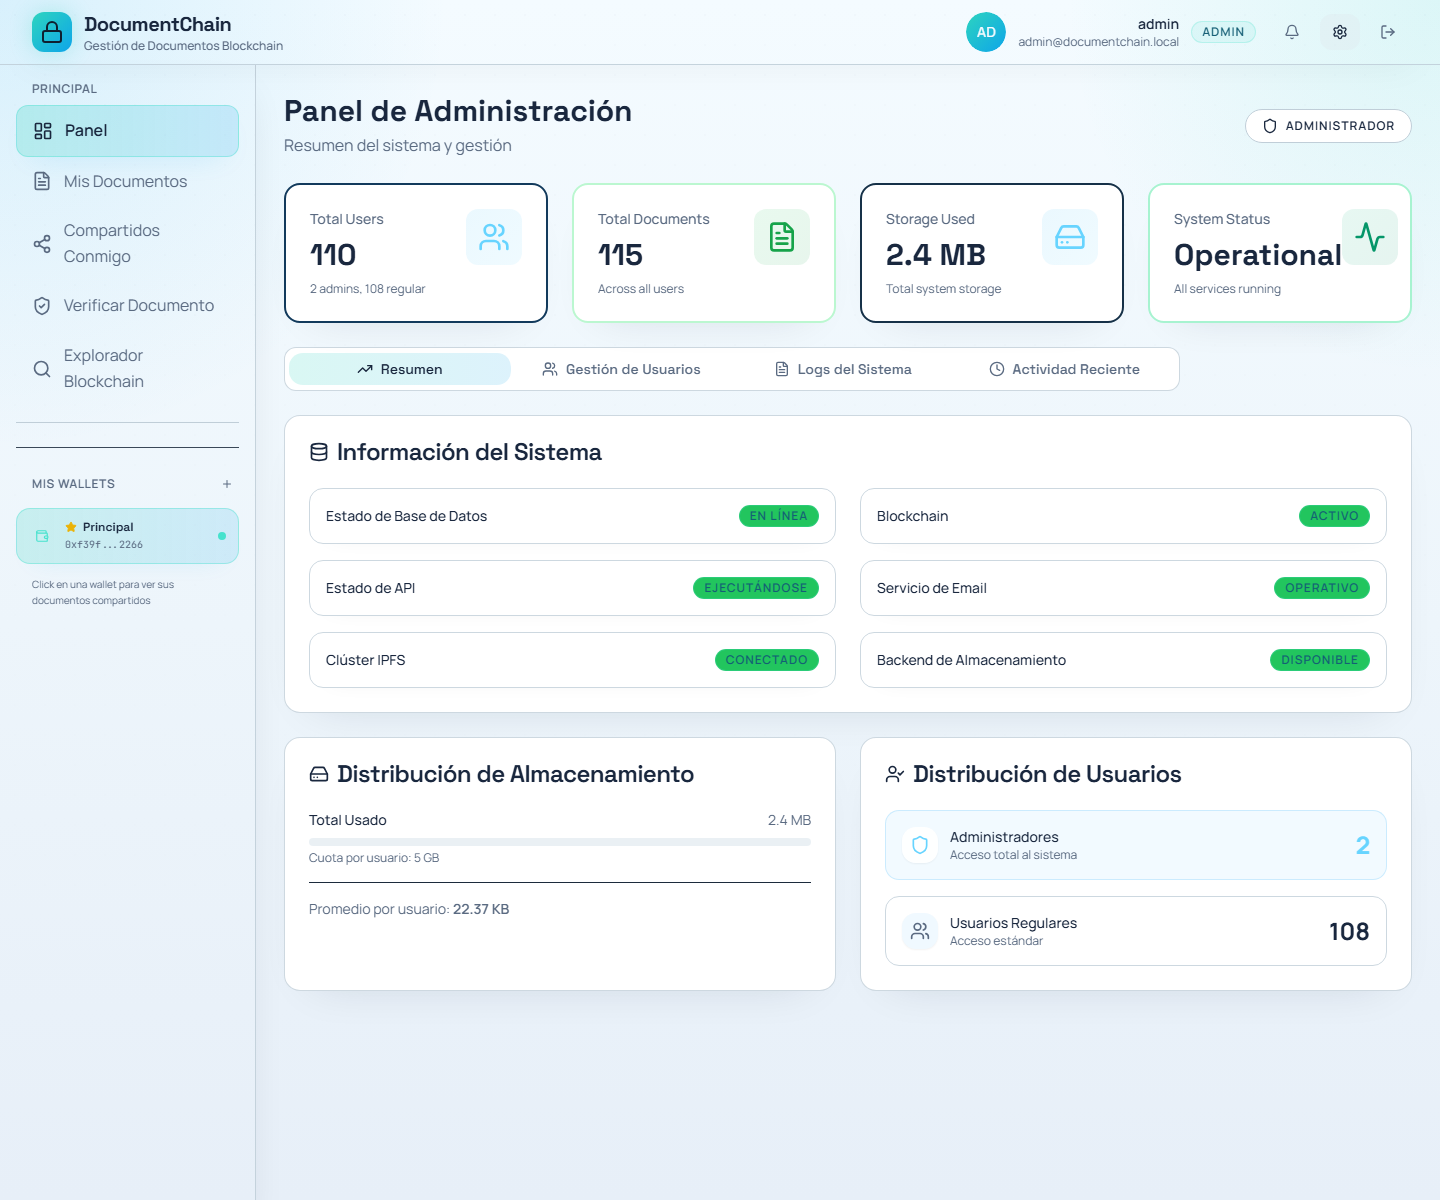
\includegraphics[width=0.95\textwidth]{capturas-ui/admin-dashboard.png}
        \caption{Resumen y métricas globales del sistema}
        \label{fig:system-stats}
    \end{figure}
    
    \item Métricas disponibles:
    \begin{itemize}
        \item Tarjetas resumen con \textbf{usuarios totales}, \textbf{documentos totales}, \textbf{almacenamiento usado} y \textbf{estado general del sistema}
        \item Estado operativo de \textbf{base de datos}, \textbf{API}, \textbf{nodo IPFS}, \textbf{blockchain}, \textbf{servicio de email} y \textbf{backend de almacenamiento}
        \item Distribución de almacenamiento y promedio por usuario
        \item Distribución entre \textbf{administradores} y \textbf{usuarios regulares}
    \end{itemize}
\end{enumerate}

\subsubsection{Revisar la actividad reciente}

\begin{enumerate}
    \item Dentro de \texttt{/app/dashboard}, abre la pestaña \textbf{Actividad Reciente}.
    \item La vista muestra los usuarios registrados más recientemente.
    \item Para cada entrada se presenta nombre de usuario, email, rol y fecha de alta.
    \item Esta pestaña resulta útil para detectar registros inesperados, comprobar altas recientes o revisar si una promoción a administrador se ha aplicado correctamente.
\end{enumerate}

\subsection{Auditoría blockchain}

\begin{enumerate}
    \item Accede a \texttt{/app/blockchain} desde la barra lateral, o usa la página pública \texttt{/audit} sin necesidad de autenticación.
    
    \begin{figure}[H]
        \centering
        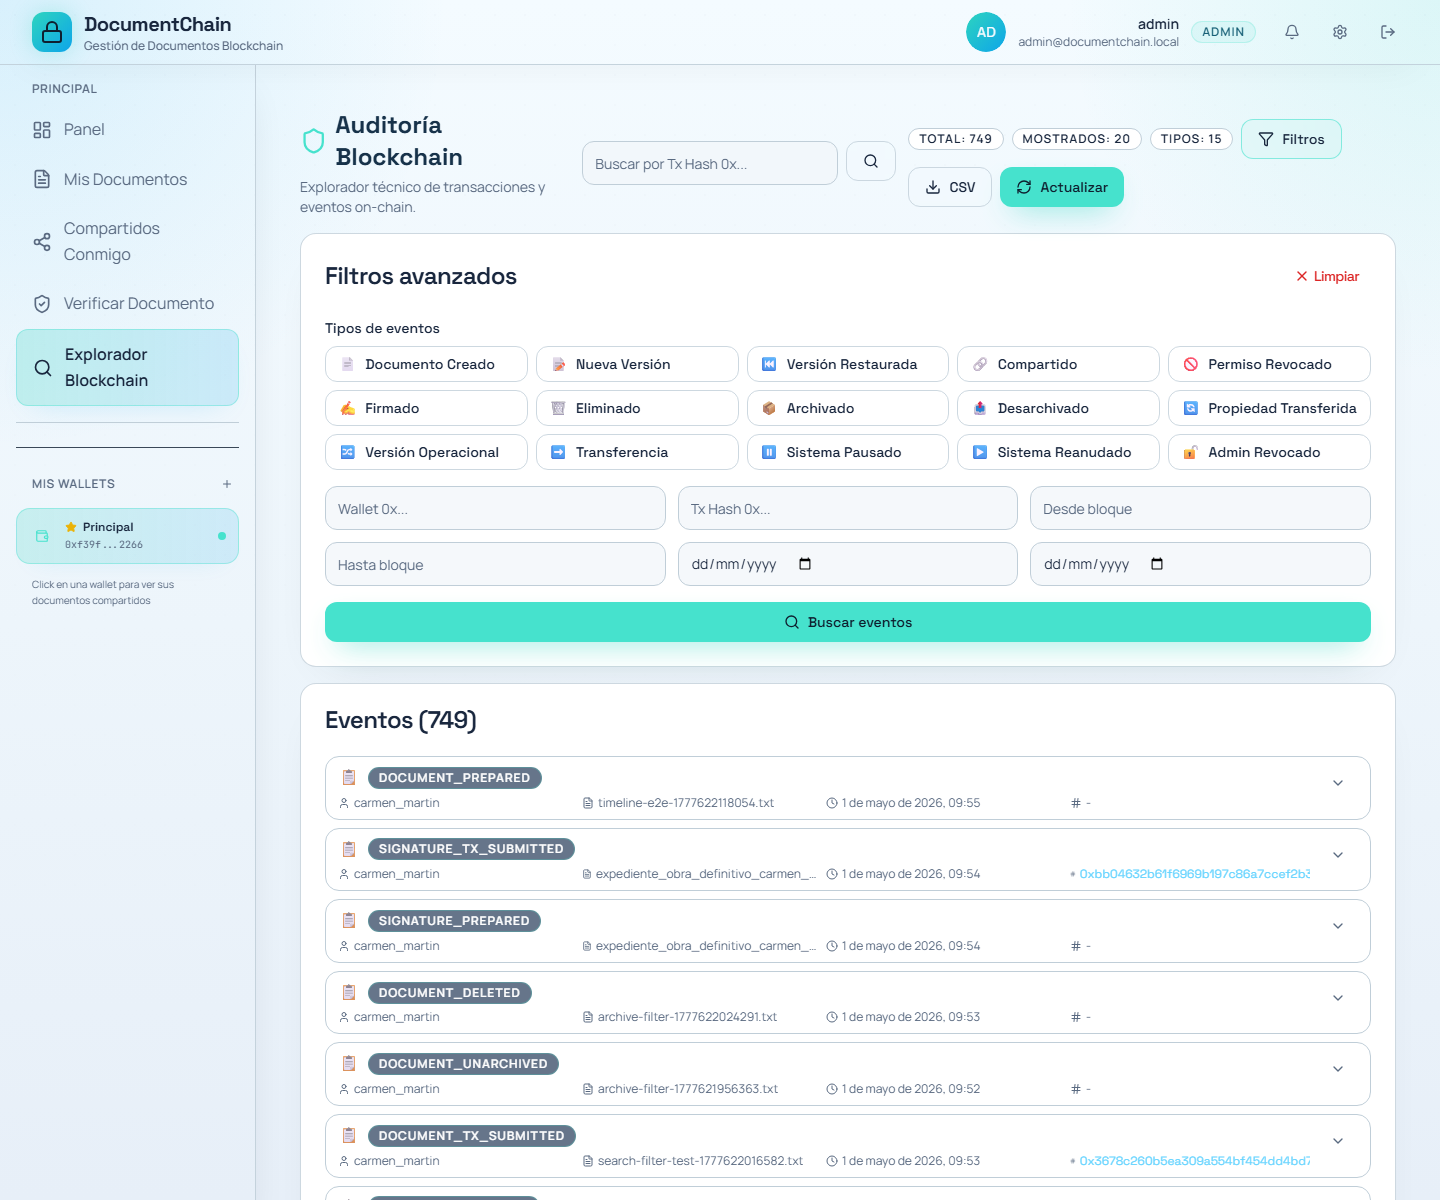
\includegraphics[width=0.95\textwidth]{capturas-ui/blockchain-auditor.png}
        \caption{Explorador blockchain con filtros y eventos (escritorio)}
        \label{fig:blockchain-auditor}
    \end{figure}
    
    \begin{figure}[H]
        \centering
        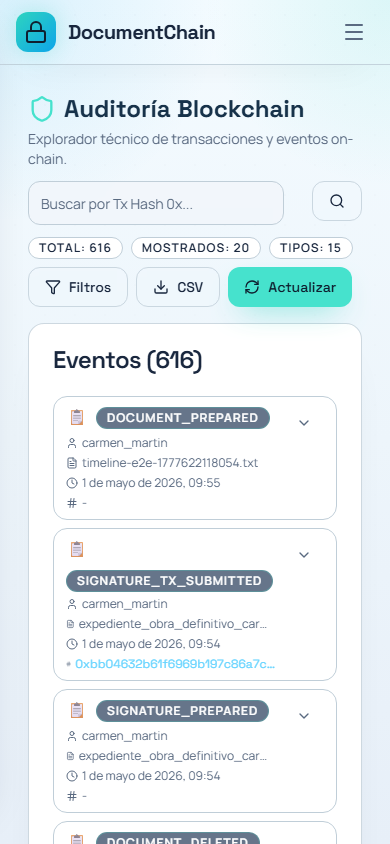
\includegraphics[width=0.45\textwidth]{capturas-ui/mobile-blockchain-auditor.png}
        \caption{Explorador blockchain con filtros y eventos (móvil)}
        \label{fig:blockchain-auditor-mobile}
    \end{figure}
    
    \item Verás:
    \begin{itemize}
        \item Tarjetas de resumen con el total disponible, los eventos mostrados y el número de tipos de evento filtrados
        \item Un panel de \textbf{filtros avanzados} por tipo de evento, wallet, hash de transacción, rango de bloques y rango temporal
        \item Un listado de \textbf{eventos recientes} en formato tabla compacta con tipo, documento, actor, bloque, fecha y hash de transacción
        \item Al hacer clic en cualquier \textbf{hash de transacción}, se abre un modal con el detalle completo de la transacción decodificada: estado, gas usado, bloque, fecha, y todos los eventos del contrato \texttt{DocumentRegistry} con sus argumentos
        \item Desde cada evento se puede navegar al documento asociado: si es público se abre la vista pública; si tienes permisos, accedes al detalle autenticado
        \item Exportación directa a \textbf{CSV}
    \end{itemize}
    
    \item \textbf{Búsqueda por hash de transacción} (también disponible en \texttt{/audit}):
    \begin{itemize}
        \item Introduce un hash de transacción válido (\texttt{0x...})
        \item El sistema consulta directamente la blockchain, recupera el \textit{receipt} y decodifica los logs usando el ABI del contrato
        \item Muestra los argumentos de cada evento de forma legible (\textit{docId}, \textit{owner}, \textit{versionNumber}, etc.)
        \item Enriquece los eventos con metadata de la base de datos: nombre del documento, \textit{publicId} y visibilidad
    \end{itemize}
\end{enumerate}

\subsubsection{Ver logs del sistema}

\begin{enumerate}
    \item En el panel de administración, abre la pestaña \textbf{Logs del Sistema}.
    \item El visor permite alternar entre logs \textbf{combined}, \textbf{error} y \textbf{blockchain}.
    \item Puedes ajustar el número de líneas mostradas y activar la recarga automática.
    \item Cada entrada indica:
    \begin{itemize}
        \item Timestamp
        \item Nivel
        \item Mensaje
        \item Detalle JSON expandible cuando existe metadata adicional
    \end{itemize}
\end{enumerate}

\begin{figure}[H]
    \centering
    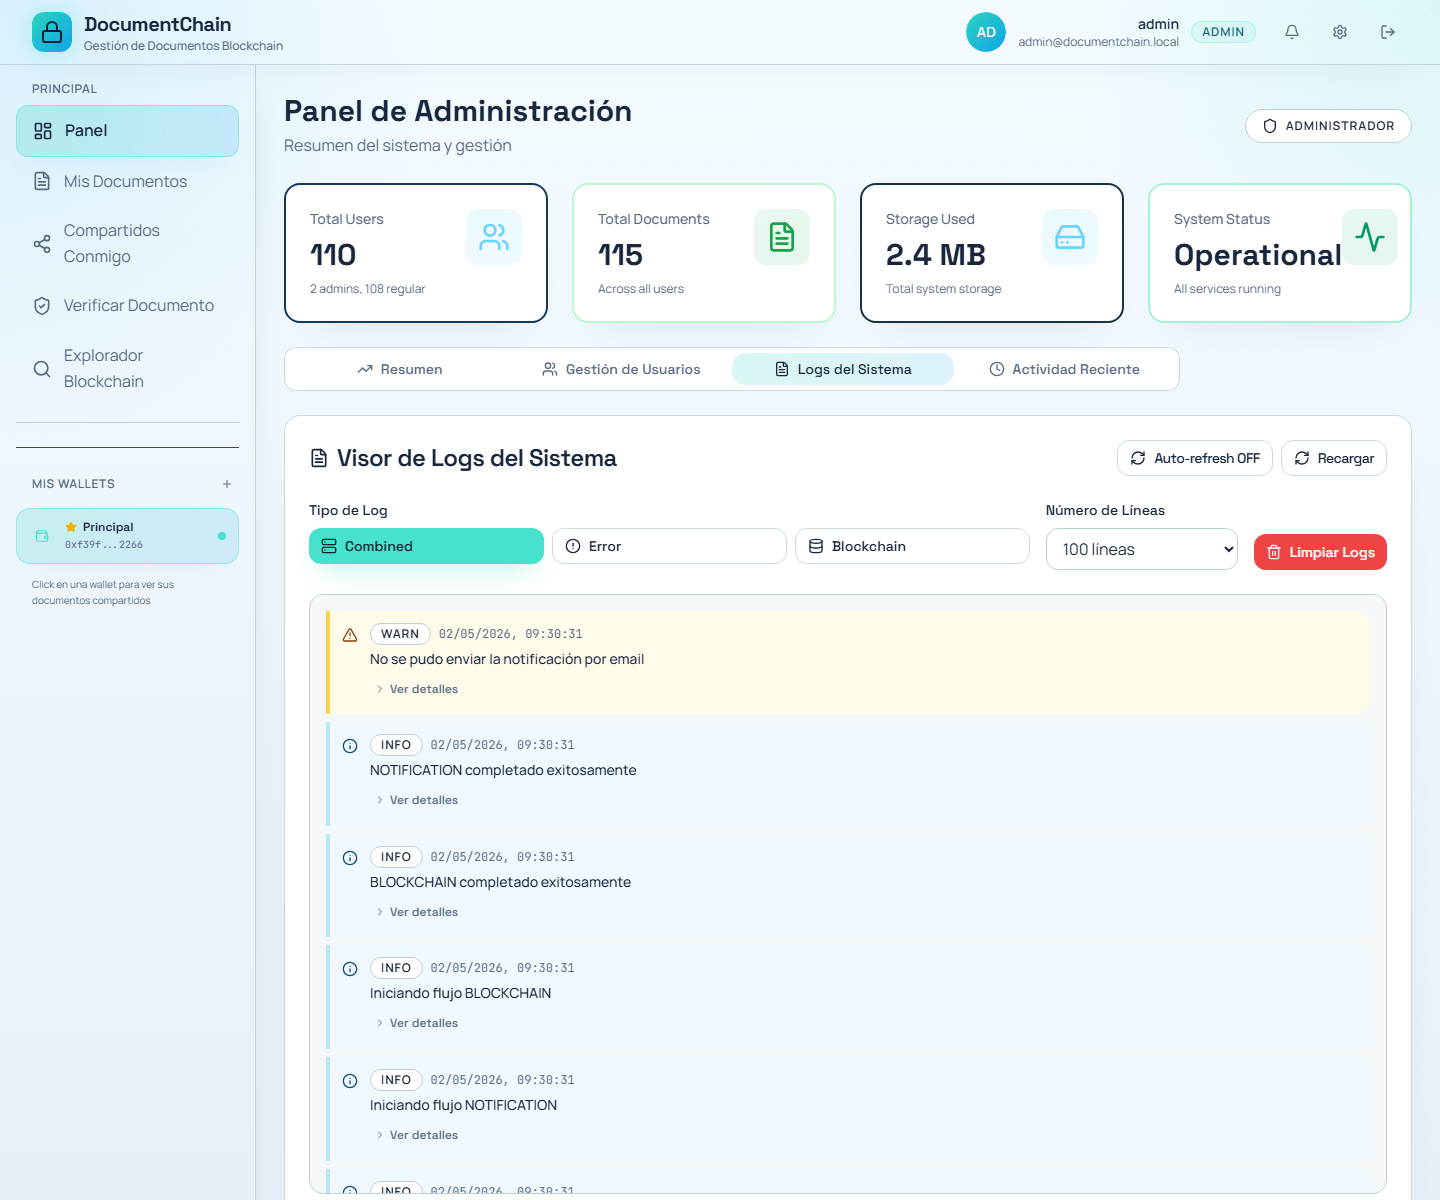
\includegraphics[width=0.95\textwidth]{capturas-ui/admin-logs-tab.png}
    \caption{Visor de logs del sistema dentro del panel de administración}
    \label{fig:admin-logs-tab}
\end{figure}



\section{Glosario}

\begin{description}
    \item[2FA] Autenticaci\'on de dos factores; en el proyecto se implementa mediante TOTP.
    \item[Blockchain] Registro distribuido e inmutable que conserva la evidencia de firmas, versiones y permisos.
    \item[BlockchainId] Identificador num\'erico asignado por el contrato \texttt{DocumentRegistry} al documento.
    \item[CID] Content Identifier, identificador \'unico de contenido en IPFS basado en hash criptogr\'afico.
    \item[CopyableId] Componente de interfaz que trunca un identificador largo y permite copiarlo al portapapeles.
    \item[DocumentId] Identificador interno del documento en la base de datos PostgreSQL.
    \item[Etiqueta] Palabra clave asociada a un documento para facilitar su clasificaci\'on y b\'usqueda.
    \item[PublicId] Identificador p\'ublico corto que permite resolver un documento publicado mediante enlace o c\'odigo QR.
    \item[TOTP] Time-based One-Time Password, c\'odigo temporal de un solo uso para autenticaci\'on de dos factores.
    \item[TxHash] Transaction Hash, identificador \'unico de una transacci\'on en la blockchain.
    \item[Wallet] Monedero de criptomonedas que permite firmar transacciones en blockchain.
\end{description}

\section*{Bibliografía}
\addcontentsline{toc}{section}{Bibliografía}

\begin{enumerate}
    \item Ethereum Foundation. (2025). \textit{Ethereum Developer Documentation}. \url{https://ethereum.org/en/developers/docs/}

    \item IPFS Project. (2025). \textit{IPFS Documentation: How IPFS Works}. \url{https://docs.ipfs.tech}

    \item Mozilla Developer Network. (2025). \textit{Web Crypto API}. \url{https://developer.mozilla.org/en-US/docs/Web/API/Web_Crypto_API}

    \item Bitwarden. (2023). \textit{End-to-End Encryption Explained}. \href{https://bitwarden.com/resources/end-to-end-encryption/}{bitwarden.com/resources/end-to-end-encryption}
\end{enumerate}

\end{document}





